\begin{appendices}

  \chapter{Tabel Himpunan $setBit$ Setelah Fungsi Preprocess Dijalankan}
  \setcounter{table}{0}
  \renewcommand{\thetable}{A.\arabic{table}}
  \renewcommand{\thefigure}{A.\arabic{figure}}
  
  \begin{table}[H]
  	\centering
  	\begin{tabular} {|l|l|l|l|l|l|l|l|l|l|l|} \hline
  		\backslashbox{$Num$}{$index$} & $ 0 $ & $ 1 $ & $ 2 $ & $ 3 $ & $ 4 $ & $ 5 $ & $ 6 $ & $ 7 $ & $ 8 $ & $ 9 $ \\ \hline
  		$ 0 $ &  - &  - &  - &  - &  - &  - &  - &  - &  - &  -   \\ \hline
  		$ 1 $ & $ 0 $ & - &  - &  - &  - &  - &  - &  - &  - &  -   \\ \hline
  		$ 2 $ & $ 1 $ & - &  - &  - &  - &  - &  - &  - &  - &  -   \\ \hline
  		$ 3 $ & $ 0 $ &$ 1 $ & - &  - &  - &  - &  - &  - &  - &  -   \\ \hline
  		$ 4 $ & $ 2 $ & - &  - &  - &  - &  - &  - &  - &  - &  -   \\ \hline
  		$ 5 $ & $ 0 $ &$ 2 $ & - &  - &  - &  - &  - &  - &  - &  -   \\ \hline
  		$ 6 $ & $ 1 $ &$ 2 $ & - &  - &  - &  - &  - &  - &  - &  -   \\ \hline
  		$ 7 $ & $ 0 $ &$ 1 $ &$ 2 $ & - &  - &  - &  - &  - &  - &  -   \\ \hline
  		$ 8 $ & $ 3 $ & - &  - &  - &  - &  - &  - &  - &  - &  -   \\ \hline
  		$ 9 $ & $ 0 $ &$ 3 $ & - &  - &  - &  - &  - &  - &  - &  -   \\ \hline
  		$ 10 $ & $ 1 $ &$ 3 $ & - &  - &  - &  - &  - &  - &  - &  -   \\ \hline
  		$ 11 $ & $ 0 $ &$ 1 $ &$ 3 $ & - &  - &  - &  - &  - &  - &  -   \\ \hline
  		$ 12 $ & $ 2 $ &$ 3 $ & - &  - &  - &  - &  - &  - &  - &  -   \\ \hline
  		$ 13 $ & $ 0 $ &$ 2 $ &$ 3 $ & - &  - &  - &  - &  - &  - &  -   \\ \hline
  		$ 14 $ & $ 1 $ &$ 2 $ &$ 3 $ & - &  - &  - &  - &  - &  - &  -   \\ \hline
  		$ 15 $ & $ 0 $ &$ 1 $ &$ 2 $ &$ 3 $ & - &  - &  - &  - &  - &  -   \\ \hline
  		$ 16 $ & $ 4 $ & - &  - &  - &  - &  - &  - &  - &  - &  -   \\ \hline
  		$ 17 $ & $ 0 $ &$ 4 $ & - &  - &  - &  - &  - &  - &  - &  -   \\ \hline
  		$ 18 $ & $ 1 $ &$ 4 $ & - &  - &  - &  - &  - &  - &  - &  -   \\ \hline
  		$ 19 $ & $ 0 $ &$ 1 $ &$ 4 $ & - &  - &  - &  - &  - &  - &  -   \\ \hline
  		$ 20 $ & $ 2 $ &$ 4 $ & - &  - &  - &  - &  - &  - &  - &  -   \\ \hline
  		 				
  	\end{tabular}\caption{Tabel himpunan setBit setelah fungsi preprocess dijalankan (1)}
  	\label{tab:setbit_1}
  \end{table}
  \begin{table}[H]
  	\centering
  	\begin{tabular} {|l|l|l|l|l|l|l|l|l|l|l|} \hline
  		\backslashbox{$Num$}{$index$} & $ 0 $ & $ 1 $ & $ 2 $ & $ 3 $ & $ 4 $ & $ 5 $ & $ 6 $ & $ 7 $ & $ 8 $ & $ 9 $ \\ \hline  		
  		$ 21 $ & $ 0 $ &$ 2 $ &$ 4 $ & - &  - &  - &  - &  - &  - &  -   \\ \hline
  		$ 22 $ & $ 1 $ &$ 2 $ &$ 4 $ & - &  - &  - &  - &  - &  - &  -   \\ \hline 
  		$ 23 $ & $ 0 $ &$ 1 $ &$ 2 $ &$ 4 $ & - &  - &  - &  - &  - &  -   \\ \hline
  		$ 24 $ & $ 3 $ &$ 4 $ & - &  - &  - &  - &  - &  - &  - &  -   \\ \hline  
  		$ 25 $ & $ 0 $ &$ 3 $ &$ 4 $ & - &  - &  - &  - &  - &  - &  -   \\ \hline
  		$ 26 $ & $ 1 $ &$ 3 $ &$ 4 $ & - &  - &  - &  - &  - &  - &  -   \\ \hline
  		$ 27 $ & $ 0 $ &$ 1 $ &$ 3 $ &$ 4 $ & - &  - &  - &  - &  - &  -   \\ \hline
  		$ 28 $ & $ 2 $ &$ 3 $ &$ 4 $ & - &  - &  - &  - &  - &  - &  -   \\ \hline
  		$ 29 $ & $ 0 $ &$ 2 $ &$ 3 $ &$ 4 $ & - &  - &  - &  - &  - &  -   \\ \hline
  		$ 30 $ & $ 1 $ &$ 2 $ &$ 3 $ &$ 4 $ & - &  - &  - &  - &  - &  -   \\ \hline
  		$ 31 $ & $ 0 $ &$ 1 $ &$ 2 $ &$ 3 $ &$ 4 $ & - &  - &  - &  - &  -   \\ \hline
  		$ 32 $ & $ 5 $ & - &  - &  - &  - &  - &  - &  - &  - &  -   \\ \hline
  		$ 33 $ & $ 0 $ &$ 5 $ & - &  - &  - &  - &  - &  - &  - &  -   \\ \hline
  		$ 34 $ & $ 1 $ &$ 5 $ & - &  - &  - &  - &  - &  - &  - &  -   \\ \hline
  		$ 35 $ & $ 0 $ &$ 1 $ &$ 5 $ & - &  - &  - &  - &  - &  - &  -   \\ \hline
  		$ 36 $ & $ 2 $ &$ 5 $ & - &  - &  - &  - &  - &  - &  - &  -   \\ \hline
  		$ 37 $ & $ 0 $ &$ 2 $ &$ 5 $ & - &  - &  - &  - &  - &  - &  -   \\ \hline
  		$ 38 $ & $ 1 $ &$ 2 $ &$ 5 $ & - &  - &  - &  - &  - &  - &  -   \\ \hline
  		$ 39 $ & $ 0 $ &$ 1 $ &$ 2 $ &$ 5 $ & - &  - &  - &  - &  - &  -   \\ \hline
  		$ 40 $ & $ 3 $ &$ 5 $ & - &  - &  - &  - &  - &  - &  - &  -   \\ \hline
  		$ 41 $ & $ 0 $ &$ 3 $ &$ 5 $ & - &  - &  - &  - &  - &  - &  -   \\ \hline
  		$ 42 $ & $ 1 $ &$ 3 $ &$ 5 $ & - &  - &  - &  - &  - &  - &  -   \\ \hline
  		$ 43 $ & $ 0 $ &$ 1 $ &$ 3 $ &$ 5 $ & - &  - &  - &  - &  - &  -   \\ \hline
  		$ 44 $ & $ 2 $ &$ 3 $ &$ 5 $ & - &  - &  - &  - &  - &  - &  -   \\ \hline
  		$ 45 $ & $ 0 $ &$ 2 $ &$ 3 $ &$ 5 $ & - &  - &  - &  - &  - &  -   \\ \hline
  		$ 46 $ & $ 1 $ &$ 2 $ &$ 3 $ &$ 5 $ & - &  - &  - &  - &  - &  -   \\ \hline
  		$ 47 $ & $ 0 $ &$ 1 $ &$ 2 $ &$ 3 $ &$ 5 $ & - &  - &  - &  - &  -   \\ \hline
  		$ 48 $ & $ 4 $ &$ 5 $ & - &  - &  - &  - &  - &  - &  - &  -   \\ \hline
  		$ 49 $ & $ 0 $ &$ 4 $ &$ 5 $ & - &  - &  - &  - &  - &  - &  -   \\ \hline
  		$ 50 $ & $ 1 $ &$ 4 $ &$ 5 $ & - &  - &  - &  - &  - &  - &  -   \\ \hline
  		$ 51 $ & $ 0 $ &$ 1 $ &$ 4 $ &$ 5 $ & - &  - &  - &  - &  - &  -   \\ \hline
  		  		
  	\end{tabular}\caption{Tabel himpunan setBit setelah fungsi preprocess dijalankan (2)}
  	\label{tab:setbit_2}
  \end{table}
  \begin{table}[H]
  	\centering
  	\begin{tabular} {|l|l|l|l|l|l|l|l|l|l|l|} \hline
  		\backslashbox{$Num$}{$index$} & $ 0 $ & $ 1 $ & $ 2 $ & $ 3 $ & $ 4 $ & $ 5 $ & $ 6 $ & $ 7 $ & $ 8 $ & $ 9 $ \\ \hline
  		$ 52 $ & $ 2 $ &$ 4 $ &$ 5 $ & - &  - &  - &  - &  - &  - &  -   \\ \hline
  		$ 53 $ & $ 0 $ &$ 2 $ &$ 4 $ &$ 5 $ & - &  - &  - &  - &  - &  -   \\ \hline
  		$ 54 $ & $ 1 $ &$ 2 $ &$ 4 $ &$ 5 $ & - &  - &  - &  - &  - &  -   \\ \hline
  		$ 55 $ & $ 0 $ &$ 1 $ &$ 2 $ &$ 4 $ &$ 5 $ & - &  - &  - &  - &  -   \\ \hline
  		$ 56 $ & $ 3 $ &$ 4 $ &$ 5 $ & - &  - &  - &  - &  - &  - &  -   \\ \hline
  		$ 57 $ & $ 0 $ &$ 3 $ &$ 4 $ &$ 5 $ & - &  - &  - &  - &  - &  -   \\ \hline
  		$ 58 $ & $ 1 $ &$ 3 $ &$ 4 $ &$ 5 $ & - &  - &  - &  - &  - &  -   \\ \hline
  		$ 59 $ & $ 0 $ &$ 1 $ &$ 3 $ &$ 4 $ &$ 5 $ & - &  - &  - &  - &  -   \\ \hline
  		$ 60 $ & $ 2 $ &$ 3 $ &$ 4 $ &$ 5 $ & - &  - &  - &  - &  - &  -   \\ \hline
  		$ 61 $ & $ 0 $ &$ 2 $ &$ 3 $ &$ 4 $ &$ 5 $ & - &  - &  - &  - &  -   \\ \hline
  		$ 62 $ & $ 1 $ &$ 2 $ &$ 3 $ &$ 4 $ &$ 5 $ & - &  - &  - &  - &  -   \\ \hline
  		$ 63 $ & $ 0 $ &$ 1 $ &$ 2 $ &$ 3 $ &$ 4 $ &$ 5 $ & - &  - &  - &  -   \\ \hline
  		$ 64 $ & $ 6 $ & - &  - &  - &  - &  - &  - &  - &  - &  -   \\ \hline
  		$ 65 $ & $ 0 $ &$ 6 $ & - &  - &  - &  - &  - &  - &  - &  -   \\ \hline
  		$ 66 $ & $ 1 $ &$ 6 $ & - &  - &  - &  - &  - &  - &  - &  -   \\ \hline
  		$ 67 $ & $ 0 $ &$ 1 $ &$ 6 $ & - &  - &  - &  - &  - &  - &  -   \\ \hline
  		$ 68 $ & $ 2 $ &$ 6 $ & - &  - &  - &  - &  - &  - &  - &  -   \\ \hline
  		$ 69 $ & $ 0 $ &$ 2 $ &$ 6 $ & - &  - &  - &  - &  - &  - &  -   \\ \hline
  		$ 70 $ & $ 1 $ &$ 2 $ &$ 6 $ & - &  - &  - &  - &  - &  - &  -   \\ \hline
  		$ 71 $ & $ 0 $ &$ 1 $ &$ 2 $ &$ 6 $ & - &  - &  - &  - &  - &  -   \\ \hline
  		$ 72 $ & $ 3 $ &$ 6 $ & - &  - &  - &  - &  - &  - &  - &  -   \\ \hline
  		$ 73 $ & $ 0 $ &$ 3 $ &$ 6 $ & - &  - &  - &  - &  - &  - &  -   \\ \hline
  		$ 74 $ & $ 1 $ &$ 3 $ &$ 6 $ & - &  - &  - &  - &  - &  - &  -   \\ \hline
  		$ 75 $ & $ 0 $ &$ 1 $ &$ 3 $ &$ 6 $ & - &  - &  - &  - &  - &  -   \\ \hline
  		$ 76 $ & $ 2 $ &$ 3 $ &$ 6 $ & - &  - &  - &  - &  - &  - &  -   \\ \hline
  		$ 77 $ & $ 0 $ &$ 2 $ &$ 3 $ &$ 6 $ & - &  - &  - &  - &  - &  -   \\ \hline
  		$ 78 $ & $ 1 $ &$ 2 $ &$ 3 $ &$ 6 $ & - &  - &  - &  - &  - &  -   \\ \hline
  		$ 79 $ & $ 0 $ &$ 1 $ &$ 2 $ &$ 3 $ &$ 6 $ & - &  - &  - &  - &  -   \\ \hline
  		$ 80 $ & $ 4 $ &$ 6 $ & - &  - &  - &  - &  - &  - &  - &  -   \\ \hline
  		$ 81 $ & $ 0 $ &$ 4 $ &$ 6 $ & - &  - &  - &  - &  - &  - &  -   \\ \hline
  		$ 82 $ & $ 1 $ &$ 4 $ &$ 6 $ & - &  - &  - &  - &  - &  - &  -   \\ \hline  		
  	\end{tabular}\caption{Tabel himpunan setBit setelah fungsi preprocess dijalankan (3)}
  	\label{tab:setbit_3}
  \end{table}
  \begin{table}[H]
  	\centering
  	\begin{tabular} {|l|l|l|l|l|l|l|l|l|l|l|} \hline
  		\backslashbox{$Num$}{$index$} & $ 0 $ & $ 1 $ & $ 2 $ & $ 3 $ & $ 4 $ & $ 5 $ & $ 6 $ & $ 7 $ & $ 8 $ & $ 9 $ \\ \hline
  		$ 83 $ & $ 0 $ &$ 1 $ &$ 4 $ &$ 6 $ & - &  - &  - &  - &  - &  -   \\ \hline
  		$ 84 $ & $ 2 $ &$ 4 $ &$ 6 $ & - &  - &  - &  - &  - &  - &  -   \\ \hline
  		$ 85 $ & $ 0 $ &$ 2 $ &$ 4 $ &$ 6 $ & - &  - &  - &  - &  - &  -   \\ \hline
  		$ 86 $ & $ 1 $ &$ 2 $ &$ 4 $ &$ 6 $ & - &  - &  - &  - &  - &  -   \\ \hline
  		$ 87 $ & $ 0 $ &$ 1 $ &$ 2 $ &$ 4 $ &$ 6 $ & - &  - &  - &  - &  -   \\ \hline
  		$ 88 $ & $ 3 $ &$ 4 $ &$ 6 $ & - &  - &  - &  - &  - &  - &  -   \\ \hline
  		$ 89 $ & $ 0 $ &$ 3 $ &$ 4 $ &$ 6 $ & - &  - &  - &  - &  - &  -   \\ \hline
  		$ 90 $ & $ 1 $ &$ 3 $ &$ 4 $ &$ 6 $ & - &  - &  - &  - &  - &  -   \\ \hline
  		$ 91 $ & $ 0 $ &$ 1 $ &$ 3 $ &$ 4 $ &$ 6 $ & - &  - &  - &  - &  -   \\ \hline
  		$ 92 $ & $ 2 $ &$ 3 $ &$ 4 $ &$ 6 $ & - &  - &  - &  - &  - &  -   \\ \hline
  		$ 93 $ & $ 0 $ &$ 2 $ &$ 3 $ &$ 4 $ &$ 6 $ & - &  - &  - &  - &  -   \\ \hline
  		$ 94 $ & $ 1 $ &$ 2 $ &$ 3 $ &$ 4 $ &$ 6 $ & - &  - &  - &  - &  -   \\ \hline
  		$ 95 $ & $ 0 $ &$ 1 $ &$ 2 $ &$ 3 $ &$ 4 $ &$ 6 $ & - &  - &  - &  -   \\ \hline
  		$ 96 $ & $ 5 $ &$ 6 $ & - &  - &  - &  - &  - &  - &  - &  -   \\ \hline
  		$ 97 $ & $ 0 $ &$ 5 $ &$ 6 $ & - &  - &  - &  - &  - &  - &  -   \\ \hline
  		$ 98 $ & $ 1 $ &$ 5 $ &$ 6 $ & - &  - &  - &  - &  - &  - &  -   \\ \hline
  		$ 99 $ & $ 0 $ &$ 1 $ &$ 5 $ &$ 6 $ & - &  - &  - &  - &  - &  -   \\ \hline
  		$ 100 $ & $ 2 $ &$ 5 $ &$ 6 $ & - &  - &  - &  - &  - &  - &  -   \\ \hline
  		$ 101 $ & $ 0 $ &$ 2 $ &$ 5 $ &$ 6 $ & - &  - &  - &  - &  - &  -   \\ \hline
  		$ 102 $ & $ 1 $ &$ 2 $ &$ 5 $ &$ 6 $ & - &  - &  - &  - &  - &  -   \\ \hline
  		$ 103 $ & $ 0 $ &$ 1 $ &$ 2 $ &$ 5 $ &$ 6 $ & - &  - &  - &  - &  -   \\ \hline
  		$ 104 $ & $ 3 $ &$ 5 $ &$ 6 $ & - &  - &  - &  - &  - &  - &  -   \\ \hline
  		$ 105 $ & $ 0 $ &$ 3 $ &$ 5 $ &$ 6 $ & - &  - &  - &  - &  - &  -   \\ \hline
  		$ 106 $ & $ 1 $ &$ 3 $ &$ 5 $ &$ 6 $ & - &  - &  - &  - &  - &  -   \\ \hline
  		$ 107 $ & $ 0 $ &$ 1 $ &$ 3 $ &$ 5 $ &$ 6 $ & - &  - &  - &  - &  -   \\ \hline
  		$ 108 $ & $ 2 $ &$ 3 $ &$ 5 $ &$ 6 $ & - &  - &  - &  - &  - &  -   \\ \hline
  		$ 109 $ & $ 0 $ &$ 2 $ &$ 3 $ &$ 5 $ &$ 6 $ & - &  - &  - &  - &  -   \\ \hline
  		$ 110 $ & $ 1 $ &$ 2 $ &$ 3 $ &$ 5 $ &$ 6 $ & - &  - &  - &  - &  -   \\ \hline
  		$ 111 $ & $ 0 $ &$ 1 $ &$ 2 $ &$ 3 $ &$ 5 $ &$ 6 $ & - &  - &  - &  -   \\ \hline
  		$ 112 $ & $ 4 $ &$ 5 $ &$ 6 $ & - &  - &  - &  - &  - &  - &  -   \\ \hline  		
  	\end{tabular}\caption{Tabel himpunan setBit setelah fungsi preprocess dijalankan (4)}
  	\label{tab:setbit_4}
  \end{table}
  \begin{table}[H]
  	\centering
  	\begin{tabular} {|l|l|l|l|l|l|l|l|l|l|l|} \hline
  		\backslashbox{$Num$}{$index$} & $ 0 $ & $ 1 $ & $ 2 $ & $ 3 $ & $ 4 $ & $ 5 $ & $ 6 $ & $ 7 $ & $ 8 $ & $ 9 $ \\ \hline
  		$ 113 $ & $ 0 $ &$ 4 $ &$ 5 $ &$ 6 $ & - &  - &  - &  - &  - &  -   \\ \hline
  		$ 114 $ & $ 1 $ &$ 4 $ &$ 5 $ &$ 6 $ & - &  - &  - &  - &  - &  -   \\ \hline
  		$ 115 $ & $ 0 $ &$ 1 $ &$ 4 $ &$ 5 $ &$ 6 $ & - &  - &  - &  - &  -   \\ \hline
  		$ 116 $ & $ 2 $ &$ 4 $ &$ 5 $ &$ 6 $ & - &  - &  - &  - &  - &  -   \\ \hline
  		$ 117 $ & $ 0 $ &$ 2 $ &$ 4 $ &$ 5 $ &$ 6 $ & - &  - &  - &  - &  -   \\ \hline
  		$ 118 $ & $ 1 $ &$ 2 $ &$ 4 $ &$ 5 $ &$ 6 $ & - &  - &  - &  - &  -   \\ \hline
  		$ 119 $ & $ 0 $ &$ 1 $ &$ 2 $ &$ 4 $ &$ 5 $ &$ 6 $ & - &  - &  - &  -   \\ \hline
  		$ 120 $ & $ 3 $ &$ 4 $ &$ 5 $ &$ 6 $ & - &  - &  - &  - &  - &  -   \\ \hline
  		$ 121 $ & $ 0 $ &$ 3 $ &$ 4 $ &$ 5 $ &$ 6 $ & - &  - &  - &  - &  -   \\ \hline
  		$ 122 $ & $ 1 $ &$ 3 $ &$ 4 $ &$ 5 $ &$ 6 $ & - &  - &  - &  - &  -   \\ \hline
  		$ 123 $ & $ 0 $ &$ 1 $ &$ 3 $ &$ 4 $ &$ 5 $ &$ 6 $ & - &  - &  - &  -   \\ \hline
  		$ 124 $ & $ 2 $ &$ 3 $ &$ 4 $ &$ 5 $ &$ 6 $ & - &  - &  - &  - &  -   \\ \hline
  		$ 125 $ & $ 0 $ &$ 2 $ &$ 3 $ &$ 4 $ &$ 5 $ &$ 6 $ & - &  - &  - &  -   \\ \hline
  		$ 126 $ & $ 1 $ &$ 2 $ &$ 3 $ &$ 4 $ &$ 5 $ &$ 6 $ & - &  - &  - &  -   \\ \hline
  		$ 127 $ & $ 0 $ &$ 1 $ &$ 2 $ &$ 3 $ &$ 4 $ &$ 5 $ &$ 6 $ & - &  - &  -   \\ \hline
  		$ 128 $ & $ 7 $ & - &  - &  - &  - &  - &  - &  - &  - &  -   \\ \hline
  		$ 129 $ & $ 0 $ &$ 7 $ & - &  - &  - &  - &  - &  - &  - &  -   \\ \hline
  		$ 130 $ & $ 1 $ &$ 7 $ & - &  - &  - &  - &  - &  - &  - &  -   \\ \hline
  		$ 131 $ & $ 0 $ &$ 1 $ &$ 7 $ & - &  - &  - &  - &  - &  - &  -   \\ \hline
  		$ 132 $ & $ 2 $ &$ 7 $ & - &  - &  - &  - &  - &  - &  - &  -   \\ \hline
  		$ 133 $ & $ 0 $ &$ 2 $ &$ 7 $ & - &  - &  - &  - &  - &  - &  -   \\ \hline
  		$ 134 $ & $ 1 $ &$ 2 $ &$ 7 $ & - &  - &  - &  - &  - &  - &  -   \\ \hline
  		$ 135 $ & $ 0 $ &$ 1 $ &$ 2 $ &$ 7 $ & - &  - &  - &  - &  - &  -   \\ \hline
  		$ 136 $ & $ 3 $ &$ 7 $ & - &  - &  - &  - &  - &  - &  - &  -   \\ \hline
  		$ 137 $ & $ 0 $ &$ 3 $ &$ 7 $ & - &  - &  - &  - &  - &  - &  -   \\ \hline
  		$ 138 $ & $ 1 $ &$ 3 $ &$ 7 $ & - &  - &  - &  - &  - &  - &  -   \\ \hline
  		$ 139 $ & $ 0 $ &$ 1 $ &$ 3 $ &$ 7 $ & - &  - &  - &  - &  - &  -   \\ \hline
  		$ 140 $ & $ 2 $ &$ 3 $ &$ 7 $ & - &  - &  - &  - &  - &  - &  -   \\ \hline
  		$ 141 $ & $ 0 $ &$ 2 $ &$ 3 $ &$ 7 $ & - &  - &  - &  - &  - &  -   \\ \hline
  		$ 142 $ & $ 1 $ &$ 2 $ &$ 3 $ &$ 7 $ & - &  - &  - &  - &  - &  -   \\ \hline  		
  	\end{tabular}\caption{Tabel himpunan setBit setelah fungsi preprocess dijalankan (5)}
  	\label{tab:setbit_5}
  \end{table}
  \begin{table}[H]
  	\centering
  	\begin{tabular} {|l|l|l|l|l|l|l|l|l|l|l|} \hline
  		\backslashbox{$Num$}{$index$} & $ 0 $ & $ 1 $ & $ 2 $ & $ 3 $ & $ 4 $ & $ 5 $ & $ 6 $ & $ 7 $ & $ 8 $ & $ 9 $ \\ \hline
  		$ 143 $ & $ 0 $ &$ 1 $ &$ 2 $ &$ 3 $ &$ 7 $ & - &  - &  - &  - &  -   \\ \hline
  		$ 144 $ & $ 4 $ &$ 7 $ & - &  - &  - &  - &  - &  - &  - &  -   \\ \hline
  		$ 145 $ & $ 0 $ &$ 4 $ &$ 7 $ & - &  - &  - &  - &  - &  - &  -   \\ \hline
  		$ 146 $ & $ 1 $ &$ 4 $ &$ 7 $ & - &  - &  - &  - &  - &  - &  -   \\ \hline
  		$ 147 $ & $ 0 $ &$ 1 $ &$ 4 $ &$ 7 $ & - &  - &  - &  - &  - &  -   \\ \hline
  		$ 148 $ & $ 2 $ &$ 4 $ &$ 7 $ & - &  - &  - &  - &  - &  - &  -   \\ \hline
  		$ 149 $ & $ 0 $ &$ 2 $ &$ 4 $ &$ 7 $ & - &  - &  - &  - &  - &  -   \\ \hline
  		$ 150 $ & $ 1 $ &$ 2 $ &$ 4 $ &$ 7 $ & - &  - &  - &  - &  - &  -   \\ \hline
  		$ 151 $ & $ 0 $ &$ 1 $ &$ 2 $ &$ 4 $ &$ 7 $ & - &  - &  - &  - &  -   \\ \hline
  		$ 152 $ & $ 3 $ &$ 4 $ &$ 7 $ & - &  - &  - &  - &  - &  - &  -   \\ \hline
  		$ 153 $ & $ 0 $ &$ 3 $ &$ 4 $ &$ 7 $ & - &  - &  - &  - &  - &  -   \\ \hline
  		$ 154 $ & $ 1 $ &$ 3 $ &$ 4 $ &$ 7 $ & - &  - &  - &  - &  - &  -   \\ \hline
  		$ 155 $ & $ 0 $ &$ 1 $ &$ 3 $ &$ 4 $ &$ 7 $ & - &  - &  - &  - &  -   \\ \hline
  		$ 156 $ & $ 2 $ &$ 3 $ &$ 4 $ &$ 7 $ & - &  - &  - &  - &  - &  -   \\ \hline
  		$ 157 $ & $ 0 $ &$ 2 $ &$ 3 $ &$ 4 $ &$ 7 $ & - &  - &  - &  - &  -   \\ \hline
  		$ 158 $ & $ 1 $ &$ 2 $ &$ 3 $ &$ 4 $ &$ 7 $ & - &  - &  - &  - &  -   \\ \hline
  		$ 159 $ & $ 0 $ &$ 1 $ &$ 2 $ &$ 3 $ &$ 4 $ &$ 7 $ & - &  - &  - &  -   \\ \hline
  		$ 160 $ & $ 5 $ &$ 7 $ & - &  - &  - &  - &  - &  - &  - &  -   \\ \hline
  		$ 161 $ & $ 0 $ &$ 5 $ &$ 7 $ & - &  - &  - &  - &  - &  - &  -   \\ \hline
  		$ 162 $ & $ 1 $ &$ 5 $ &$ 7 $ & - &  - &  - &  - &  - &  - &  -   \\ \hline
  		$ 163 $ & $ 0 $ &$ 1 $ &$ 5 $ &$ 7 $ & - &  - &  - &  - &  - &  -   \\ \hline
  		$ 164 $ & $ 2 $ &$ 5 $ &$ 7 $ & - &  - &  - &  - &  - &  - &  -   \\ \hline
  		$ 165 $ & $ 0 $ &$ 2 $ &$ 5 $ &$ 7 $ & - &  - &  - &  - &  - &  -   \\ \hline
  		$ 166 $ & $ 1 $ &$ 2 $ &$ 5 $ &$ 7 $ & - &  - &  - &  - &  - &  -   \\ \hline
  		$ 167 $ & $ 0 $ &$ 1 $ &$ 2 $ &$ 5 $ &$ 7 $ & - &  - &  - &  - &  -   \\ \hline
  		$ 168 $ & $ 3 $ &$ 5 $ &$ 7 $ & - &  - &  - &  - &  - &  - &  -   \\ \hline
  		$ 169 $ & $ 0 $ &$ 3 $ &$ 5 $ &$ 7 $ & - &  - &  - &  - &  - &  -   \\ \hline
  		$ 170 $ & $ 1 $ &$ 3 $ &$ 5 $ &$ 7 $ & - &  - &  - &  - &  - &  -   \\ \hline
  		$ 171 $ & $ 0 $ &$ 1 $ &$ 3 $ &$ 5 $ &$ 7 $ & - &  - &  - &  - &  -   \\ \hline
  		$ 172 $ & $ 2 $ &$ 3 $ &$ 5 $ &$ 7 $ & - &  - &  - &  - &  - &  -   \\ \hline  		
  	\end{tabular}\caption{Tabel himpunan setBit setelah fungsi preprocess dijalankan (6)}
  	\label{tab:setbit_6}
  \end{table}
  \begin{table}[H]
  	\centering
  	\begin{tabular} {|l|l|l|l|l|l|l|l|l|l|l|} \hline
  		\backslashbox{$Num$}{$index$} & $ 0 $ & $ 1 $ & $ 2 $ & $ 3 $ & $ 4 $ & $ 5 $ & $ 6 $ & $ 7 $ & $ 8 $ & $ 9 $ \\ \hline
  		$ 173 $ & $ 0 $ &$ 2 $ &$ 3 $ &$ 5 $ &$ 7 $ & - &  - &  - &  - &  -   \\ \hline
  		$ 174 $ & $ 1 $ &$ 2 $ &$ 3 $ &$ 5 $ &$ 7 $ & - &  - &  - &  - &  -   \\ \hline
  		$ 175 $ & $ 0 $ &$ 1 $ &$ 2 $ &$ 3 $ &$ 5 $ &$ 7 $ & - &  - &  - &  -   \\ \hline
  		$ 176 $ & $ 4 $ &$ 5 $ &$ 7 $ & - &  - &  - &  - &  - &  - &  -   \\ \hline
  		$ 177 $ & $ 0 $ &$ 4 $ &$ 5 $ &$ 7 $ & - &  - &  - &  - &  - &  -   \\ \hline
  		$ 178 $ & $ 1 $ &$ 4 $ &$ 5 $ &$ 7 $ & - &  - &  - &  - &  - &  -   \\ \hline
  		$ 179 $ & $ 0 $ &$ 1 $ &$ 4 $ &$ 5 $ &$ 7 $ & - &  - &  - &  - &  -   \\ \hline
  		$ 180 $ & $ 2 $ &$ 4 $ &$ 5 $ &$ 7 $ & - &  - &  - &  - &  - &  -   \\ \hline
  		$ 181 $ & $ 0 $ &$ 2 $ &$ 4 $ &$ 5 $ &$ 7 $ & - &  - &  - &  - &  -   \\ \hline
  		$ 182 $ & $ 1 $ &$ 2 $ &$ 4 $ &$ 5 $ &$ 7 $ & - &  - &  - &  - &  -   \\ \hline
  		$ 183 $ & $ 0 $ &$ 1 $ &$ 2 $ &$ 4 $ &$ 5 $ &$ 7 $ & - &  - &  - &  -   \\ \hline
  		$ 184 $ & $ 3 $ &$ 4 $ &$ 5 $ &$ 7 $ & - &  - &  - &  - &  - &  -   \\ \hline
  		$ 185 $ & $ 0 $ &$ 3 $ &$ 4 $ &$ 5 $ &$ 7 $ & - &  - &  - &  - &  -   \\ \hline
  		$ 186 $ & $ 1 $ &$ 3 $ &$ 4 $ &$ 5 $ &$ 7 $ & - &  - &  - &  - &  -   \\ \hline
  		$ 187 $ & $ 0 $ &$ 1 $ &$ 3 $ &$ 4 $ &$ 5 $ &$ 7 $ & - &  - &  - &  -   \\ \hline
  		$ 188 $ & $ 2 $ &$ 3 $ &$ 4 $ &$ 5 $ &$ 7 $ & - &  - &  - &  - &  -   \\ \hline
  		$ 189 $ & $ 0 $ &$ 2 $ &$ 3 $ &$ 4 $ &$ 5 $ &$ 7 $ & - &  - &  - &  -   \\ \hline
  		$ 190 $ & $ 1 $ &$ 2 $ &$ 3 $ &$ 4 $ &$ 5 $ &$ 7 $ & - &  - &  - &  -   \\ \hline
  		$ 191 $ & $ 0 $ &$ 1 $ &$ 2 $ &$ 3 $ &$ 4 $ &$ 5 $ &$ 7 $ & - &  - &  -   \\ \hline
  		$ 192 $ & $ 6 $ &$ 7 $ & - &  - &  - &  - &  - &  - &  - &  -   \\ \hline
  		$ 193 $ & $ 0 $ &$ 6 $ &$ 7 $ & - &  - &  - &  - &  - &  - &  -   \\ \hline
  		$ 194 $ & $ 1 $ &$ 6 $ &$ 7 $ & - &  - &  - &  - &  - &  - &  -   \\ \hline
  		$ 195 $ & $ 0 $ &$ 1 $ &$ 6 $ &$ 7 $ & - &  - &  - &  - &  - &  -   \\ \hline
  		$ 196 $ & $ 2 $ &$ 6 $ &$ 7 $ & - &  - &  - &  - &  - &  - &  -   \\ \hline
  		$ 197 $ & $ 0 $ &$ 2 $ &$ 6 $ &$ 7 $ & - &  - &  - &  - &  - &  -   \\ \hline
  		$ 198 $ & $ 1 $ &$ 2 $ &$ 6 $ &$ 7 $ & - &  - &  - &  - &  - &  -   \\ \hline
  		$ 199 $ & $ 0 $ &$ 1 $ &$ 2 $ &$ 6 $ &$ 7 $ & - &  - &  - &  - &  -   \\ \hline
  		$ 200 $ & $ 3 $ &$ 6 $ &$ 7 $ & - &  - &  - &  - &  - &  - &  -   \\ \hline
  		$ 201 $ & $ 0 $ &$ 3 $ &$ 6 $ &$ 7 $ & - &  - &  - &  - &  - &  -   \\ \hline
  		$ 202 $ & $ 1 $ &$ 3 $ &$ 6 $ &$ 7 $ & - &  - &  - &  - &  - &  -   \\ \hline
  	\end{tabular}\caption{Tabel himpunan setBit setelah fungsi preprocess dijalankan (7)}
  	\label{tab:setbit_7}
  \end{table}
  \begin{table}[H]
  	\centering
  	\begin{tabular} {|l|l|l|l|l|l|l|l|l|l|l|} \hline
  		\backslashbox{$Num$}{$index$} & $ 0 $ & $ 1 $ & $ 2 $ & $ 3 $ & $ 4 $ & $ 5 $ & $ 6 $ & $ 7 $ & $ 8 $ & $ 9 $ \\ \hline
  		$ 203 $ & $ 0 $ &$ 1 $ &$ 3 $ &$ 6 $ &$ 7 $ & - &  - &  - &  - &  -   \\ \hline
  		$ 204 $ & $ 2 $ &$ 3 $ &$ 6 $ &$ 7 $ & - &  - &  - &  - &  - &  -   \\ \hline
  		$ 205 $ & $ 0 $ &$ 2 $ &$ 3 $ &$ 6 $ &$ 7 $ & - &  - &  - &  - &  -   \\ \hline
  		$ 206 $ & $ 1 $ &$ 2 $ &$ 3 $ &$ 6 $ &$ 7 $ & - &  - &  - &  - &  -   \\ \hline
  		$ 207 $ & $ 0 $ &$ 1 $ &$ 2 $ &$ 3 $ &$ 6 $ &$ 7 $ & - &  - &  - &  -   \\ \hline
  		$ 208 $ & $ 4 $ &$ 6 $ &$ 7 $ & - &  - &  - &  - &  - &  - &  -   \\ \hline
  		$ 209 $ & $ 0 $ &$ 4 $ &$ 6 $ &$ 7 $ & - &  - &  - &  - &  - &  -   \\ \hline
  		$ 210 $ & $ 1 $ &$ 4 $ &$ 6 $ &$ 7 $ & - &  - &  - &  - &  - &  -   \\ \hline
  		$ 211 $ & $ 0 $ &$ 1 $ &$ 4 $ &$ 6 $ &$ 7 $ & - &  - &  - &  - &  -   \\ \hline
  		$ 212 $ & $ 2 $ &$ 4 $ &$ 6 $ &$ 7 $ & - &  - &  - &  - &  - &  -   \\ \hline
  		$ 213 $ & $ 0 $ &$ 2 $ &$ 4 $ &$ 6 $ &$ 7 $ & - &  - &  - &  - &  -   \\ \hline
  		$ 214 $ & $ 1 $ &$ 2 $ &$ 4 $ &$ 6 $ &$ 7 $ & - &  - &  - &  - &  -   \\ \hline
  		$ 215 $ & $ 0 $ &$ 1 $ &$ 2 $ &$ 4 $ &$ 6 $ &$ 7 $ & - &  - &  - &  -   \\ \hline
  		$ 216 $ & $ 3 $ &$ 4 $ &$ 6 $ &$ 7 $ & - &  - &  - &  - &  - &  -   \\ \hline
  		$ 217 $ & $ 0 $ &$ 3 $ &$ 4 $ &$ 6 $ &$ 7 $ & - &  - &  - &  - &  -   \\ \hline
  		$ 218 $ & $ 1 $ &$ 3 $ &$ 4 $ &$ 6 $ &$ 7 $ & - &  - &  - &  - &  -   \\ \hline
  		$ 219 $ & $ 0 $ &$ 1 $ &$ 3 $ &$ 4 $ &$ 6 $ &$ 7 $ & - &  - &  - &  -   \\ \hline
  		$ 220 $ & $ 2 $ &$ 3 $ &$ 4 $ &$ 6 $ &$ 7 $ & - &  - &  - &  - &  -   \\ \hline
  		$ 221 $ & $ 0 $ &$ 2 $ &$ 3 $ &$ 4 $ &$ 6 $ &$ 7 $ & - &  - &  - &  -   \\ \hline
  		$ 222 $ & $ 1 $ &$ 2 $ &$ 3 $ &$ 4 $ &$ 6 $ &$ 7 $ & - &  - &  - &  -   \\ \hline
  		$ 223 $ & $ 0 $ &$ 1 $ &$ 2 $ &$ 3 $ &$ 4 $ &$ 6 $ &$ 7 $ & - &  - &  -   \\ \hline
  		$ 224 $ & $ 5 $ &$ 6 $ &$ 7 $ & - &  - &  - &  - &  - &  - &  -   \\ \hline
  		$ 225 $ & $ 0 $ &$ 5 $ &$ 6 $ &$ 7 $ & - &  - &  - &  - &  - &  -   \\ \hline
  		$ 226 $ & $ 1 $ &$ 5 $ &$ 6 $ &$ 7 $ & - &  - &  - &  - &  - &  -   \\ \hline
  		$ 227 $ & $ 0 $ &$ 1 $ &$ 5 $ &$ 6 $ &$ 7 $ & - &  - &  - &  - &  -   \\ \hline
  		$ 228 $ & $ 2 $ &$ 5 $ &$ 6 $ &$ 7 $ & - &  - &  - &  - &  - &  -   \\ \hline
  		$ 229 $ & $ 0 $ &$ 2 $ &$ 5 $ &$ 6 $ &$ 7 $ & - &  - &  - &  - &  -   \\ \hline
  		$ 230 $ & $ 1 $ &$ 2 $ &$ 5 $ &$ 6 $ &$ 7 $ & - &  - &  - &  - &  -   \\ \hline
  		$ 231 $ & $ 0 $ &$ 1 $ &$ 2 $ &$ 5 $ &$ 6 $ &$ 7 $ & - &  - &  - &  -   \\ \hline
  		$ 232 $ & $ 3 $ &$ 5 $ &$ 6 $ &$ 7 $ & - &  - &  - &  - &  - &  -   \\ \hline  		
  	\end{tabular}\caption{Tabel himpunan setBit setelah fungsi preprocess dijalankan (8)}
  	\label{tab:setbit_8}
  \end{table}
  \begin{table}[H]
  	\centering
  	\begin{tabular} {|l|l|l|l|l|l|l|l|l|l|l|} \hline
  		\backslashbox{$Num$}{$index$} & $ 0 $ & $ 1 $ & $ 2 $ & $ 3 $ & $ 4 $ & $ 5 $ & $ 6 $ & $ 7 $ & $ 8 $ & $ 9 $ \\ \hline
  		$ 233 $ & $ 0 $ &$ 3 $ &$ 5 $ &$ 6 $ &$ 7 $ & - &  - &  - &  - &  -   \\ \hline
  		$ 234 $ & $ 1 $ &$ 3 $ &$ 5 $ &$ 6 $ &$ 7 $ & - &  - &  - &  - &  -   \\ \hline
  		$ 235 $ & $ 0 $ &$ 1 $ &$ 3 $ &$ 5 $ &$ 6 $ &$ 7 $ & - &  - &  - &  -   \\ \hline
  		$ 236 $ & $ 2 $ &$ 3 $ &$ 5 $ &$ 6 $ &$ 7 $ & - &  - &  - &  - &  -   \\ \hline
  		$ 237 $ & $ 0 $ &$ 2 $ &$ 3 $ &$ 5 $ &$ 6 $ &$ 7 $ & - &  - &  - &  -   \\ \hline
  		$ 238 $ & $ 1 $ &$ 2 $ &$ 3 $ &$ 5 $ &$ 6 $ &$ 7 $ & - &  - &  - &  -   \\ \hline
  		$ 239 $ & $ 0 $ &$ 1 $ &$ 2 $ &$ 3 $ &$ 5 $ &$ 6 $ &$ 7 $ & - &  - &  -   \\ \hline
  		$ 240 $ & $ 4 $ &$ 5 $ &$ 6 $ &$ 7 $ & - &  - &  - &  - &  - &  -   \\ \hline
  		$ 241 $ & $ 0 $ &$ 4 $ &$ 5 $ &$ 6 $ &$ 7 $ & - &  - &  - &  - &  -   \\ \hline
  		$ 242 $ & $ 1 $ &$ 4 $ &$ 5 $ &$ 6 $ &$ 7 $ & - &  - &  - &  - &  -   \\ \hline
  		$ 243 $ & $ 0 $ &$ 1 $ &$ 4 $ &$ 5 $ &$ 6 $ &$ 7 $ & - &  - &  - &  -   \\ \hline
  		$ 244 $ & $ 2 $ &$ 4 $ &$ 5 $ &$ 6 $ &$ 7 $ & - &  - &  - &  - &  -   \\ \hline
  		$ 245 $ & $ 0 $ &$ 2 $ &$ 4 $ &$ 5 $ &$ 6 $ &$ 7 $ & - &  - &  - &  -   \\ \hline
  		$ 246 $ & $ 1 $ &$ 2 $ &$ 4 $ &$ 5 $ &$ 6 $ &$ 7 $ & - &  - &  - &  -   \\ \hline
  		$ 247 $ & $ 0 $ &$ 1 $ &$ 2 $ &$ 4 $ &$ 5 $ &$ 6 $ &$ 7 $ & - &  - &  -   \\ \hline
  		$ 248 $ & $ 3 $ &$ 4 $ &$ 5 $ &$ 6 $ &$ 7 $ & - &  - &  - &  - &  -   \\ \hline
  		$ 249 $ & $ 0 $ &$ 3 $ &$ 4 $ &$ 5 $ &$ 6 $ &$ 7 $ & - &  - &  - &  -   \\ \hline
  		$ 250 $ & $ 1 $ &$ 3 $ &$ 4 $ &$ 5 $ &$ 6 $ &$ 7 $ & - &  - &  - &  -   \\ \hline
  		$ 251 $ & $ 0 $ &$ 1 $ &$ 3 $ &$ 4 $ &$ 5 $ &$ 6 $ &$ 7 $ & - &  - &  -   \\ \hline
  		$ 252 $ & $ 2 $ &$ 3 $ &$ 4 $ &$ 5 $ &$ 6 $ &$ 7 $ & - &  - &  - &  -   \\ \hline
  		$ 253 $ & $ 0 $ &$ 2 $ &$ 3 $ &$ 4 $ &$ 5 $ &$ 6 $ &$ 7 $ & - &  - &  -   \\ \hline
  		$ 254 $ & $ 1 $ &$ 2 $ &$ 3 $ &$ 4 $ &$ 5 $ &$ 6 $ &$ 7 $ & - &  - &  -   \\ \hline
  		$ 255 $ & $ 0 $ &$ 1 $ &$ 2 $ &$ 3 $ &$ 4 $ &$ 5 $ &$ 6 $ &$ 7 $ & - &  -   \\ \hline
  		$ 256 $ & $ 8 $ & - &  - &  - &  - &  - &  - &  - &  - &  -   \\ \hline
  		$ 257 $ & $ 0 $ &$ 8 $ & - &  - &  - &  - &  - &  - &  - &  -   \\ \hline
  		$ 258 $ & $ 1 $ &$ 8 $ & - &  - &  - &  - &  - &  - &  - &  -   \\ \hline
  		$ 259 $ & $ 0 $ &$ 1 $ &$ 8 $ & - &  - &  - &  - &  - &  - &  -   \\ \hline
  		$ 260 $ & $ 2 $ &$ 8 $ & - &  - &  - &  - &  - &  - &  - &  -   \\ \hline
  		$ 261 $ & $ 0 $ &$ 2 $ &$ 8 $ & - &  - &  - &  - &  - &  - &  -   \\ \hline
  		$ 262 $ & $ 1 $ &$ 2 $ &$ 8 $ & - &  - &  - &  - &  - &  - &  -   \\ \hline  		
  	\end{tabular}\caption{Tabel himpunan setBit setelah fungsi preprocess dijalankan (9)}
  	\label{tab:setbit_9}
  \end{table}
  \begin{table}[H]
  	\centering
  	\begin{tabular} {|l|l|l|l|l|l|l|l|l|l|l|} \hline
  		\backslashbox{$Num$}{$index$} & $ 0 $ & $ 1 $ & $ 2 $ & $ 3 $ & $ 4 $ & $ 5 $ & $ 6 $ & $ 7 $ & $ 8 $ & $ 9 $ \\ \hline
  		$ 263 $ & $ 0 $ &$ 1 $ &$ 2 $ &$ 8 $ & - &  - &  - &  - &  - &  -   \\ \hline
  		$ 264 $ & $ 3 $ &$ 8 $ & - &  - &  - &  - &  - &  - &  - &  -   \\ \hline
  		$ 265 $ & $ 0 $ &$ 3 $ &$ 8 $ & - &  - &  - &  - &  - &  - &  -   \\ \hline
  		$ 266 $ & $ 1 $ &$ 3 $ &$ 8 $ & - &  - &  - &  - &  - &  - &  -   \\ \hline
  		$ 267 $ & $ 0 $ &$ 1 $ &$ 3 $ &$ 8 $ & - &  - &  - &  - &  - &  -   \\ \hline
  		$ 268 $ & $ 2 $ &$ 3 $ &$ 8 $ & - &  - &  - &  - &  - &  - &  -   \\ \hline
  		$ 269 $ & $ 0 $ &$ 2 $ &$ 3 $ &$ 8 $ & - &  - &  - &  - &  - &  -   \\ \hline
  		$ 270 $ & $ 1 $ &$ 2 $ &$ 3 $ &$ 8 $ & - &  - &  - &  - &  - &  -   \\ \hline
  		$ 271 $ & $ 0 $ &$ 1 $ &$ 2 $ &$ 3 $ &$ 8 $ & - &  - &  - &  - &  -   \\ \hline
  		$ 272 $ & $ 4 $ &$ 8 $ & - &  - &  - &  - &  - &  - &  - &  -   \\ \hline
  		$ 273 $ & $ 0 $ &$ 4 $ &$ 8 $ & - &  - &  - &  - &  - &  - &  -   \\ \hline
  		$ 274 $ & $ 1 $ &$ 4 $ &$ 8 $ & - &  - &  - &  - &  - &  - &  -   \\ \hline
  		$ 275 $ & $ 0 $ &$ 1 $ &$ 4 $ &$ 8 $ & - &  - &  - &  - &  - &  -   \\ \hline
  		$ 276 $ & $ 2 $ &$ 4 $ &$ 8 $ & - &  - &  - &  - &  - &  - &  -   \\ \hline
  		$ 277 $ & $ 0 $ &$ 2 $ &$ 4 $ &$ 8 $ & - &  - &  - &  - &  - &  -   \\ \hline
  		$ 278 $ & $ 1 $ &$ 2 $ &$ 4 $ &$ 8 $ & - &  - &  - &  - &  - &  -   \\ \hline
  		$ 279 $ & $ 0 $ &$ 1 $ &$ 2 $ &$ 4 $ &$ 8 $ & - &  - &  - &  - &  -   \\ \hline
  		$ 280 $ & $ 3 $ &$ 4 $ &$ 8 $ & - &  - &  - &  - &  - &  - &  -   \\ \hline
  		$ 281 $ & $ 0 $ &$ 3 $ &$ 4 $ &$ 8 $ & - &  - &  - &  - &  - &  -   \\ \hline
  		$ 282 $ & $ 1 $ &$ 3 $ &$ 4 $ &$ 8 $ & - &  - &  - &  - &  - &  -   \\ \hline
  		$ 283 $ & $ 0 $ &$ 1 $ &$ 3 $ &$ 4 $ &$ 8 $ & - &  - &  - &  - &  -   \\ \hline
  		$ 284 $ & $ 2 $ &$ 3 $ &$ 4 $ &$ 8 $ & - &  - &  - &  - &  - &  -   \\ \hline
  		$ 285 $ & $ 0 $ &$ 2 $ &$ 3 $ &$ 4 $ &$ 8 $ & - &  - &  - &  - &  -   \\ \hline
  		$ 286 $ & $ 1 $ &$ 2 $ &$ 3 $ &$ 4 $ &$ 8 $ & - &  - &  - &  - &  -   \\ \hline
  		$ 287 $ & $ 0 $ &$ 1 $ &$ 2 $ &$ 3 $ &$ 4 $ &$ 8 $ & - &  - &  - &  -   \\ \hline
  		$ 288 $ & $ 5 $ &$ 8 $ & - &  - &  - &  - &  - &  - &  - &  -   \\ \hline
  		$ 289 $ & $ 0 $ &$ 5 $ &$ 8 $ & - &  - &  - &  - &  - &  - &  -   \\ \hline
  		$ 290 $ & $ 1 $ &$ 5 $ &$ 8 $ & - &  - &  - &  - &  - &  - &  -   \\ \hline
  		$ 291 $ & $ 0 $ &$ 1 $ &$ 5 $ &$ 8 $ & - &  - &  - &  - &  - &  -   \\ \hline
  		$ 292 $ & $ 2 $ &$ 5 $ &$ 8 $ & - &  - &  - &  - &  - &  - &  -   \\ \hline  		
  	\end{tabular}\caption{Tabel himpunan setBit setelah fungsi preprocess dijalankan (10)}
  	\label{tab:setbit_10}
  \end{table}
  \begin{table}[H]
  	\centering
  	\begin{tabular} {|l|l|l|l|l|l|l|l|l|l|l|} \hline
  		\backslashbox{$Num$}{$index$} & $ 0 $ & $ 1 $ & $ 2 $ & $ 3 $ & $ 4 $ & $ 5 $ & $ 6 $ & $ 7 $ & $ 8 $ & $ 9 $ \\ \hline
  		$ 293 $ & $ 0 $ &$ 2 $ &$ 5 $ &$ 8 $ & - &  - &  - &  - &  - &  -   \\ \hline
  		$ 294 $ & $ 1 $ &$ 2 $ &$ 5 $ &$ 8 $ & - &  - &  - &  - &  - &  -   \\ \hline
  		$ 295 $ & $ 0 $ &$ 1 $ &$ 2 $ &$ 5 $ &$ 8 $ & - &  - &  - &  - &  -   \\ \hline
  		$ 296 $ & $ 3 $ &$ 5 $ &$ 8 $ & - &  - &  - &  - &  - &  - &  -   \\ \hline
  		$ 297 $ & $ 0 $ &$ 3 $ &$ 5 $ &$ 8 $ & - &  - &  - &  - &  - &  -   \\ \hline
  		$ 298 $ & $ 1 $ &$ 3 $ &$ 5 $ &$ 8 $ & - &  - &  - &  - &  - &  -   \\ \hline
  		$ 299 $ & $ 0 $ &$ 1 $ &$ 3 $ &$ 5 $ &$ 8 $ & - &  - &  - &  - &  -   \\ \hline
  		$ 300 $ & $ 2 $ &$ 3 $ &$ 5 $ &$ 8 $ & - &  - &  - &  - &  - &  -   \\ \hline
  		$ 301 $ & $ 0 $ &$ 2 $ &$ 3 $ &$ 5 $ &$ 8 $ & - &  - &  - &  - &  -   \\ \hline
  		$ 302 $ & $ 1 $ &$ 2 $ &$ 3 $ &$ 5 $ &$ 8 $ & - &  - &  - &  - &  -   \\ \hline
  		$ 303 $ & $ 0 $ &$ 1 $ &$ 2 $ &$ 3 $ &$ 5 $ &$ 8 $ & - &  - &  - &  -   \\ \hline
  		$ 304 $ & $ 4 $ &$ 5 $ &$ 8 $ & - &  - &  - &  - &  - &  - &  -   \\ \hline
  		$ 305 $ & $ 0 $ &$ 4 $ &$ 5 $ &$ 8 $ & - &  - &  - &  - &  - &  -   \\ \hline
  		$ 306 $ & $ 1 $ &$ 4 $ &$ 5 $ &$ 8 $ & - &  - &  - &  - &  - &  -   \\ \hline
  		$ 307 $ & $ 0 $ &$ 1 $ &$ 4 $ &$ 5 $ &$ 8 $ & - &  - &  - &  - &  -   \\ \hline
  		$ 308 $ & $ 2 $ &$ 4 $ &$ 5 $ &$ 8 $ & - &  - &  - &  - &  - &  -   \\ \hline
  		$ 309 $ & $ 0 $ &$ 2 $ &$ 4 $ &$ 5 $ &$ 8 $ & - &  - &  - &  - &  -   \\ \hline
  		$ 310 $ & $ 1 $ &$ 2 $ &$ 4 $ &$ 5 $ &$ 8 $ & - &  - &  - &  - &  -   \\ \hline
  		$ 311 $ & $ 0 $ &$ 1 $ &$ 2 $ &$ 4 $ &$ 5 $ &$ 8 $ & - &  - &  - &  -   \\ \hline
  		$ 312 $ & $ 3 $ &$ 4 $ &$ 5 $ &$ 8 $ & - &  - &  - &  - &  - &  -   \\ \hline
  		$ 313 $ & $ 0 $ &$ 3 $ &$ 4 $ &$ 5 $ &$ 8 $ & - &  - &  - &  - &  -   \\ \hline
  		$ 314 $ & $ 1 $ &$ 3 $ &$ 4 $ &$ 5 $ &$ 8 $ & - &  - &  - &  - &  -   \\ \hline
  		$ 315 $ & $ 0 $ &$ 1 $ &$ 3 $ &$ 4 $ &$ 5 $ &$ 8 $ & - &  - &  - &  -   \\ \hline
  		$ 316 $ & $ 2 $ &$ 3 $ &$ 4 $ &$ 5 $ &$ 8 $ & - &  - &  - &  - &  -   \\ \hline
  		$ 317 $ & $ 0 $ &$ 2 $ &$ 3 $ &$ 4 $ &$ 5 $ &$ 8 $ & - &  - &  - &  -   \\ \hline
  		$ 318 $ & $ 1 $ &$ 2 $ &$ 3 $ &$ 4 $ &$ 5 $ &$ 8 $ & - &  - &  - &  -   \\ \hline
  		$ 319 $ & $ 0 $ &$ 1 $ &$ 2 $ &$ 3 $ &$ 4 $ &$ 5 $ &$ 8 $ & - &  - &  -   \\ \hline
  		$ 320 $ & $ 6 $ &$ 8 $ & - &  - &  - &  - &  - &  - &  - &  -   \\ \hline
  		$ 321 $ & $ 0 $ &$ 6 $ &$ 8 $ & - &  - &  - &  - &  - &  - &  -   \\ \hline
  		$ 322 $ & $ 1 $ &$ 6 $ &$ 8 $ & - &  - &  - &  - &  - &  - &  -   \\ \hline
  	\end{tabular}\caption{Tabel himpunan setBit setelah fungsi preprocess dijalankan (11)}
  	\label{tab:setbit_11}
  \end{table}
  \begin{table}[H]
  	\centering
  	\begin{tabular} {|l|l|l|l|l|l|l|l|l|l|l|} \hline
  		\backslashbox{$Num$}{$index$} & $ 0 $ & $ 1 $ & $ 2 $ & $ 3 $ & $ 4 $ & $ 5 $ & $ 6 $ & $ 7 $ & $ 8 $ & $ 9 $ \\ \hline
  		$ 323 $ & $ 0 $ &$ 1 $ &$ 6 $ &$ 8 $ & - &  - &  - &  - &  - &  -   \\ \hline
  		$ 324 $ & $ 2 $ &$ 6 $ &$ 8 $ & - &  - &  - &  - &  - &  - &  -   \\ \hline
  		$ 325 $ & $ 0 $ &$ 2 $ &$ 6 $ &$ 8 $ & - &  - &  - &  - &  - &  -   \\ \hline
  		$ 326 $ & $ 1 $ &$ 2 $ &$ 6 $ &$ 8 $ & - &  - &  - &  - &  - &  -   \\ \hline
  		$ 327 $ & $ 0 $ &$ 1 $ &$ 2 $ &$ 6 $ &$ 8 $ & - &  - &  - &  - &  -   \\ \hline
  		$ 328 $ & $ 3 $ &$ 6 $ &$ 8 $ & - &  - &  - &  - &  - &  - &  -   \\ \hline
  		$ 329 $ & $ 0 $ &$ 3 $ &$ 6 $ &$ 8 $ & - &  - &  - &  - &  - &  -   \\ \hline
  		$ 330 $ & $ 1 $ &$ 3 $ &$ 6 $ &$ 8 $ & - &  - &  - &  - &  - &  -   \\ \hline
  		$ 331 $ & $ 0 $ &$ 1 $ &$ 3 $ &$ 6 $ &$ 8 $ & - &  - &  - &  - &  -   \\ \hline
  		$ 332 $ & $ 2 $ &$ 3 $ &$ 6 $ &$ 8 $ & - &  - &  - &  - &  - &  -   \\ \hline
  		$ 333 $ & $ 0 $ &$ 2 $ &$ 3 $ &$ 6 $ &$ 8 $ & - &  - &  - &  - &  -   \\ \hline
  		$ 334 $ & $ 1 $ &$ 2 $ &$ 3 $ &$ 6 $ &$ 8 $ & - &  - &  - &  - &  -   \\ \hline
  		$ 335 $ & $ 0 $ &$ 1 $ &$ 2 $ &$ 3 $ &$ 6 $ &$ 8 $ & - &  - &  - &  -   \\ \hline
  		$ 336 $ & $ 4 $ &$ 6 $ &$ 8 $ & - &  - &  - &  - &  - &  - &  -   \\ \hline
  		$ 337 $ & $ 0 $ &$ 4 $ &$ 6 $ &$ 8 $ & - &  - &  - &  - &  - &  -   \\ \hline
  		$ 338 $ & $ 1 $ &$ 4 $ &$ 6 $ &$ 8 $ & - &  - &  - &  - &  - &  -   \\ \hline
  		$ 339 $ & $ 0 $ &$ 1 $ &$ 4 $ &$ 6 $ &$ 8 $ & - &  - &  - &  - &  -   \\ \hline
  		$ 340 $ & $ 2 $ &$ 4 $ &$ 6 $ &$ 8 $ & - &  - &  - &  - &  - &  -   \\ \hline
  		$ 341 $ & $ 0 $ &$ 2 $ &$ 4 $ &$ 6 $ &$ 8 $ & - &  - &  - &  - &  -   \\ \hline
  		$ 342 $ & $ 1 $ &$ 2 $ &$ 4 $ &$ 6 $ &$ 8 $ & - &  - &  - &  - &  -   \\ \hline
  		$ 343 $ & $ 0 $ &$ 1 $ &$ 2 $ &$ 4 $ &$ 6 $ &$ 8 $ & - &  - &  - &  -   \\ \hline
  		$ 344 $ & $ 3 $ &$ 4 $ &$ 6 $ &$ 8 $ & - &  - &  - &  - &  - &  -   \\ \hline
  		$ 345 $ & $ 0 $ &$ 3 $ &$ 4 $ &$ 6 $ &$ 8 $ & - &  - &  - &  - &  -   \\ \hline
  		$ 346 $ & $ 1 $ &$ 3 $ &$ 4 $ &$ 6 $ &$ 8 $ & - &  - &  - &  - &  -   \\ \hline
  		$ 347 $ & $ 0 $ &$ 1 $ &$ 3 $ &$ 4 $ &$ 6 $ &$ 8 $ & - &  - &  - &  -   \\ \hline
  		$ 348 $ & $ 2 $ &$ 3 $ &$ 4 $ &$ 6 $ &$ 8 $ & - &  - &  - &  - &  -   \\ \hline
  		$ 349 $ & $ 0 $ &$ 2 $ &$ 3 $ &$ 4 $ &$ 6 $ &$ 8 $ & - &  - &  - &  -   \\ \hline
  		$ 350 $ & $ 1 $ &$ 2 $ &$ 3 $ &$ 4 $ &$ 6 $ &$ 8 $ & - &  - &  - &  -   \\ \hline
  		$ 351 $ & $ 0 $ &$ 1 $ &$ 2 $ &$ 3 $ &$ 4 $ &$ 6 $ &$ 8 $ & - &  - &  -   \\ \hline
  		$ 352 $ & $ 5 $ &$ 6 $ &$ 8 $ & - &  - &  - &  - &  - &  - &  -   \\ \hline
  	\end{tabular}\caption{Tabel himpunan setBit setelah fungsi preprocess dijalankan (12)}
  	\label{tab:setbit_12}
  \end{table}
  \begin{table}[H]
  	\centering
  	\begin{tabular} {|l|l|l|l|l|l|l|l|l|l|l|} \hline
  		\backslashbox{$Num$}{$index$} & $ 0 $ & $ 1 $ & $ 2 $ & $ 3 $ & $ 4 $ & $ 5 $ & $ 6 $ & $ 7 $ & $ 8 $ & $ 9 $ \\ \hline
  		$ 353 $ & $ 0 $ &$ 5 $ &$ 6 $ &$ 8 $ & - &  - &  - &  - &  - &  -   \\ \hline
  		$ 354 $ & $ 1 $ &$ 5 $ &$ 6 $ &$ 8 $ & - &  - &  - &  - &  - &  -   \\ \hline
  		$ 355 $ & $ 0 $ &$ 1 $ &$ 5 $ &$ 6 $ &$ 8 $ & - &  - &  - &  - &  -   \\ \hline
  		$ 356 $ & $ 2 $ &$ 5 $ &$ 6 $ &$ 8 $ & - &  - &  - &  - &  - &  -   \\ \hline
  		$ 357 $ & $ 0 $ &$ 2 $ &$ 5 $ &$ 6 $ &$ 8 $ & - &  - &  - &  - &  -   \\ \hline
  		$ 358 $ & $ 1 $ &$ 2 $ &$ 5 $ &$ 6 $ &$ 8 $ & - &  - &  - &  - &  -   \\ \hline
  		$ 359 $ & $ 0 $ &$ 1 $ &$ 2 $ &$ 5 $ &$ 6 $ &$ 8 $ & - &  - &  - &  -   \\ \hline
  		$ 360 $ & $ 3 $ &$ 5 $ &$ 6 $ &$ 8 $ & - &  - &  - &  - &  - &  -   \\ \hline
  		$ 361 $ & $ 0 $ &$ 3 $ &$ 5 $ &$ 6 $ &$ 8 $ & - &  - &  - &  - &  -   \\ \hline
  		$ 362 $ & $ 1 $ &$ 3 $ &$ 5 $ &$ 6 $ &$ 8 $ & - &  - &  - &  - &  -   \\ \hline
  		$ 363 $ & $ 0 $ &$ 1 $ &$ 3 $ &$ 5 $ &$ 6 $ &$ 8 $ & - &  - &  - &  -   \\ \hline
  		$ 364 $ & $ 2 $ &$ 3 $ &$ 5 $ &$ 6 $ &$ 8 $ & - &  - &  - &  - &  -   \\ \hline
  		$ 365 $ & $ 0 $ &$ 2 $ &$ 3 $ &$ 5 $ &$ 6 $ &$ 8 $ & - &  - &  - &  -   \\ \hline
  		$ 366 $ & $ 1 $ &$ 2 $ &$ 3 $ &$ 5 $ &$ 6 $ &$ 8 $ & - &  - &  - &  -   \\ \hline
  		$ 367 $ & $ 0 $ &$ 1 $ &$ 2 $ &$ 3 $ &$ 5 $ &$ 6 $ &$ 8 $ & - &  - &  -   \\ \hline
  		$ 368 $ & $ 4 $ &$ 5 $ &$ 6 $ &$ 8 $ & - &  - &  - &  - &  - &  -   \\ \hline
  		$ 369 $ & $ 0 $ &$ 4 $ &$ 5 $ &$ 6 $ &$ 8 $ & - &  - &  - &  - &  -   \\ \hline
  		$ 370 $ & $ 1 $ &$ 4 $ &$ 5 $ &$ 6 $ &$ 8 $ & - &  - &  - &  - &  -   \\ \hline
  		$ 371 $ & $ 0 $ &$ 1 $ &$ 4 $ &$ 5 $ &$ 6 $ &$ 8 $ & - &  - &  - &  -   \\ \hline
  		$ 372 $ & $ 2 $ &$ 4 $ &$ 5 $ &$ 6 $ &$ 8 $ & - &  - &  - &  - &  -   \\ \hline
  		$ 373 $ & $ 0 $ &$ 2 $ &$ 4 $ &$ 5 $ &$ 6 $ &$ 8 $ & - &  - &  - &  -   \\ \hline
  		$ 374 $ & $ 1 $ &$ 2 $ &$ 4 $ &$ 5 $ &$ 6 $ &$ 8 $ & - &  - &  - &  -   \\ \hline
  		$ 375 $ & $ 0 $ &$ 1 $ &$ 2 $ &$ 4 $ &$ 5 $ &$ 6 $ &$ 8 $ & - &  - &  -   \\ \hline
  		$ 376 $ & $ 3 $ &$ 4 $ &$ 5 $ &$ 6 $ &$ 8 $ & - &  - &  - &  - &  -   \\ \hline
  		$ 377 $ & $ 0 $ &$ 3 $ &$ 4 $ &$ 5 $ &$ 6 $ &$ 8 $ & - &  - &  - &  -   \\ \hline
  		$ 378 $ & $ 1 $ &$ 3 $ &$ 4 $ &$ 5 $ &$ 6 $ &$ 8 $ & - &  - &  - &  -   \\ \hline
  		$ 379 $ & $ 0 $ &$ 1 $ &$ 3 $ &$ 4 $ &$ 5 $ &$ 6 $ &$ 8 $ & - &  - &  -   \\ \hline
  		$ 380 $ & $ 2 $ &$ 3 $ &$ 4 $ &$ 5 $ &$ 6 $ &$ 8 $ & - &  - &  - &  -   \\ \hline
  		$ 381 $ & $ 0 $ &$ 2 $ &$ 3 $ &$ 4 $ &$ 5 $ &$ 6 $ &$ 8 $ & - &  - &  -   \\ \hline
  		$ 382 $ & $ 1 $ &$ 2 $ &$ 3 $ &$ 4 $ &$ 5 $ &$ 6 $ &$ 8 $ & - &  - &  -   \\ \hline
  	\end{tabular}\caption{Tabel himpunan setBit setelah fungsi preprocess dijalankan (13)}
  	\label{tab:setbit_13}
  \end{table}
  \begin{table}[H]
  	\centering
  	\begin{tabular} {|l|l|l|l|l|l|l|l|l|l|l|} \hline
  		\backslashbox{$Num$}{$index$} & $ 0 $ & $ 1 $ & $ 2 $ & $ 3 $ & $ 4 $ & $ 5 $ & $ 6 $ & $ 7 $ & $ 8 $ & $ 9 $ \\ \hline
  		$ 383 $ & $ 0 $ &$ 1 $ &$ 2 $ &$ 3 $ &$ 4 $ &$ 5 $ &$ 6 $ &$ 8 $ & - &  -   \\ \hline
  		$ 384 $ & $ 7 $ &$ 8 $ & - &  - &  - &  - &  - &  - &  - &  -   \\ \hline
  		$ 385 $ & $ 0 $ &$ 7 $ &$ 8 $ & - &  - &  - &  - &  - &  - &  -   \\ \hline
  		$ 386 $ & $ 1 $ &$ 7 $ &$ 8 $ & - &  - &  - &  - &  - &  - &  -   \\ \hline
  		$ 387 $ & $ 0 $ &$ 1 $ &$ 7 $ &$ 8 $ & - &  - &  - &  - &  - &  -   \\ \hline
  		$ 388 $ & $ 2 $ &$ 7 $ &$ 8 $ & - &  - &  - &  - &  - &  - &  -   \\ \hline
  		$ 389 $ & $ 0 $ &$ 2 $ &$ 7 $ &$ 8 $ & - &  - &  - &  - &  - &  -   \\ \hline
  		$ 390 $ & $ 1 $ &$ 2 $ &$ 7 $ &$ 8 $ & - &  - &  - &  - &  - &  -   \\ \hline
  		$ 391 $ & $ 0 $ &$ 1 $ &$ 2 $ &$ 7 $ &$ 8 $ & - &  - &  - &  - &  -   \\ \hline
  		$ 392 $ & $ 3 $ &$ 7 $ &$ 8 $ & - &  - &  - &  - &  - &  - &  -   \\ \hline
  		$ 393 $ & $ 0 $ &$ 3 $ &$ 7 $ &$ 8 $ & - &  - &  - &  - &  - &  -   \\ \hline
  		$ 394 $ & $ 1 $ &$ 3 $ &$ 7 $ &$ 8 $ & - &  - &  - &  - &  - &  -   \\ \hline
  		$ 395 $ & $ 0 $ &$ 1 $ &$ 3 $ &$ 7 $ &$ 8 $ & - &  - &  - &  - &  -   \\ \hline
  		$ 396 $ & $ 2 $ &$ 3 $ &$ 7 $ &$ 8 $ & - &  - &  - &  - &  - &  -   \\ \hline
  		$ 397 $ & $ 0 $ &$ 2 $ &$ 3 $ &$ 7 $ &$ 8 $ & - &  - &  - &  - &  -   \\ \hline
  		$ 398 $ & $ 1 $ &$ 2 $ &$ 3 $ &$ 7 $ &$ 8 $ & - &  - &  - &  - &  -   \\ \hline
  		$ 399 $ & $ 0 $ &$ 1 $ &$ 2 $ &$ 3 $ &$ 7 $ &$ 8 $ & - &  - &  - &  -   \\ \hline
  		$ 400 $ & $ 4 $ &$ 7 $ &$ 8 $ & - &  - &  - &  - &  - &  - &  -   \\ \hline
  		$ 401 $ & $ 0 $ &$ 4 $ &$ 7 $ &$ 8 $ & - &  - &  - &  - &  - &  -   \\ \hline
  		$ 402 $ & $ 1 $ &$ 4 $ &$ 7 $ &$ 8 $ & - &  - &  - &  - &  - &  -   \\ \hline
  		$ 403 $ & $ 0 $ &$ 1 $ &$ 4 $ &$ 7 $ &$ 8 $ & - &  - &  - &  - &  -   \\ \hline
  		$ 404 $ & $ 2 $ &$ 4 $ &$ 7 $ &$ 8 $ & - &  - &  - &  - &  - &  -   \\ \hline
  		$ 405 $ & $ 0 $ &$ 2 $ &$ 4 $ &$ 7 $ &$ 8 $ & - &  - &  - &  - &  -   \\ \hline
  		$ 406 $ & $ 1 $ &$ 2 $ &$ 4 $ &$ 7 $ &$ 8 $ & - &  - &  - &  - &  -   \\ \hline
  		$ 407 $ & $ 0 $ &$ 1 $ &$ 2 $ &$ 4 $ &$ 7 $ &$ 8 $ & - &  - &  - &  -   \\ \hline
  		$ 408 $ & $ 3 $ &$ 4 $ &$ 7 $ &$ 8 $ & - &  - &  - &  - &  - &  -   \\ \hline
  		$ 409 $ & $ 0 $ &$ 3 $ &$ 4 $ &$ 7 $ &$ 8 $ & - &  - &  - &  - &  -   \\ \hline
  		$ 410 $ & $ 1 $ &$ 3 $ &$ 4 $ &$ 7 $ &$ 8 $ & - &  - &  - &  - &  -   \\ \hline
  		$ 411 $ & $ 0 $ &$ 1 $ &$ 3 $ &$ 4 $ &$ 7 $ &$ 8 $ & - &  - &  - &  -   \\ \hline
  		$ 412 $ & $ 2 $ &$ 3 $ &$ 4 $ &$ 7 $ &$ 8 $ & - &  - &  - &  - &  -   \\ \hline  		
  	\end{tabular}\caption{Tabel himpunan setBit setelah fungsi preprocess dijalankan (14)}
  	\label{tab:setbit_14}
  \end{table}
  \begin{table}[H]
  	\centering
  	\begin{tabular} {|l|l|l|l|l|l|l|l|l|l|l|} \hline
  		\backslashbox{$Num$}{$index$} & $ 0 $ & $ 1 $ & $ 2 $ & $ 3 $ & $ 4 $ & $ 5 $ & $ 6 $ & $ 7 $ & $ 8 $ & $ 9 $ \\ \hline
  		$ 413 $ & $ 0 $ &$ 2 $ &$ 3 $ &$ 4 $ &$ 7 $ &$ 8 $ & - &  - &  - &  -   \\ \hline
  		$ 414 $ & $ 1 $ &$ 2 $ &$ 3 $ &$ 4 $ &$ 7 $ &$ 8 $ & - &  - &  - &  -   \\ \hline
  		$ 415 $ & $ 0 $ &$ 1 $ &$ 2 $ &$ 3 $ &$ 4 $ &$ 7 $ &$ 8 $ & - &  - &  -   \\ \hline
  		$ 416 $ & $ 5 $ &$ 7 $ &$ 8 $ & - &  - &  - &  - &  - &  - &  -   \\ \hline
  		$ 417 $ & $ 0 $ &$ 5 $ &$ 7 $ &$ 8 $ & - &  - &  - &  - &  - &  -   \\ \hline
  		$ 418 $ & $ 1 $ &$ 5 $ &$ 7 $ &$ 8 $ & - &  - &  - &  - &  - &  -   \\ \hline
  		$ 419 $ & $ 0 $ &$ 1 $ &$ 5 $ &$ 7 $ &$ 8 $ & - &  - &  - &  - &  -   \\ \hline
  		$ 420 $ & $ 2 $ &$ 5 $ &$ 7 $ &$ 8 $ & - &  - &  - &  - &  - &  -   \\ \hline
  		$ 421 $ & $ 0 $ &$ 2 $ &$ 5 $ &$ 7 $ &$ 8 $ & - &  - &  - &  - &  -   \\ \hline
  		$ 422 $ & $ 1 $ &$ 2 $ &$ 5 $ &$ 7 $ &$ 8 $ & - &  - &  - &  - &  -   \\ \hline
  		$ 423 $ & $ 0 $ &$ 1 $ &$ 2 $ &$ 5 $ &$ 7 $ &$ 8 $ & - &  - &  - &  -   \\ \hline
  		$ 424 $ & $ 3 $ &$ 5 $ &$ 7 $ &$ 8 $ & - &  - &  - &  - &  - &  -   \\ \hline
  		$ 425 $ & $ 0 $ &$ 3 $ &$ 5 $ &$ 7 $ &$ 8 $ & - &  - &  - &  - &  -   \\ \hline
  		$ 426 $ & $ 1 $ &$ 3 $ &$ 5 $ &$ 7 $ &$ 8 $ & - &  - &  - &  - &  -   \\ \hline
  		$ 427 $ & $ 0 $ &$ 1 $ &$ 3 $ &$ 5 $ &$ 7 $ &$ 8 $ & - &  - &  - &  -   \\ \hline
  		$ 428 $ & $ 2 $ &$ 3 $ &$ 5 $ &$ 7 $ &$ 8 $ & - &  - &  - &  - &  -   \\ \hline
  		$ 429 $ & $ 0 $ &$ 2 $ &$ 3 $ &$ 5 $ &$ 7 $ &$ 8 $ & - &  - &  - &  -   \\ \hline
  		$ 430 $ & $ 1 $ &$ 2 $ &$ 3 $ &$ 5 $ &$ 7 $ &$ 8 $ & - &  - &  - &  -   \\ \hline
  		$ 431 $ & $ 0 $ &$ 1 $ &$ 2 $ &$ 3 $ &$ 5 $ &$ 7 $ &$ 8 $ & - &  - &  -   \\ \hline
  		$ 432 $ & $ 4 $ &$ 5 $ &$ 7 $ &$ 8 $ & - &  - &  - &  - &  - &  -   \\ \hline
  		$ 433 $ & $ 0 $ &$ 4 $ &$ 5 $ &$ 7 $ &$ 8 $ & - &  - &  - &  - &  -   \\ \hline
  		$ 434 $ & $ 1 $ &$ 4 $ &$ 5 $ &$ 7 $ &$ 8 $ & - &  - &  - &  - &  -   \\ \hline
  		$ 435 $ & $ 0 $ &$ 1 $ &$ 4 $ &$ 5 $ &$ 7 $ &$ 8 $ & - &  - &  - &  -   \\ \hline
  		$ 436 $ & $ 2 $ &$ 4 $ &$ 5 $ &$ 7 $ &$ 8 $ & - &  - &  - &  - &  -   \\ \hline
  		$ 437 $ & $ 0 $ &$ 2 $ &$ 4 $ &$ 5 $ &$ 7 $ &$ 8 $ & - &  - &  - &  -   \\ \hline
  		$ 438 $ & $ 1 $ &$ 2 $ &$ 4 $ &$ 5 $ &$ 7 $ &$ 8 $ & - &  - &  - &  -   \\ \hline
  		$ 439 $ & $ 0 $ &$ 1 $ &$ 2 $ &$ 4 $ &$ 5 $ &$ 7 $ &$ 8 $ & - &  - &  -   \\ \hline
  		$ 440 $ & $ 3 $ &$ 4 $ &$ 5 $ &$ 7 $ &$ 8 $ & - &  - &  - &  - &  -   \\ \hline
  		$ 441 $ & $ 0 $ &$ 3 $ &$ 4 $ &$ 5 $ &$ 7 $ &$ 8 $ & - &  - &  - &  -   \\ \hline
  		$ 442 $ & $ 1 $ &$ 3 $ &$ 4 $ &$ 5 $ &$ 7 $ &$ 8 $ & - &  - &  - &  -   \\ \hline  		
  	\end{tabular}\caption{Tabel himpunan setBit setelah fungsi preprocess dijalankan (15)}
  	\label{tab:setbit_15}
  \end{table}
  \begin{table}[H]
  	\centering
  	\begin{tabular} {|l|l|l|l|l|l|l|l|l|l|l|} \hline
  		\backslashbox{$Num$}{$index$} & $ 0 $ & $ 1 $ & $ 2 $ & $ 3 $ & $ 4 $ & $ 5 $ & $ 6 $ & $ 7 $ & $ 8 $ & $ 9 $ \\ \hline
  		$ 443 $ & $ 0 $ &$ 1 $ &$ 3 $ &$ 4 $ &$ 5 $ &$ 7 $ &$ 8 $ & - &  - &  -   \\ \hline
  		$ 444 $ & $ 2 $ &$ 3 $ &$ 4 $ &$ 5 $ &$ 7 $ &$ 8 $ & - &  - &  - &  -   \\ \hline
  		$ 445 $ & $ 0 $ &$ 2 $ &$ 3 $ &$ 4 $ &$ 5 $ &$ 7 $ &$ 8 $ & - &  - &  -   \\ \hline
  		$ 446 $ & $ 1 $ &$ 2 $ &$ 3 $ &$ 4 $ &$ 5 $ &$ 7 $ &$ 8 $ & - &  - &  -   \\ \hline
  		$ 447 $ & $ 0 $ &$ 1 $ &$ 2 $ &$ 3 $ &$ 4 $ &$ 5 $ &$ 7 $ &$ 8 $ & - &  -   \\ \hline
  		$ 448 $ & $ 6 $ &$ 7 $ &$ 8 $ & - &  - &  - &  - &  - &  - &  -   \\ \hline
  		$ 449 $ & $ 0 $ &$ 6 $ &$ 7 $ &$ 8 $ & - &  - &  - &  - &  - &  -   \\ \hline
  		$ 450 $ & $ 1 $ &$ 6 $ &$ 7 $ &$ 8 $ & - &  - &  - &  - &  - &  -   \\ \hline
  		$ 451 $ & $ 0 $ &$ 1 $ &$ 6 $ &$ 7 $ &$ 8 $ & - &  - &  - &  - &  -   \\ \hline
  		$ 452 $ & $ 2 $ &$ 6 $ &$ 7 $ &$ 8 $ & - &  - &  - &  - &  - &  -   \\ \hline
  		$ 453 $ & $ 0 $ &$ 2 $ &$ 6 $ &$ 7 $ &$ 8 $ & - &  - &  - &  - &  -   \\ \hline
  		$ 454 $ & $ 1 $ &$ 2 $ &$ 6 $ &$ 7 $ &$ 8 $ & - &  - &  - &  - &  -   \\ \hline
  		$ 455 $ & $ 0 $ &$ 1 $ &$ 2 $ &$ 6 $ &$ 7 $ &$ 8 $ & - &  - &  - &  -   \\ \hline
  		$ 456 $ & $ 3 $ &$ 6 $ &$ 7 $ &$ 8 $ & - &  - &  - &  - &  - &  -   \\ \hline
  		$ 457 $ & $ 0 $ &$ 3 $ &$ 6 $ &$ 7 $ &$ 8 $ & - &  - &  - &  - &  -   \\ \hline
  		$ 458 $ & $ 1 $ &$ 3 $ &$ 6 $ &$ 7 $ &$ 8 $ & - &  - &  - &  - &  -   \\ \hline
  		$ 459 $ & $ 0 $ &$ 1 $ &$ 3 $ &$ 6 $ &$ 7 $ &$ 8 $ & - &  - &  - &  -   \\ \hline
  		$ 460 $ & $ 2 $ &$ 3 $ &$ 6 $ &$ 7 $ &$ 8 $ & - &  - &  - &  - &  -   \\ \hline
  		$ 461 $ & $ 0 $ &$ 2 $ &$ 3 $ &$ 6 $ &$ 7 $ &$ 8 $ & - &  - &  - &  -   \\ \hline
  		$ 462 $ & $ 1 $ &$ 2 $ &$ 3 $ &$ 6 $ &$ 7 $ &$ 8 $ & - &  - &  - &  -   \\ \hline
  		$ 463 $ & $ 0 $ &$ 1 $ &$ 2 $ &$ 3 $ &$ 6 $ &$ 7 $ &$ 8 $ & - &  - &  -   \\ \hline
  		$ 464 $ & $ 4 $ &$ 6 $ &$ 7 $ &$ 8 $ & - &  - &  - &  - &  - &  -   \\ \hline
  		$ 465 $ & $ 0 $ &$ 4 $ &$ 6 $ &$ 7 $ &$ 8 $ & - &  - &  - &  - &  -   \\ \hline
  		$ 466 $ & $ 1 $ &$ 4 $ &$ 6 $ &$ 7 $ &$ 8 $ & - &  - &  - &  - &  -   \\ \hline
  		$ 467 $ & $ 0 $ &$ 1 $ &$ 4 $ &$ 6 $ &$ 7 $ &$ 8 $ & - &  - &  - &  -   \\ \hline
  		$ 468 $ & $ 2 $ &$ 4 $ &$ 6 $ &$ 7 $ &$ 8 $ & - &  - &  - &  - &  -   \\ \hline
  		$ 469 $ & $ 0 $ &$ 2 $ &$ 4 $ &$ 6 $ &$ 7 $ &$ 8 $ & - &  - &  - &  -   \\ \hline
  		$ 470 $ & $ 1 $ &$ 2 $ &$ 4 $ &$ 6 $ &$ 7 $ &$ 8 $ & - &  - &  - &  -   \\ \hline
  		$ 471 $ & $ 0 $ &$ 1 $ &$ 2 $ &$ 4 $ &$ 6 $ &$ 7 $ &$ 8 $ & - &  - &  -   \\ \hline
  		$ 472 $ & $ 3 $ &$ 4 $ &$ 6 $ &$ 7 $ &$ 8 $ & - &  - &  - &  - &  -   \\ \hline  		
  	\end{tabular}\caption{Tabel himpunan setBit setelah fungsi preprocess dijalankan (16)}
  	\label{tab:setbit_16}
  \end{table}
  \begin{table}[H]
  	\centering
  	\begin{tabular} {|l|l|l|l|l|l|l|l|l|l|l|} \hline
  		\backslashbox{$Num$}{$index$} & $ 0 $ & $ 1 $ & $ 2 $ & $ 3 $ & $ 4 $ & $ 5 $ & $ 6 $ & $ 7 $ & $ 8 $ & $ 9 $ \\ \hline
  		$ 473 $ & $ 0 $ &$ 3 $ &$ 4 $ &$ 6 $ &$ 7 $ &$ 8 $ & - &  - &  - &  -   \\ \hline
  		$ 474 $ & $ 1 $ &$ 3 $ &$ 4 $ &$ 6 $ &$ 7 $ &$ 8 $ & - &  - &  - &  -   \\ \hline
  		$ 475 $ & $ 0 $ &$ 1 $ &$ 3 $ &$ 4 $ &$ 6 $ &$ 7 $ &$ 8 $ & - &  - &  -   \\ \hline
  		$ 476 $ & $ 2 $ &$ 3 $ &$ 4 $ &$ 6 $ &$ 7 $ &$ 8 $ & - &  - &  - &  -   \\ \hline
  		$ 477 $ & $ 0 $ &$ 2 $ &$ 3 $ &$ 4 $ &$ 6 $ &$ 7 $ &$ 8 $ & - &  - &  -   \\ \hline
  		$ 478 $ & $ 1 $ &$ 2 $ &$ 3 $ &$ 4 $ &$ 6 $ &$ 7 $ &$ 8 $ & - &  - &  -   \\ \hline
  		$ 479 $ & $ 0 $ &$ 1 $ &$ 2 $ &$ 3 $ &$ 4 $ &$ 6 $ &$ 7 $ &$ 8 $ & - &  -   \\ \hline
  		$ 480 $ & $ 5 $ &$ 6 $ &$ 7 $ &$ 8 $ & - &  - &  - &  - &  - &  -   \\ \hline
  		$ 481 $ & $ 0 $ &$ 5 $ &$ 6 $ &$ 7 $ &$ 8 $ & - &  - &  - &  - &  -   \\ \hline
  		$ 482 $ & $ 1 $ &$ 5 $ &$ 6 $ &$ 7 $ &$ 8 $ & - &  - &  - &  - &  -   \\ \hline
  		$ 483 $ & $ 0 $ &$ 1 $ &$ 5 $ &$ 6 $ &$ 7 $ &$ 8 $ & - &  - &  - &  -   \\ \hline
  		$ 484 $ & $ 2 $ &$ 5 $ &$ 6 $ &$ 7 $ &$ 8 $ & - &  - &  - &  - &  -   \\ \hline
  		$ 485 $ & $ 0 $ &$ 2 $ &$ 5 $ &$ 6 $ &$ 7 $ &$ 8 $ & - &  - &  - &  -   \\ \hline
  		$ 486 $ & $ 1 $ &$ 2 $ &$ 5 $ &$ 6 $ &$ 7 $ &$ 8 $ & - &  - &  - &  -   \\ \hline
  		$ 487 $ & $ 0 $ &$ 1 $ &$ 2 $ &$ 5 $ &$ 6 $ &$ 7 $ &$ 8 $ & - &  - &  -   \\ \hline
  		$ 488 $ & $ 3 $ &$ 5 $ &$ 6 $ &$ 7 $ &$ 8 $ & - &  - &  - &  - &  -   \\ \hline
  		$ 489 $ & $ 0 $ &$ 3 $ &$ 5 $ &$ 6 $ &$ 7 $ &$ 8 $ & - &  - &  - &  -   \\ \hline
  		$ 490 $ & $ 1 $ &$ 3 $ &$ 5 $ &$ 6 $ &$ 7 $ &$ 8 $ & - &  - &  - &  -   \\ \hline
  		$ 491 $ & $ 0 $ &$ 1 $ &$ 3 $ &$ 5 $ &$ 6 $ &$ 7 $ &$ 8 $ & - &  - &  -   \\ \hline
  		$ 492 $ & $ 2 $ &$ 3 $ &$ 5 $ &$ 6 $ &$ 7 $ &$ 8 $ & - &  - &  - &  -   \\ \hline
  		$ 493 $ & $ 0 $ &$ 2 $ &$ 3 $ &$ 5 $ &$ 6 $ &$ 7 $ &$ 8 $ & - &  - &  -   \\ \hline
  		$ 494 $ & $ 1 $ &$ 2 $ &$ 3 $ &$ 5 $ &$ 6 $ &$ 7 $ &$ 8 $ & - &  - &  -   \\ \hline
  		$ 495 $ & $ 0 $ &$ 1 $ &$ 2 $ &$ 3 $ &$ 5 $ &$ 6 $ &$ 7 $ &$ 8 $ & - &  -   \\ \hline
  		$ 496 $ & $ 4 $ &$ 5 $ &$ 6 $ &$ 7 $ &$ 8 $ & - &  - &  - &  - &  -   \\ \hline
  		$ 497 $ & $ 0 $ &$ 4 $ &$ 5 $ &$ 6 $ &$ 7 $ &$ 8 $ & - &  - &  - &  -   \\ \hline
  		$ 498 $ & $ 1 $ &$ 4 $ &$ 5 $ &$ 6 $ &$ 7 $ &$ 8 $ & - &  - &  - &  -   \\ \hline
  		$ 499 $ & $ 0 $ &$ 1 $ &$ 4 $ &$ 5 $ &$ 6 $ &$ 7 $ &$ 8 $ & - &  - &  -   \\ \hline
  		$ 500 $ & $ 2 $ &$ 4 $ &$ 5 $ &$ 6 $ &$ 7 $ &$ 8 $ & - &  - &  - &  -   \\ \hline
  		$ 501 $ & $ 0 $ &$ 2 $ &$ 4 $ &$ 5 $ &$ 6 $ &$ 7 $ &$ 8 $ & - &  - &  -   \\ \hline
  		$ 502 $ & $ 1 $ &$ 2 $ &$ 4 $ &$ 5 $ &$ 6 $ &$ 7 $ &$ 8 $ & - &  - &  -   \\ \hline  		
  	\end{tabular}\caption{Tabel himpunan setBit setelah fungsi preprocess dijalankan (17)}
  	\label{tab:setbit_17}
  \end{table}
  \begin{table}[H]
  	\centering
  	\begin{tabular} {|l|l|l|l|l|l|l|l|l|l|l|} \hline
  		\backslashbox{$Num$}{$index$} & $ 0 $ & $ 1 $ & $ 2 $ & $ 3 $ & $ 4 $ & $ 5 $ & $ 6 $ & $ 7 $ & $ 8 $ & $ 9 $ \\ \hline
  		$ 503 $ & $ 0 $ &$ 1 $ &$ 2 $ &$ 4 $ &$ 5 $ &$ 6 $ &$ 7 $ &$ 8 $ & - &  -   \\ \hline
  		$ 504 $ & $ 3 $ &$ 4 $ &$ 5 $ &$ 6 $ &$ 7 $ &$ 8 $ & - &  - &  - &  -   \\ \hline
  		$ 505 $ & $ 0 $ &$ 3 $ &$ 4 $ &$ 5 $ &$ 6 $ &$ 7 $ &$ 8 $ & - &  - &  -   \\ \hline
  		$ 506 $ & $ 1 $ &$ 3 $ &$ 4 $ &$ 5 $ &$ 6 $ &$ 7 $ &$ 8 $ & - &  - &  -   \\ \hline
  		$ 507 $ & $ 0 $ &$ 1 $ &$ 3 $ &$ 4 $ &$ 5 $ &$ 6 $ &$ 7 $ &$ 8 $ & - &  -   \\ \hline
  		$ 508 $ & $ 2 $ &$ 3 $ &$ 4 $ &$ 5 $ &$ 6 $ &$ 7 $ &$ 8 $ & - &  - &  -   \\ \hline
  		$ 509 $ & $ 0 $ &$ 2 $ &$ 3 $ &$ 4 $ &$ 5 $ &$ 6 $ &$ 7 $ &$ 8 $ & - &  -   \\ \hline
  		$ 510 $ & $ 1 $ &$ 2 $ &$ 3 $ &$ 4 $ &$ 5 $ &$ 6 $ &$ 7 $ &$ 8 $ & - &  -   \\ \hline
  		$ 511 $ & $ 0 $ &$ 1 $ &$ 2 $ &$ 3 $ &$ 4 $ &$ 5 $ &$ 6 $ &$ 7 $ &$ 8 $ & -   \\ \hline
  		$ 512 $ & $ 9 $ & - &  - &  - &  - &  - &  - &  - &  - &  -   \\ \hline
  		$ 513 $ & $ 0 $ &$ 9 $ & - &  - &  - &  - &  - &  - &  - &  -   \\ \hline
  		$ 514 $ & $ 1 $ &$ 9 $ & - &  - &  - &  - &  - &  - &  - &  -   \\ \hline
  		$ 515 $ & $ 0 $ &$ 1 $ &$ 9 $ & - &  - &  - &  - &  - &  - &  -   \\ \hline
  		$ 516 $ & $ 2 $ &$ 9 $ & - &  - &  - &  - &  - &  - &  - &  -   \\ \hline
  		$ 517 $ & $ 0 $ &$ 2 $ &$ 9 $ & - &  - &  - &  - &  - &  - &  -   \\ \hline
  		$ 518 $ & $ 1 $ &$ 2 $ &$ 9 $ & - &  - &  - &  - &  - &  - &  -   \\ \hline
  		$ 519 $ & $ 0 $ &$ 1 $ &$ 2 $ &$ 9 $ & - &  - &  - &  - &  - &  -   \\ \hline
  		$ 520 $ & $ 3 $ &$ 9 $ & - &  - &  - &  - &  - &  - &  - &  -   \\ \hline
  		$ 521 $ & $ 0 $ &$ 3 $ &$ 9 $ & - &  - &  - &  - &  - &  - &  -   \\ \hline
  		$ 522 $ & $ 1 $ &$ 3 $ &$ 9 $ & - &  - &  - &  - &  - &  - &  -   \\ \hline
  		$ 523 $ & $ 0 $ &$ 1 $ &$ 3 $ &$ 9 $ & - &  - &  - &  - &  - &  -   \\ \hline
  		$ 524 $ & $ 2 $ &$ 3 $ &$ 9 $ & - &  - &  - &  - &  - &  - &  -   \\ \hline
  		$ 525 $ & $ 0 $ &$ 2 $ &$ 3 $ &$ 9 $ & - &  - &  - &  - &  - &  -   \\ \hline
  		$ 526 $ & $ 1 $ &$ 2 $ &$ 3 $ &$ 9 $ & - &  - &  - &  - &  - &  -   \\ \hline
  		$ 527 $ & $ 0 $ &$ 1 $ &$ 2 $ &$ 3 $ &$ 9 $ & - &  - &  - &  - &  -   \\ \hline
  		$ 528 $ & $ 4 $ &$ 9 $ & - &  - &  - &  - &  - &  - &  - &  -   \\ \hline
  		$ 529 $ & $ 0 $ &$ 4 $ &$ 9 $ & - &  - &  - &  - &  - &  - &  -   \\ \hline
  		$ 530 $ & $ 1 $ &$ 4 $ &$ 9 $ & - &  - &  - &  - &  - &  - &  -   \\ \hline
  		$ 531 $ & $ 0 $ &$ 1 $ &$ 4 $ &$ 9 $ & - &  - &  - &  - &  - &  -   \\ \hline
  		$ 532 $ & $ 2 $ &$ 4 $ &$ 9 $ & - &  - &  - &  - &  - &  - &  -   \\ \hline  		
  	\end{tabular}\caption{Tabel himpunan setBit setelah fungsi preprocess dijalankan (18)}
  	\label{tab:setbit_18}
  \end{table}
  \begin{table}[H]
  	\centering
  	\begin{tabular} {|l|l|l|l|l|l|l|l|l|l|l|} \hline
  		\backslashbox{$Num$}{$index$} & $ 0 $ & $ 1 $ & $ 2 $ & $ 3 $ & $ 4 $ & $ 5 $ & $ 6 $ & $ 7 $ & $ 8 $ & $ 9 $ \\ \hline
  		$ 533 $ & $ 0 $ &$ 2 $ &$ 4 $ &$ 9 $ & - &  - &  - &  - &  - &  -   \\ \hline
  		$ 534 $ & $ 1 $ &$ 2 $ &$ 4 $ &$ 9 $ & - &  - &  - &  - &  - &  -   \\ \hline
  		$ 535 $ & $ 0 $ &$ 1 $ &$ 2 $ &$ 4 $ &$ 9 $ & - &  - &  - &  - &  -   \\ \hline
  		$ 536 $ & $ 3 $ &$ 4 $ &$ 9 $ & - &  - &  - &  - &  - &  - &  -   \\ \hline
  		$ 537 $ & $ 0 $ &$ 3 $ &$ 4 $ &$ 9 $ & - &  - &  - &  - &  - &  -   \\ \hline
  		$ 538 $ & $ 1 $ &$ 3 $ &$ 4 $ &$ 9 $ & - &  - &  - &  - &  - &  -   \\ \hline
  		$ 539 $ & $ 0 $ &$ 1 $ &$ 3 $ &$ 4 $ &$ 9 $ & - &  - &  - &  - &  -   \\ \hline
  		$ 540 $ & $ 2 $ &$ 3 $ &$ 4 $ &$ 9 $ & - &  - &  - &  - &  - &  -   \\ \hline
  		$ 541 $ & $ 0 $ &$ 2 $ &$ 3 $ &$ 4 $ &$ 9 $ & - &  - &  - &  - &  -   \\ \hline
  		$ 542 $ & $ 1 $ &$ 2 $ &$ 3 $ &$ 4 $ &$ 9 $ & - &  - &  - &  - &  -   \\ \hline
  		$ 543 $ & $ 0 $ &$ 1 $ &$ 2 $ &$ 3 $ &$ 4 $ &$ 9 $ & - &  - &  - &  -   \\ \hline
  		$ 544 $ & $ 5 $ &$ 9 $ & - &  - &  - &  - &  - &  - &  - &  -   \\ \hline
  		$ 545 $ & $ 0 $ &$ 5 $ &$ 9 $ & - &  - &  - &  - &  - &  - &  -   \\ \hline
  		$ 546 $ & $ 1 $ &$ 5 $ &$ 9 $ & - &  - &  - &  - &  - &  - &  -   \\ \hline
  		$ 547 $ & $ 0 $ &$ 1 $ &$ 5 $ &$ 9 $ & - &  - &  - &  - &  - &  -   \\ \hline
  		$ 548 $ & $ 2 $ &$ 5 $ &$ 9 $ & - &  - &  - &  - &  - &  - &  -   \\ \hline
  		$ 549 $ & $ 0 $ &$ 2 $ &$ 5 $ &$ 9 $ & - &  - &  - &  - &  - &  -   \\ \hline
  		$ 550 $ & $ 1 $ &$ 2 $ &$ 5 $ &$ 9 $ & - &  - &  - &  - &  - &  -   \\ \hline
  		$ 551 $ & $ 0 $ &$ 1 $ &$ 2 $ &$ 5 $ &$ 9 $ & - &  - &  - &  - &  -   \\ \hline
  		$ 552 $ & $ 3 $ &$ 5 $ &$ 9 $ & - &  - &  - &  - &  - &  - &  -   \\ \hline
  		$ 553 $ & $ 0 $ &$ 3 $ &$ 5 $ &$ 9 $ & - &  - &  - &  - &  - &  -   \\ \hline
  		$ 554 $ & $ 1 $ &$ 3 $ &$ 5 $ &$ 9 $ & - &  - &  - &  - &  - &  -   \\ \hline
  		$ 555 $ & $ 0 $ &$ 1 $ &$ 3 $ &$ 5 $ &$ 9 $ & - &  - &  - &  - &  -   \\ \hline
  		$ 556 $ & $ 2 $ &$ 3 $ &$ 5 $ &$ 9 $ & - &  - &  - &  - &  - &  -   \\ \hline
  		$ 557 $ & $ 0 $ &$ 2 $ &$ 3 $ &$ 5 $ &$ 9 $ & - &  - &  - &  - &  -   \\ \hline
  		$ 558 $ & $ 1 $ &$ 2 $ &$ 3 $ &$ 5 $ &$ 9 $ & - &  - &  - &  - &  -   \\ \hline
  		$ 559 $ & $ 0 $ &$ 1 $ &$ 2 $ &$ 3 $ &$ 5 $ &$ 9 $ & - &  - &  - &  -   \\ \hline
  		$ 560 $ & $ 4 $ &$ 5 $ &$ 9 $ & - &  - &  - &  - &  - &  - &  -   \\ \hline
  		$ 561 $ & $ 0 $ &$ 4 $ &$ 5 $ &$ 9 $ & - &  - &  - &  - &  - &  -   \\ \hline
  		$ 562 $ & $ 1 $ &$ 4 $ &$ 5 $ &$ 9 $ & - &  - &  - &  - &  - &  -   \\ \hline  		
  	\end{tabular}\caption{Tabel himpunan setBit setelah fungsi preprocess dijalankan (19)}
  	\label{tab:setbit_19}
  \end{table}
  \begin{table}[H]
  	\centering
  	\begin{tabular} {|l|l|l|l|l|l|l|l|l|l|l|} \hline
  		\backslashbox{$Num$}{$index$} & $ 0 $ & $ 1 $ & $ 2 $ & $ 3 $ & $ 4 $ & $ 5 $ & $ 6 $ & $ 7 $ & $ 8 $ & $ 9 $ \\ \hline
  		$ 563 $ & $ 0 $ &$ 1 $ &$ 4 $ &$ 5 $ &$ 9 $ & - &  - &  - &  - &  -   \\ \hline
  		$ 564 $ & $ 2 $ &$ 4 $ &$ 5 $ &$ 9 $ & - &  - &  - &  - &  - &  -   \\ \hline
  		$ 565 $ & $ 0 $ &$ 2 $ &$ 4 $ &$ 5 $ &$ 9 $ & - &  - &  - &  - &  -   \\ \hline
  		$ 566 $ & $ 1 $ &$ 2 $ &$ 4 $ &$ 5 $ &$ 9 $ & - &  - &  - &  - &  -   \\ \hline
  		$ 567 $ & $ 0 $ &$ 1 $ &$ 2 $ &$ 4 $ &$ 5 $ &$ 9 $ & - &  - &  - &  -   \\ \hline
  		$ 568 $ & $ 3 $ &$ 4 $ &$ 5 $ &$ 9 $ & - &  - &  - &  - &  - &  -   \\ \hline
  		$ 569 $ & $ 0 $ &$ 3 $ &$ 4 $ &$ 5 $ &$ 9 $ & - &  - &  - &  - &  -   \\ \hline
  		$ 570 $ & $ 1 $ &$ 3 $ &$ 4 $ &$ 5 $ &$ 9 $ & - &  - &  - &  - &  -   \\ \hline
  		$ 571 $ & $ 0 $ &$ 1 $ &$ 3 $ &$ 4 $ &$ 5 $ &$ 9 $ & - &  - &  - &  -   \\ \hline
  		$ 572 $ & $ 2 $ &$ 3 $ &$ 4 $ &$ 5 $ &$ 9 $ & - &  - &  - &  - &  -   \\ \hline
  		$ 573 $ & $ 0 $ &$ 2 $ &$ 3 $ &$ 4 $ &$ 5 $ &$ 9 $ & - &  - &  - &  -   \\ \hline
  		$ 574 $ & $ 1 $ &$ 2 $ &$ 3 $ &$ 4 $ &$ 5 $ &$ 9 $ & - &  - &  - &  -   \\ \hline
  		$ 575 $ & $ 0 $ &$ 1 $ &$ 2 $ &$ 3 $ &$ 4 $ &$ 5 $ &$ 9 $ & - &  - &  -   \\ \hline
  		$ 576 $ & $ 6 $ &$ 9 $ & - &  - &  - &  - &  - &  - &  - &  -   \\ \hline
  		$ 577 $ & $ 0 $ &$ 6 $ &$ 9 $ & - &  - &  - &  - &  - &  - &  -   \\ \hline
  		$ 578 $ & $ 1 $ &$ 6 $ &$ 9 $ & - &  - &  - &  - &  - &  - &  -   \\ \hline
  		$ 579 $ & $ 0 $ &$ 1 $ &$ 6 $ &$ 9 $ & - &  - &  - &  - &  - &  -   \\ \hline
  		$ 580 $ & $ 2 $ &$ 6 $ &$ 9 $ & - &  - &  - &  - &  - &  - &  -   \\ \hline
  		$ 581 $ & $ 0 $ &$ 2 $ &$ 6 $ &$ 9 $ & - &  - &  - &  - &  - &  -   \\ \hline
  		$ 582 $ & $ 1 $ &$ 2 $ &$ 6 $ &$ 9 $ & - &  - &  - &  - &  - &  -   \\ \hline
  		$ 583 $ & $ 0 $ &$ 1 $ &$ 2 $ &$ 6 $ &$ 9 $ & - &  - &  - &  - &  -   \\ \hline
  		$ 584 $ & $ 3 $ &$ 6 $ &$ 9 $ & - &  - &  - &  - &  - &  - &  -   \\ \hline
  		$ 585 $ & $ 0 $ &$ 3 $ &$ 6 $ &$ 9 $ & - &  - &  - &  - &  - &  -   \\ \hline
  		$ 586 $ & $ 1 $ &$ 3 $ &$ 6 $ &$ 9 $ & - &  - &  - &  - &  - &  -   \\ \hline
  		$ 587 $ & $ 0 $ &$ 1 $ &$ 3 $ &$ 6 $ &$ 9 $ & - &  - &  - &  - &  -   \\ \hline
  		$ 588 $ & $ 2 $ &$ 3 $ &$ 6 $ &$ 9 $ & - &  - &  - &  - &  - &  -   \\ \hline
  		$ 589 $ & $ 0 $ &$ 2 $ &$ 3 $ &$ 6 $ &$ 9 $ & - &  - &  - &  - &  -   \\ \hline
  		$ 590 $ & $ 1 $ &$ 2 $ &$ 3 $ &$ 6 $ &$ 9 $ & - &  - &  - &  - &  -   \\ \hline
  		$ 591 $ & $ 0 $ &$ 1 $ &$ 2 $ &$ 3 $ &$ 6 $ &$ 9 $ & - &  - &  - &  -   \\ \hline
  		$ 592 $ & $ 4 $ &$ 6 $ &$ 9 $ & - &  - &  - &  - &  - &  - &  -   \\ \hline
  	\end{tabular}\caption{Tabel himpunan setBit setelah fungsi preprocess dijalankan (20)}
  	\label{tab:setbit_20}
  \end{table}
  \begin{table}[H]
  	\centering
  	\begin{tabular} {|l|l|l|l|l|l|l|l|l|l|l|} \hline
  		\backslashbox{$Num$}{$index$} & $ 0 $ & $ 1 $ & $ 2 $ & $ 3 $ & $ 4 $ & $ 5 $ & $ 6 $ & $ 7 $ & $ 8 $ & $ 9 $ \\ \hline
  		$ 593 $ & $ 0 $ &$ 4 $ &$ 6 $ &$ 9 $ & - &  - &  - &  - &  - &  -   \\ \hline
  		$ 594 $ & $ 1 $ &$ 4 $ &$ 6 $ &$ 9 $ & - &  - &  - &  - &  - &  -   \\ \hline
  		$ 595 $ & $ 0 $ &$ 1 $ &$ 4 $ &$ 6 $ &$ 9 $ & - &  - &  - &  - &  -   \\ \hline
  		$ 596 $ & $ 2 $ &$ 4 $ &$ 6 $ &$ 9 $ & - &  - &  - &  - &  - &  -   \\ \hline
  		$ 597 $ & $ 0 $ &$ 2 $ &$ 4 $ &$ 6 $ &$ 9 $ & - &  - &  - &  - &  -   \\ \hline
  		$ 598 $ & $ 1 $ &$ 2 $ &$ 4 $ &$ 6 $ &$ 9 $ & - &  - &  - &  - &  -   \\ \hline
  		$ 599 $ & $ 0 $ &$ 1 $ &$ 2 $ &$ 4 $ &$ 6 $ &$ 9 $ & - &  - &  - &  -   \\ \hline
  		$ 600 $ & $ 3 $ &$ 4 $ &$ 6 $ &$ 9 $ & - &  - &  - &  - &  - &  -   \\ \hline
  		$ 601 $ & $ 0 $ &$ 3 $ &$ 4 $ &$ 6 $ &$ 9 $ & - &  - &  - &  - &  -   \\ \hline
  		$ 602 $ & $ 1 $ &$ 3 $ &$ 4 $ &$ 6 $ &$ 9 $ & - &  - &  - &  - &  -   \\ \hline
  		$ 603 $ & $ 0 $ &$ 1 $ &$ 3 $ &$ 4 $ &$ 6 $ &$ 9 $ & - &  - &  - &  -   \\ \hline
  		$ 604 $ & $ 2 $ &$ 3 $ &$ 4 $ &$ 6 $ &$ 9 $ & - &  - &  - &  - &  -   \\ \hline
  		$ 605 $ & $ 0 $ &$ 2 $ &$ 3 $ &$ 4 $ &$ 6 $ &$ 9 $ & - &  - &  - &  -   \\ \hline
  		$ 606 $ & $ 1 $ &$ 2 $ &$ 3 $ &$ 4 $ &$ 6 $ &$ 9 $ & - &  - &  - &  -   \\ \hline
  		$ 607 $ & $ 0 $ &$ 1 $ &$ 2 $ &$ 3 $ &$ 4 $ &$ 6 $ &$ 9 $ & - &  - &  -   \\ \hline
  		$ 608 $ & $ 5 $ &$ 6 $ &$ 9 $ & - &  - &  - &  - &  - &  - &  -   \\ \hline
  		$ 609 $ & $ 0 $ &$ 5 $ &$ 6 $ &$ 9 $ & - &  - &  - &  - &  - &  -   \\ \hline
  		$ 610 $ & $ 1 $ &$ 5 $ &$ 6 $ &$ 9 $ & - &  - &  - &  - &  - &  -   \\ \hline
  		$ 611 $ & $ 0 $ &$ 1 $ &$ 5 $ &$ 6 $ &$ 9 $ & - &  - &  - &  - &  -   \\ \hline
  		$ 612 $ & $ 2 $ &$ 5 $ &$ 6 $ &$ 9 $ & - &  - &  - &  - &  - &  -   \\ \hline
  		$ 613 $ & $ 0 $ &$ 2 $ &$ 5 $ &$ 6 $ &$ 9 $ & - &  - &  - &  - &  -   \\ \hline
  		$ 614 $ & $ 1 $ &$ 2 $ &$ 5 $ &$ 6 $ &$ 9 $ & - &  - &  - &  - &  -   \\ \hline
  		$ 615 $ & $ 0 $ &$ 1 $ &$ 2 $ &$ 5 $ &$ 6 $ &$ 9 $ & - &  - &  - &  -   \\ \hline
  		$ 616 $ & $ 3 $ &$ 5 $ &$ 6 $ &$ 9 $ & - &  - &  - &  - &  - &  -   \\ \hline
  		$ 617 $ & $ 0 $ &$ 3 $ &$ 5 $ &$ 6 $ &$ 9 $ & - &  - &  - &  - &  -   \\ \hline
  		$ 618 $ & $ 1 $ &$ 3 $ &$ 5 $ &$ 6 $ &$ 9 $ & - &  - &  - &  - &  -   \\ \hline
  		$ 619 $ & $ 0 $ &$ 1 $ &$ 3 $ &$ 5 $ &$ 6 $ &$ 9 $ & - &  - &  - &  -   \\ \hline
  		$ 620 $ & $ 2 $ &$ 3 $ &$ 5 $ &$ 6 $ &$ 9 $ & - &  - &  - &  - &  -   \\ \hline
  		$ 621 $ & $ 0 $ &$ 2 $ &$ 3 $ &$ 5 $ &$ 6 $ &$ 9 $ & - &  - &  - &  -   \\ \hline
  		$ 622 $ & $ 1 $ &$ 2 $ &$ 3 $ &$ 5 $ &$ 6 $ &$ 9 $ & - &  - &  - &  -   \\ \hline
  	\end{tabular}\caption{Tabel himpunan setBit setelah fungsi preprocess dijalankan (21)}
  	\label{tab:setbit_21}
  \end{table}
  \begin{table}[H]
  	\centering
  	\begin{tabular} {|l|l|l|l|l|l|l|l|l|l|l|} \hline
  		\backslashbox{$Num$}{$index$} & $ 0 $ & $ 1 $ & $ 2 $ & $ 3 $ & $ 4 $ & $ 5 $ & $ 6 $ & $ 7 $ & $ 8 $ & $ 9 $ \\ \hline
  		$ 623 $ & $ 0 $ &$ 1 $ &$ 2 $ &$ 3 $ &$ 5 $ &$ 6 $ &$ 9 $ & - &  - &  -   \\ \hline
  		$ 624 $ & $ 4 $ &$ 5 $ &$ 6 $ &$ 9 $ & - &  - &  - &  - &  - &  -   \\ \hline
  		$ 625 $ & $ 0 $ &$ 4 $ &$ 5 $ &$ 6 $ &$ 9 $ & - &  - &  - &  - &  -   \\ \hline
  		$ 626 $ & $ 1 $ &$ 4 $ &$ 5 $ &$ 6 $ &$ 9 $ & - &  - &  - &  - &  -   \\ \hline
  		$ 627 $ & $ 0 $ &$ 1 $ &$ 4 $ &$ 5 $ &$ 6 $ &$ 9 $ & - &  - &  - &  -   \\ \hline
  		$ 628 $ & $ 2 $ &$ 4 $ &$ 5 $ &$ 6 $ &$ 9 $ & - &  - &  - &  - &  -   \\ \hline
  		$ 629 $ & $ 0 $ &$ 2 $ &$ 4 $ &$ 5 $ &$ 6 $ &$ 9 $ & - &  - &  - &  -   \\ \hline
  		$ 630 $ & $ 1 $ &$ 2 $ &$ 4 $ &$ 5 $ &$ 6 $ &$ 9 $ & - &  - &  - &  -   \\ \hline
  		$ 631 $ & $ 0 $ &$ 1 $ &$ 2 $ &$ 4 $ &$ 5 $ &$ 6 $ &$ 9 $ & - &  - &  -   \\ \hline
  		$ 632 $ & $ 3 $ &$ 4 $ &$ 5 $ &$ 6 $ &$ 9 $ & - &  - &  - &  - &  -   \\ \hline
  		$ 633 $ & $ 0 $ &$ 3 $ &$ 4 $ &$ 5 $ &$ 6 $ &$ 9 $ & - &  - &  - &  -   \\ \hline
  		$ 634 $ & $ 1 $ &$ 3 $ &$ 4 $ &$ 5 $ &$ 6 $ &$ 9 $ & - &  - &  - &  -   \\ \hline
  		$ 635 $ & $ 0 $ &$ 1 $ &$ 3 $ &$ 4 $ &$ 5 $ &$ 6 $ &$ 9 $ & - &  - &  -   \\ \hline
  		$ 636 $ & $ 2 $ &$ 3 $ &$ 4 $ &$ 5 $ &$ 6 $ &$ 9 $ & - &  - &  - &  -   \\ \hline
  		$ 637 $ & $ 0 $ &$ 2 $ &$ 3 $ &$ 4 $ &$ 5 $ &$ 6 $ &$ 9 $ & - &  - &  -   \\ \hline
  		$ 638 $ & $ 1 $ &$ 2 $ &$ 3 $ &$ 4 $ &$ 5 $ &$ 6 $ &$ 9 $ & - &  - &  -   \\ \hline
  		$ 639 $ & $ 0 $ &$ 1 $ &$ 2 $ &$ 3 $ &$ 4 $ &$ 5 $ &$ 6 $ &$ 9 $ & - &  -   \\ \hline
  		$ 640 $ & $ 7 $ &$ 9 $ & - &  - &  - &  - &  - &  - &  - &  -   \\ \hline
  		$ 641 $ & $ 0 $ &$ 7 $ &$ 9 $ & - &  - &  - &  - &  - &  - &  -   \\ \hline
  		$ 642 $ & $ 1 $ &$ 7 $ &$ 9 $ & - &  - &  - &  - &  - &  - &  -   \\ \hline
  		$ 643 $ & $ 0 $ &$ 1 $ &$ 7 $ &$ 9 $ & - &  - &  - &  - &  - &  -   \\ \hline
  		$ 644 $ & $ 2 $ &$ 7 $ &$ 9 $ & - &  - &  - &  - &  - &  - &  -   \\ \hline
  		$ 645 $ & $ 0 $ &$ 2 $ &$ 7 $ &$ 9 $ & - &  - &  - &  - &  - &  -   \\ \hline
  		$ 646 $ & $ 1 $ &$ 2 $ &$ 7 $ &$ 9 $ & - &  - &  - &  - &  - &  -   \\ \hline
  		$ 647 $ & $ 0 $ &$ 1 $ &$ 2 $ &$ 7 $ &$ 9 $ & - &  - &  - &  - &  -   \\ \hline
  		$ 648 $ & $ 3 $ &$ 7 $ &$ 9 $ & - &  - &  - &  - &  - &  - &  -   \\ \hline
  		$ 649 $ & $ 0 $ &$ 3 $ &$ 7 $ &$ 9 $ & - &  - &  - &  - &  - &  -   \\ \hline
  		$ 650 $ & $ 1 $ &$ 3 $ &$ 7 $ &$ 9 $ & - &  - &  - &  - &  - &  -   \\ \hline
  		$ 651 $ & $ 0 $ &$ 1 $ &$ 3 $ &$ 7 $ &$ 9 $ & - &  - &  - &  - &  -   \\ \hline
  		$ 652 $ & $ 2 $ &$ 3 $ &$ 7 $ &$ 9 $ & - &  - &  - &  - &  - &  -   \\ \hline
  	\end{tabular}\caption{Tabel himpunan setBit setelah fungsi preprocess dijalankan (22)}
  	\label{tab:setbit_22}
  \end{table}
  \begin{table}[H]
  	\centering
  	\begin{tabular} {|l|l|l|l|l|l|l|l|l|l|l|} \hline
  		\backslashbox{$Num$}{$index$} & $ 0 $ & $ 1 $ & $ 2 $ & $ 3 $ & $ 4 $ & $ 5 $ & $ 6 $ & $ 7 $ & $ 8 $ & $ 9 $ \\ \hline
  		$ 653 $ & $ 0 $ &$ 2 $ &$ 3 $ &$ 7 $ &$ 9 $ & - &  - &  - &  - &  -   \\ \hline
  		$ 654 $ & $ 1 $ &$ 2 $ &$ 3 $ &$ 7 $ &$ 9 $ & - &  - &  - &  - &  -   \\ \hline
  		$ 655 $ & $ 0 $ &$ 1 $ &$ 2 $ &$ 3 $ &$ 7 $ &$ 9 $ & - &  - &  - &  -   \\ \hline
  		$ 656 $ & $ 4 $ &$ 7 $ &$ 9 $ & - &  - &  - &  - &  - &  - &  -   \\ \hline
  		$ 657 $ & $ 0 $ &$ 4 $ &$ 7 $ &$ 9 $ & - &  - &  - &  - &  - &  -   \\ \hline
  		$ 658 $ & $ 1 $ &$ 4 $ &$ 7 $ &$ 9 $ & - &  - &  - &  - &  - &  -   \\ \hline
  		$ 659 $ & $ 0 $ &$ 1 $ &$ 4 $ &$ 7 $ &$ 9 $ & - &  - &  - &  - &  -   \\ \hline
  		$ 660 $ & $ 2 $ &$ 4 $ &$ 7 $ &$ 9 $ & - &  - &  - &  - &  - &  -   \\ \hline
  		$ 661 $ & $ 0 $ &$ 2 $ &$ 4 $ &$ 7 $ &$ 9 $ & - &  - &  - &  - &  -   \\ \hline
  		$ 662 $ & $ 1 $ &$ 2 $ &$ 4 $ &$ 7 $ &$ 9 $ & - &  - &  - &  - &  -   \\ \hline
  		$ 663 $ & $ 0 $ &$ 1 $ &$ 2 $ &$ 4 $ &$ 7 $ &$ 9 $ & - &  - &  - &  -   \\ \hline
  		$ 664 $ & $ 3 $ &$ 4 $ &$ 7 $ &$ 9 $ & - &  - &  - &  - &  - &  -   \\ \hline
  		$ 665 $ & $ 0 $ &$ 3 $ &$ 4 $ &$ 7 $ &$ 9 $ & - &  - &  - &  - &  -   \\ \hline
  		$ 666 $ & $ 1 $ &$ 3 $ &$ 4 $ &$ 7 $ &$ 9 $ & - &  - &  - &  - &  -   \\ \hline
  		$ 667 $ & $ 0 $ &$ 1 $ &$ 3 $ &$ 4 $ &$ 7 $ &$ 9 $ & - &  - &  - &  -   \\ \hline
  		$ 668 $ & $ 2 $ &$ 3 $ &$ 4 $ &$ 7 $ &$ 9 $ & - &  - &  - &  - &  -   \\ \hline
  		$ 669 $ & $ 0 $ &$ 2 $ &$ 3 $ &$ 4 $ &$ 7 $ &$ 9 $ & - &  - &  - &  -   \\ \hline
  		$ 670 $ & $ 1 $ &$ 2 $ &$ 3 $ &$ 4 $ &$ 7 $ &$ 9 $ & - &  - &  - &  -   \\ \hline
  		$ 671 $ & $ 0 $ &$ 1 $ &$ 2 $ &$ 3 $ &$ 4 $ &$ 7 $ &$ 9 $ & - &  - &  -   \\ \hline
  		$ 672 $ & $ 5 $ &$ 7 $ &$ 9 $ & - &  - &  - &  - &  - &  - &  -   \\ \hline
  		$ 673 $ & $ 0 $ &$ 5 $ &$ 7 $ &$ 9 $ & - &  - &  - &  - &  - &  -   \\ \hline
  		$ 674 $ & $ 1 $ &$ 5 $ &$ 7 $ &$ 9 $ & - &  - &  - &  - &  - &  -   \\ \hline
  		$ 675 $ & $ 0 $ &$ 1 $ &$ 5 $ &$ 7 $ &$ 9 $ & - &  - &  - &  - &  -   \\ \hline
  		$ 676 $ & $ 2 $ &$ 5 $ &$ 7 $ &$ 9 $ & - &  - &  - &  - &  - &  -   \\ \hline
  		$ 677 $ & $ 0 $ &$ 2 $ &$ 5 $ &$ 7 $ &$ 9 $ & - &  - &  - &  - &  -   \\ \hline
  		$ 678 $ & $ 1 $ &$ 2 $ &$ 5 $ &$ 7 $ &$ 9 $ & - &  - &  - &  - &  -   \\ \hline
  		$ 679 $ & $ 0 $ &$ 1 $ &$ 2 $ &$ 5 $ &$ 7 $ &$ 9 $ & - &  - &  - &  -   \\ \hline
  		$ 680 $ & $ 3 $ &$ 5 $ &$ 7 $ &$ 9 $ & - &  - &  - &  - &  - &  -   \\ \hline
  		$ 681 $ & $ 0 $ &$ 3 $ &$ 5 $ &$ 7 $ &$ 9 $ & - &  - &  - &  - &  -   \\ \hline
  		$ 682 $ & $ 1 $ &$ 3 $ &$ 5 $ &$ 7 $ &$ 9 $ & - &  - &  - &  - &  -   \\ \hline
  	\end{tabular}\caption{Tabel himpunan setBit setelah fungsi preprocess dijalankan (23)}
  	\label{tab:setbit_23}
  \end{table}
  \begin{table}[H]
  	\centering
  	\begin{tabular} {|l|l|l|l|l|l|l|l|l|l|l|} \hline
  		\backslashbox{$Num$}{$index$} & $ 0 $ & $ 1 $ & $ 2 $ & $ 3 $ & $ 4 $ & $ 5 $ & $ 6 $ & $ 7 $ & $ 8 $ & $ 9 $ \\ \hline
  		$ 683 $ & $ 0 $ &$ 1 $ &$ 3 $ &$ 5 $ &$ 7 $ &$ 9 $ & - &  - &  - &  -   \\ \hline
  		$ 684 $ & $ 2 $ &$ 3 $ &$ 5 $ &$ 7 $ &$ 9 $ & - &  - &  - &  - &  -   \\ \hline
  		$ 685 $ & $ 0 $ &$ 2 $ &$ 3 $ &$ 5 $ &$ 7 $ &$ 9 $ & - &  - &  - &  -   \\ \hline
  		$ 686 $ & $ 1 $ &$ 2 $ &$ 3 $ &$ 5 $ &$ 7 $ &$ 9 $ & - &  - &  - &  -   \\ \hline
  		$ 687 $ & $ 0 $ &$ 1 $ &$ 2 $ &$ 3 $ &$ 5 $ &$ 7 $ &$ 9 $ & - &  - &  -   \\ \hline
  		$ 688 $ & $ 4 $ &$ 5 $ &$ 7 $ &$ 9 $ & - &  - &  - &  - &  - &  -   \\ \hline
  		$ 689 $ & $ 0 $ &$ 4 $ &$ 5 $ &$ 7 $ &$ 9 $ & - &  - &  - &  - &  -   \\ \hline
  		$ 690 $ & $ 1 $ &$ 4 $ &$ 5 $ &$ 7 $ &$ 9 $ & - &  - &  - &  - &  -   \\ \hline
  		$ 691 $ & $ 0 $ &$ 1 $ &$ 4 $ &$ 5 $ &$ 7 $ &$ 9 $ & - &  - &  - &  -   \\ \hline
  		$ 692 $ & $ 2 $ &$ 4 $ &$ 5 $ &$ 7 $ &$ 9 $ & - &  - &  - &  - &  -   \\ \hline
  		$ 693 $ & $ 0 $ &$ 2 $ &$ 4 $ &$ 5 $ &$ 7 $ &$ 9 $ & - &  - &  - &  -   \\ \hline
  		$ 694 $ & $ 1 $ &$ 2 $ &$ 4 $ &$ 5 $ &$ 7 $ &$ 9 $ & - &  - &  - &  -   \\ \hline
  		$ 695 $ & $ 0 $ &$ 1 $ &$ 2 $ &$ 4 $ &$ 5 $ &$ 7 $ &$ 9 $ & - &  - &  -   \\ \hline
  		$ 696 $ & $ 3 $ &$ 4 $ &$ 5 $ &$ 7 $ &$ 9 $ & - &  - &  - &  - &  -   \\ \hline
  		$ 697 $ & $ 0 $ &$ 3 $ &$ 4 $ &$ 5 $ &$ 7 $ &$ 9 $ & - &  - &  - &  -   \\ \hline
  		$ 698 $ & $ 1 $ &$ 3 $ &$ 4 $ &$ 5 $ &$ 7 $ &$ 9 $ & - &  - &  - &  -   \\ \hline
  		$ 699 $ & $ 0 $ &$ 1 $ &$ 3 $ &$ 4 $ &$ 5 $ &$ 7 $ &$ 9 $ & - &  - &  -   \\ \hline
  		$ 700 $ & $ 2 $ &$ 3 $ &$ 4 $ &$ 5 $ &$ 7 $ &$ 9 $ & - &  - &  - &  -   \\ \hline
  		$ 701 $ & $ 0 $ &$ 2 $ &$ 3 $ &$ 4 $ &$ 5 $ &$ 7 $ &$ 9 $ & - &  - &  -   \\ \hline
  		$ 702 $ & $ 1 $ &$ 2 $ &$ 3 $ &$ 4 $ &$ 5 $ &$ 7 $ &$ 9 $ & - &  - &  -   \\ \hline
  		$ 703 $ & $ 0 $ &$ 1 $ &$ 2 $ &$ 3 $ &$ 4 $ &$ 5 $ &$ 7 $ &$ 9 $ & - &  -   \\ \hline
  		$ 704 $ & $ 6 $ &$ 7 $ &$ 9 $ & - &  - &  - &  - &  - &  - &  -   \\ \hline
  		$ 705 $ & $ 0 $ &$ 6 $ &$ 7 $ &$ 9 $ & - &  - &  - &  - &  - &  -   \\ \hline
  		$ 706 $ & $ 1 $ &$ 6 $ &$ 7 $ &$ 9 $ & - &  - &  - &  - &  - &  -   \\ \hline
  		$ 707 $ & $ 0 $ &$ 1 $ &$ 6 $ &$ 7 $ &$ 9 $ & - &  - &  - &  - &  -   \\ \hline
  		$ 708 $ & $ 2 $ &$ 6 $ &$ 7 $ &$ 9 $ & - &  - &  - &  - &  - &  -   \\ \hline
  		$ 709 $ & $ 0 $ &$ 2 $ &$ 6 $ &$ 7 $ &$ 9 $ & - &  - &  - &  - &  -   \\ \hline
  		$ 710 $ & $ 1 $ &$ 2 $ &$ 6 $ &$ 7 $ &$ 9 $ & - &  - &  - &  - &  -   \\ \hline
  		$ 711 $ & $ 0 $ &$ 1 $ &$ 2 $ &$ 6 $ &$ 7 $ &$ 9 $ & - &  - &  - &  -   \\ \hline
  		$ 712 $ & $ 3 $ &$ 6 $ &$ 7 $ &$ 9 $ & - &  - &  - &  - &  - &  -   \\ \hline
  	\end{tabular}\caption{Tabel himpunan setBit setelah fungsi preprocess dijalankan (24)}
  	\label{tab:setbit_24}
  \end{table}
  \begin{table}[H]
  	\centering
  	\begin{tabular} {|l|l|l|l|l|l|l|l|l|l|l|} \hline
  		\backslashbox{$Num$}{$index$} & $ 0 $ & $ 1 $ & $ 2 $ & $ 3 $ & $ 4 $ & $ 5 $ & $ 6 $ & $ 7 $ & $ 8 $ & $ 9 $ \\ \hline
  		$ 713 $ & $ 0 $ &$ 3 $ &$ 6 $ &$ 7 $ &$ 9 $ & - &  - &  - &  - &  -   \\ \hline
  		$ 714 $ & $ 1 $ &$ 3 $ &$ 6 $ &$ 7 $ &$ 9 $ & - &  - &  - &  - &  -   \\ \hline
  		$ 715 $ & $ 0 $ &$ 1 $ &$ 3 $ &$ 6 $ &$ 7 $ &$ 9 $ & - &  - &  - &  -   \\ \hline
  		$ 716 $ & $ 2 $ &$ 3 $ &$ 6 $ &$ 7 $ &$ 9 $ & - &  - &  - &  - &  -   \\ \hline
  		$ 717 $ & $ 0 $ &$ 2 $ &$ 3 $ &$ 6 $ &$ 7 $ &$ 9 $ & - &  - &  - &  -   \\ \hline
  		$ 718 $ & $ 1 $ &$ 2 $ &$ 3 $ &$ 6 $ &$ 7 $ &$ 9 $ & - &  - &  - &  -   \\ \hline
  		$ 719 $ & $ 0 $ &$ 1 $ &$ 2 $ &$ 3 $ &$ 6 $ &$ 7 $ &$ 9 $ & - &  - &  -   \\ \hline
  		$ 720 $ & $ 4 $ &$ 6 $ &$ 7 $ &$ 9 $ & - &  - &  - &  - &  - &  -   \\ \hline
  		$ 721 $ & $ 0 $ &$ 4 $ &$ 6 $ &$ 7 $ &$ 9 $ & - &  - &  - &  - &  -   \\ \hline
  		$ 722 $ & $ 1 $ &$ 4 $ &$ 6 $ &$ 7 $ &$ 9 $ & - &  - &  - &  - &  -   \\ \hline
  		$ 723 $ & $ 0 $ &$ 1 $ &$ 4 $ &$ 6 $ &$ 7 $ &$ 9 $ & - &  - &  - &  -   \\ \hline
  		$ 724 $ & $ 2 $ &$ 4 $ &$ 6 $ &$ 7 $ &$ 9 $ & - &  - &  - &  - &  -   \\ \hline
  		$ 725 $ & $ 0 $ &$ 2 $ &$ 4 $ &$ 6 $ &$ 7 $ &$ 9 $ & - &  - &  - &  -   \\ \hline
  		$ 726 $ & $ 1 $ &$ 2 $ &$ 4 $ &$ 6 $ &$ 7 $ &$ 9 $ & - &  - &  - &  -   \\ \hline
  		$ 727 $ & $ 0 $ &$ 1 $ &$ 2 $ &$ 4 $ &$ 6 $ &$ 7 $ &$ 9 $ & - &  - &  -   \\ \hline
  		$ 728 $ & $ 3 $ &$ 4 $ &$ 6 $ &$ 7 $ &$ 9 $ & - &  - &  - &  - &  -   \\ \hline
  		$ 729 $ & $ 0 $ &$ 3 $ &$ 4 $ &$ 6 $ &$ 7 $ &$ 9 $ & - &  - &  - &  -   \\ \hline
  		$ 730 $ & $ 1 $ &$ 3 $ &$ 4 $ &$ 6 $ &$ 7 $ &$ 9 $ & - &  - &  - &  -   \\ \hline
  		$ 731 $ & $ 0 $ &$ 1 $ &$ 3 $ &$ 4 $ &$ 6 $ &$ 7 $ &$ 9 $ & - &  - &  -   \\ \hline
  		$ 732 $ & $ 2 $ &$ 3 $ &$ 4 $ &$ 6 $ &$ 7 $ &$ 9 $ & - &  - &  - &  -   \\ \hline
  		$ 733 $ & $ 0 $ &$ 2 $ &$ 3 $ &$ 4 $ &$ 6 $ &$ 7 $ &$ 9 $ & - &  - &  -   \\ \hline
  		$ 734 $ & $ 1 $ &$ 2 $ &$ 3 $ &$ 4 $ &$ 6 $ &$ 7 $ &$ 9 $ & - &  - &  -   \\ \hline
  		$ 735 $ & $ 0 $ &$ 1 $ &$ 2 $ &$ 3 $ &$ 4 $ &$ 6 $ &$ 7 $ &$ 9 $ & - &  -   \\ \hline
  		$ 736 $ & $ 5 $ &$ 6 $ &$ 7 $ &$ 9 $ & - &  - &  - &  - &  - &  -   \\ \hline
  		$ 737 $ & $ 0 $ &$ 5 $ &$ 6 $ &$ 7 $ &$ 9 $ & - &  - &  - &  - &  -   \\ \hline
  		$ 738 $ & $ 1 $ &$ 5 $ &$ 6 $ &$ 7 $ &$ 9 $ & - &  - &  - &  - &  -   \\ \hline
  		$ 739 $ & $ 0 $ &$ 1 $ &$ 5 $ &$ 6 $ &$ 7 $ &$ 9 $ & - &  - &  - &  -   \\ \hline
  		$ 740 $ & $ 2 $ &$ 5 $ &$ 6 $ &$ 7 $ &$ 9 $ & - &  - &  - &  - &  -   \\ \hline
  		$ 741 $ & $ 0 $ &$ 2 $ &$ 5 $ &$ 6 $ &$ 7 $ &$ 9 $ & - &  - &  - &  -   \\ \hline
  		$ 742 $ & $ 1 $ &$ 2 $ &$ 5 $ &$ 6 $ &$ 7 $ &$ 9 $ & - &  - &  - &  -   \\ \hline
  	\end{tabular}\caption{Tabel himpunan setBit setelah fungsi preprocess dijalankan (25)}
  	\label{tab:setbit_25}
  \end{table}
  \begin{table}[H]
  	\centering
  	\begin{tabular} {|l|l|l|l|l|l|l|l|l|l|l|} \hline
  		\backslashbox{$Num$}{$index$} & $ 0 $ & $ 1 $ & $ 2 $ & $ 3 $ & $ 4 $ & $ 5 $ & $ 6 $ & $ 7 $ & $ 8 $ & $ 9 $ \\ \hline
  		$ 743 $ & $ 0 $ &$ 1 $ &$ 2 $ &$ 5 $ &$ 6 $ &$ 7 $ &$ 9 $ & - &  - &  -   \\ \hline
  		$ 744 $ & $ 3 $ &$ 5 $ &$ 6 $ &$ 7 $ &$ 9 $ & - &  - &  - &  - &  -   \\ \hline
  		$ 745 $ & $ 0 $ &$ 3 $ &$ 5 $ &$ 6 $ &$ 7 $ &$ 9 $ & - &  - &  - &  -   \\ \hline
  		$ 746 $ & $ 1 $ &$ 3 $ &$ 5 $ &$ 6 $ &$ 7 $ &$ 9 $ & - &  - &  - &  -   \\ \hline
  		$ 747 $ & $ 0 $ &$ 1 $ &$ 3 $ &$ 5 $ &$ 6 $ &$ 7 $ &$ 9 $ & - &  - &  -   \\ \hline
  		$ 748 $ & $ 2 $ &$ 3 $ &$ 5 $ &$ 6 $ &$ 7 $ &$ 9 $ & - &  - &  - &  -   \\ \hline
  		$ 749 $ & $ 0 $ &$ 2 $ &$ 3 $ &$ 5 $ &$ 6 $ &$ 7 $ &$ 9 $ & - &  - &  -   \\ \hline
  		$ 750 $ & $ 1 $ &$ 2 $ &$ 3 $ &$ 5 $ &$ 6 $ &$ 7 $ &$ 9 $ & - &  - &  -   \\ \hline
  		$ 751 $ & $ 0 $ &$ 1 $ &$ 2 $ &$ 3 $ &$ 5 $ &$ 6 $ &$ 7 $ &$ 9 $ & - &  -   \\ \hline
  		$ 752 $ & $ 4 $ &$ 5 $ &$ 6 $ &$ 7 $ &$ 9 $ & - &  - &  - &  - &  -   \\ \hline
  		$ 753 $ & $ 0 $ &$ 4 $ &$ 5 $ &$ 6 $ &$ 7 $ &$ 9 $ & - &  - &  - &  -   \\ \hline
  		$ 754 $ & $ 1 $ &$ 4 $ &$ 5 $ &$ 6 $ &$ 7 $ &$ 9 $ & - &  - &  - &  -   \\ \hline
  		$ 755 $ & $ 0 $ &$ 1 $ &$ 4 $ &$ 5 $ &$ 6 $ &$ 7 $ &$ 9 $ & - &  - &  -   \\ \hline
  		$ 756 $ & $ 2 $ &$ 4 $ &$ 5 $ &$ 6 $ &$ 7 $ &$ 9 $ & - &  - &  - &  -   \\ \hline
  		$ 757 $ & $ 0 $ &$ 2 $ &$ 4 $ &$ 5 $ &$ 6 $ &$ 7 $ &$ 9 $ & - &  - &  -   \\ \hline
  		$ 758 $ & $ 1 $ &$ 2 $ &$ 4 $ &$ 5 $ &$ 6 $ &$ 7 $ &$ 9 $ & - &  - &  -   \\ \hline
  		$ 759 $ & $ 0 $ &$ 1 $ &$ 2 $ &$ 4 $ &$ 5 $ &$ 6 $ &$ 7 $ &$ 9 $ & - &  -   \\ \hline
  		$ 760 $ & $ 3 $ &$ 4 $ &$ 5 $ &$ 6 $ &$ 7 $ &$ 9 $ & - &  - &  - &  -   \\ \hline
  		$ 761 $ & $ 0 $ &$ 3 $ &$ 4 $ &$ 5 $ &$ 6 $ &$ 7 $ &$ 9 $ & - &  - &  -   \\ \hline
  		$ 762 $ & $ 1 $ &$ 3 $ &$ 4 $ &$ 5 $ &$ 6 $ &$ 7 $ &$ 9 $ & - &  - &  -   \\ \hline
  		$ 763 $ & $ 0 $ &$ 1 $ &$ 3 $ &$ 4 $ &$ 5 $ &$ 6 $ &$ 7 $ &$ 9 $ & - &  -   \\ \hline
  		$ 764 $ & $ 2 $ &$ 3 $ &$ 4 $ &$ 5 $ &$ 6 $ &$ 7 $ &$ 9 $ & - &  - &  -   \\ \hline
  		$ 765 $ & $ 0 $ &$ 2 $ &$ 3 $ &$ 4 $ &$ 5 $ &$ 6 $ &$ 7 $ &$ 9 $ & - &  -   \\ \hline
  		$ 766 $ & $ 1 $ &$ 2 $ &$ 3 $ &$ 4 $ &$ 5 $ &$ 6 $ &$ 7 $ &$ 9 $ & - &  -   \\ \hline
  		$ 767 $ & $ 0 $ &$ 1 $ &$ 2 $ &$ 3 $ &$ 4 $ &$ 5 $ &$ 6 $ &$ 7 $ &$ 9 $ & -   \\ \hline
  		$ 768 $ & $ 8 $ &$ 9 $ & - &  - &  - &  - &  - &  - &  - &  -   \\ \hline
  		$ 769 $ & $ 0 $ &$ 8 $ &$ 9 $ & - &  - &  - &  - &  - &  - &  -   \\ \hline
  		$ 770 $ & $ 1 $ &$ 8 $ &$ 9 $ & - &  - &  - &  - &  - &  - &  -   \\ \hline
  		$ 771 $ & $ 0 $ &$ 1 $ &$ 8 $ &$ 9 $ & - &  - &  - &  - &  - &  -   \\ \hline
  		$ 772 $ & $ 2 $ &$ 8 $ &$ 9 $ & - &  - &  - &  - &  - &  - &  -   \\ \hline
  	\end{tabular}\caption{Tabel himpunan setBit setelah fungsi preprocess dijalankan (26)}
  	\label{tab:setbit_26}
  \end{table}
  \begin{table}[H]
  	\centering
  	\begin{tabular} {|l|l|l|l|l|l|l|l|l|l|l|} \hline
  		\backslashbox{$Num$}{$index$} & $ 0 $ & $ 1 $ & $ 2 $ & $ 3 $ & $ 4 $ & $ 5 $ & $ 6 $ & $ 7 $ & $ 8 $ & $ 9 $ \\ \hline
  		$ 773 $ & $ 0 $ &$ 2 $ &$ 8 $ &$ 9 $ & - &  - &  - &  - &  - &  -   \\ \hline
  		$ 774 $ & $ 1 $ &$ 2 $ &$ 8 $ &$ 9 $ & - &  - &  - &  - &  - &  -   \\ \hline
  		$ 775 $ & $ 0 $ &$ 1 $ &$ 2 $ &$ 8 $ &$ 9 $ & - &  - &  - &  - &  -   \\ \hline
  		$ 776 $ & $ 3 $ &$ 8 $ &$ 9 $ & - &  - &  - &  - &  - &  - &  -   \\ \hline
  		$ 777 $ & $ 0 $ &$ 3 $ &$ 8 $ &$ 9 $ & - &  - &  - &  - &  - &  -   \\ \hline
  		$ 778 $ & $ 1 $ &$ 3 $ &$ 8 $ &$ 9 $ & - &  - &  - &  - &  - &  -   \\ \hline
  		$ 779 $ & $ 0 $ &$ 1 $ &$ 3 $ &$ 8 $ &$ 9 $ & - &  - &  - &  - &  -   \\ \hline
  		$ 780 $ & $ 2 $ &$ 3 $ &$ 8 $ &$ 9 $ & - &  - &  - &  - &  - &  -   \\ \hline
  		$ 781 $ & $ 0 $ &$ 2 $ &$ 3 $ &$ 8 $ &$ 9 $ & - &  - &  - &  - &  -   \\ \hline
  		$ 782 $ & $ 1 $ &$ 2 $ &$ 3 $ &$ 8 $ &$ 9 $ & - &  - &  - &  - &  -   \\ \hline
  		$ 783 $ & $ 0 $ &$ 1 $ &$ 2 $ &$ 3 $ &$ 8 $ &$ 9 $ & - &  - &  - &  -   \\ \hline
  		$ 784 $ & $ 4 $ &$ 8 $ &$ 9 $ & - &  - &  - &  - &  - &  - &  -   \\ \hline
  		$ 785 $ & $ 0 $ &$ 4 $ &$ 8 $ &$ 9 $ & - &  - &  - &  - &  - &  -   \\ \hline
  		$ 786 $ & $ 1 $ &$ 4 $ &$ 8 $ &$ 9 $ & - &  - &  - &  - &  - &  -   \\ \hline
  		$ 787 $ & $ 0 $ &$ 1 $ &$ 4 $ &$ 8 $ &$ 9 $ & - &  - &  - &  - &  -   \\ \hline
  		$ 788 $ & $ 2 $ &$ 4 $ &$ 8 $ &$ 9 $ & - &  - &  - &  - &  - &  -   \\ \hline
  		$ 789 $ & $ 0 $ &$ 2 $ &$ 4 $ &$ 8 $ &$ 9 $ & - &  - &  - &  - &  -   \\ \hline
  		$ 790 $ & $ 1 $ &$ 2 $ &$ 4 $ &$ 8 $ &$ 9 $ & - &  - &  - &  - &  -   \\ \hline
  		$ 791 $ & $ 0 $ &$ 1 $ &$ 2 $ &$ 4 $ &$ 8 $ &$ 9 $ & - &  - &  - &  -   \\ \hline
  		$ 792 $ & $ 3 $ &$ 4 $ &$ 8 $ &$ 9 $ & - &  - &  - &  - &  - &  -   \\ \hline
  		$ 793 $ & $ 0 $ &$ 3 $ &$ 4 $ &$ 8 $ &$ 9 $ & - &  - &  - &  - &  -   \\ \hline
  		$ 794 $ & $ 1 $ &$ 3 $ &$ 4 $ &$ 8 $ &$ 9 $ & - &  - &  - &  - &  -   \\ \hline
  		$ 795 $ & $ 0 $ &$ 1 $ &$ 3 $ &$ 4 $ &$ 8 $ &$ 9 $ & - &  - &  - &  -   \\ \hline
  		$ 796 $ & $ 2 $ &$ 3 $ &$ 4 $ &$ 8 $ &$ 9 $ & - &  - &  - &  - &  -   \\ \hline
  		$ 797 $ & $ 0 $ &$ 2 $ &$ 3 $ &$ 4 $ &$ 8 $ &$ 9 $ & - &  - &  - &  -   \\ \hline
  		$ 798 $ & $ 1 $ &$ 2 $ &$ 3 $ &$ 4 $ &$ 8 $ &$ 9 $ & - &  - &  - &  -   \\ \hline
  		$ 799 $ & $ 0 $ &$ 1 $ &$ 2 $ &$ 3 $ &$ 4 $ &$ 8 $ &$ 9 $ & - &  - &  -   \\ \hline
  		$ 800 $ & $ 5 $ &$ 8 $ &$ 9 $ & - &  - &  - &  - &  - &  - &  -   \\ \hline
  		$ 801 $ & $ 0 $ &$ 5 $ &$ 8 $ &$ 9 $ & - &  - &  - &  - &  - &  -   \\ \hline
  		$ 802 $ & $ 1 $ &$ 5 $ &$ 8 $ &$ 9 $ & - &  - &  - &  - &  - &  -   \\ \hline  		
  	\end{tabular}\caption{Tabel himpunan setBit setelah fungsi preprocess dijalankan (27)}
  	\label{tab:setbit_27}
  \end{table}
  \begin{table}[H]
  	\centering
  	\begin{tabular} {|l|l|l|l|l|l|l|l|l|l|l|} \hline
  		\backslashbox{$Num$}{$index$} & $ 0 $ & $ 1 $ & $ 2 $ & $ 3 $ & $ 4 $ & $ 5 $ & $ 6 $ & $ 7 $ & $ 8 $ & $ 9 $ \\ \hline
  		$ 803 $ & $ 0 $ &$ 1 $ &$ 5 $ &$ 8 $ &$ 9 $ & - &  - &  - &  - &  -   \\ \hline
  		$ 804 $ & $ 2 $ &$ 5 $ &$ 8 $ &$ 9 $ & - &  - &  - &  - &  - &  -   \\ \hline
  		$ 805 $ & $ 0 $ &$ 2 $ &$ 5 $ &$ 8 $ &$ 9 $ & - &  - &  - &  - &  -   \\ \hline
  		$ 806 $ & $ 1 $ &$ 2 $ &$ 5 $ &$ 8 $ &$ 9 $ & - &  - &  - &  - &  -   \\ \hline
  		$ 807 $ & $ 0 $ &$ 1 $ &$ 2 $ &$ 5 $ &$ 8 $ &$ 9 $ & - &  - &  - &  -   \\ \hline
  		$ 808 $ & $ 3 $ &$ 5 $ &$ 8 $ &$ 9 $ & - &  - &  - &  - &  - &  -   \\ \hline
  		$ 809 $ & $ 0 $ &$ 3 $ &$ 5 $ &$ 8 $ &$ 9 $ & - &  - &  - &  - &  -   \\ \hline
  		$ 810 $ & $ 1 $ &$ 3 $ &$ 5 $ &$ 8 $ &$ 9 $ & - &  - &  - &  - &  -   \\ \hline
  		$ 811 $ & $ 0 $ &$ 1 $ &$ 3 $ &$ 5 $ &$ 8 $ &$ 9 $ & - &  - &  - &  -   \\ \hline
  		$ 812 $ & $ 2 $ &$ 3 $ &$ 5 $ &$ 8 $ &$ 9 $ & - &  - &  - &  - &  -   \\ \hline
  		$ 813 $ & $ 0 $ &$ 2 $ &$ 3 $ &$ 5 $ &$ 8 $ &$ 9 $ & - &  - &  - &  -   \\ \hline
  		$ 814 $ & $ 1 $ &$ 2 $ &$ 3 $ &$ 5 $ &$ 8 $ &$ 9 $ & - &  - &  - &  -   \\ \hline
  		$ 815 $ & $ 0 $ &$ 1 $ &$ 2 $ &$ 3 $ &$ 5 $ &$ 8 $ &$ 9 $ & - &  - &  -   \\ \hline
  		$ 816 $ & $ 4 $ &$ 5 $ &$ 8 $ &$ 9 $ & - &  - &  - &  - &  - &  -   \\ \hline
  		$ 817 $ & $ 0 $ &$ 4 $ &$ 5 $ &$ 8 $ &$ 9 $ & - &  - &  - &  - &  -   \\ \hline
  		$ 818 $ & $ 1 $ &$ 4 $ &$ 5 $ &$ 8 $ &$ 9 $ & - &  - &  - &  - &  -   \\ \hline
  		$ 819 $ & $ 0 $ &$ 1 $ &$ 4 $ &$ 5 $ &$ 8 $ &$ 9 $ & - &  - &  - &  -   \\ \hline
  		$ 820 $ & $ 2 $ &$ 4 $ &$ 5 $ &$ 8 $ &$ 9 $ & - &  - &  - &  - &  -   \\ \hline
  		$ 821 $ & $ 0 $ &$ 2 $ &$ 4 $ &$ 5 $ &$ 8 $ &$ 9 $ & - &  - &  - &  -   \\ \hline
  		$ 822 $ & $ 1 $ &$ 2 $ &$ 4 $ &$ 5 $ &$ 8 $ &$ 9 $ & - &  - &  - &  -   \\ \hline
  		$ 823 $ & $ 0 $ &$ 1 $ &$ 2 $ &$ 4 $ &$ 5 $ &$ 8 $ &$ 9 $ & - &  - &  -   \\ \hline
  		$ 824 $ & $ 3 $ &$ 4 $ &$ 5 $ &$ 8 $ &$ 9 $ & - &  - &  - &  - &  -   \\ \hline
  		$ 825 $ & $ 0 $ &$ 3 $ &$ 4 $ &$ 5 $ &$ 8 $ &$ 9 $ & - &  - &  - &  -   \\ \hline
  		$ 826 $ & $ 1 $ &$ 3 $ &$ 4 $ &$ 5 $ &$ 8 $ &$ 9 $ & - &  - &  - &  -   \\ \hline
  		$ 827 $ & $ 0 $ &$ 1 $ &$ 3 $ &$ 4 $ &$ 5 $ &$ 8 $ &$ 9 $ & - &  - &  -   \\ \hline
  		$ 828 $ & $ 2 $ &$ 3 $ &$ 4 $ &$ 5 $ &$ 8 $ &$ 9 $ & - &  - &  - &  -   \\ \hline
  		$ 829 $ & $ 0 $ &$ 2 $ &$ 3 $ &$ 4 $ &$ 5 $ &$ 8 $ &$ 9 $ & - &  - &  -   \\ \hline
  		$ 830 $ & $ 1 $ &$ 2 $ &$ 3 $ &$ 4 $ &$ 5 $ &$ 8 $ &$ 9 $ & - &  - &  -   \\ \hline
  		$ 831 $ & $ 0 $ &$ 1 $ &$ 2 $ &$ 3 $ &$ 4 $ &$ 5 $ &$ 8 $ &$ 9 $ & - &  -   \\ \hline
  		$ 832 $ & $ 6 $ &$ 8 $ &$ 9 $ & - &  - &  - &  - &  - &  - &  -   \\ \hline  		
  	\end{tabular}\caption{Tabel himpunan setBit setelah fungsi preprocess dijalankan (28)}
  	\label{tab:setbit_28}
  \end{table}
  \begin{table}[H]
  	\centering
  	\begin{tabular} {|l|l|l|l|l|l|l|l|l|l|l|} \hline
  		\backslashbox{$Num$}{$index$} & $ 0 $ & $ 1 $ & $ 2 $ & $ 3 $ & $ 4 $ & $ 5 $ & $ 6 $ & $ 7 $ & $ 8 $ & $ 9 $ \\ \hline
  		$ 833 $ & $ 0 $ &$ 6 $ &$ 8 $ &$ 9 $ & - &  - &  - &  - &  - &  -   \\ \hline
  		$ 834 $ & $ 1 $ &$ 6 $ &$ 8 $ &$ 9 $ & - &  - &  - &  - &  - &  -   \\ \hline
  		$ 835 $ & $ 0 $ &$ 1 $ &$ 6 $ &$ 8 $ &$ 9 $ & - &  - &  - &  - &  -   \\ \hline
  		$ 836 $ & $ 2 $ &$ 6 $ &$ 8 $ &$ 9 $ & - &  - &  - &  - &  - &  -   \\ \hline
  		$ 837 $ & $ 0 $ &$ 2 $ &$ 6 $ &$ 8 $ &$ 9 $ & - &  - &  - &  - &  -   \\ \hline
  		$ 838 $ & $ 1 $ &$ 2 $ &$ 6 $ &$ 8 $ &$ 9 $ & - &  - &  - &  - &  -   \\ \hline
  		$ 839 $ & $ 0 $ &$ 1 $ &$ 2 $ &$ 6 $ &$ 8 $ &$ 9 $ & - &  - &  - &  -   \\ \hline
  		$ 840 $ & $ 3 $ &$ 6 $ &$ 8 $ &$ 9 $ & - &  - &  - &  - &  - &  -   \\ \hline
  		$ 841 $ & $ 0 $ &$ 3 $ &$ 6 $ &$ 8 $ &$ 9 $ & - &  - &  - &  - &  -   \\ \hline
  		$ 842 $ & $ 1 $ &$ 3 $ &$ 6 $ &$ 8 $ &$ 9 $ & - &  - &  - &  - &  -   \\ \hline
  		$ 843 $ & $ 0 $ &$ 1 $ &$ 3 $ &$ 6 $ &$ 8 $ &$ 9 $ & - &  - &  - &  -   \\ \hline
  		$ 844 $ & $ 2 $ &$ 3 $ &$ 6 $ &$ 8 $ &$ 9 $ & - &  - &  - &  - &  -   \\ \hline
  		$ 845 $ & $ 0 $ &$ 2 $ &$ 3 $ &$ 6 $ &$ 8 $ &$ 9 $ & - &  - &  - &  -   \\ \hline
  		$ 846 $ & $ 1 $ &$ 2 $ &$ 3 $ &$ 6 $ &$ 8 $ &$ 9 $ & - &  - &  - &  -   \\ \hline
  		$ 847 $ & $ 0 $ &$ 1 $ &$ 2 $ &$ 3 $ &$ 6 $ &$ 8 $ &$ 9 $ & - &  - &  -   \\ \hline
  		$ 848 $ & $ 4 $ &$ 6 $ &$ 8 $ &$ 9 $ & - &  - &  - &  - &  - &  -   \\ \hline
  		$ 849 $ & $ 0 $ &$ 4 $ &$ 6 $ &$ 8 $ &$ 9 $ & - &  - &  - &  - &  -   \\ \hline
  		$ 850 $ & $ 1 $ &$ 4 $ &$ 6 $ &$ 8 $ &$ 9 $ & - &  - &  - &  - &  -   \\ \hline
  		$ 851 $ & $ 0 $ &$ 1 $ &$ 4 $ &$ 6 $ &$ 8 $ &$ 9 $ & - &  - &  - &  -   \\ \hline
  		$ 852 $ & $ 2 $ &$ 4 $ &$ 6 $ &$ 8 $ &$ 9 $ & - &  - &  - &  - &  -   \\ \hline
  		$ 853 $ & $ 0 $ &$ 2 $ &$ 4 $ &$ 6 $ &$ 8 $ &$ 9 $ & - &  - &  - &  -   \\ \hline
  		$ 854 $ & $ 1 $ &$ 2 $ &$ 4 $ &$ 6 $ &$ 8 $ &$ 9 $ & - &  - &  - &  -   \\ \hline
  		$ 855 $ & $ 0 $ &$ 1 $ &$ 2 $ &$ 4 $ &$ 6 $ &$ 8 $ &$ 9 $ & - &  - &  -   \\ \hline
  		$ 856 $ & $ 3 $ &$ 4 $ &$ 6 $ &$ 8 $ &$ 9 $ & - &  - &  - &  - &  -   \\ \hline
  		$ 857 $ & $ 0 $ &$ 3 $ &$ 4 $ &$ 6 $ &$ 8 $ &$ 9 $ & - &  - &  - &  -   \\ \hline
  		$ 858 $ & $ 1 $ &$ 3 $ &$ 4 $ &$ 6 $ &$ 8 $ &$ 9 $ & - &  - &  - &  -   \\ \hline
  		$ 859 $ & $ 0 $ &$ 1 $ &$ 3 $ &$ 4 $ &$ 6 $ &$ 8 $ &$ 9 $ & - &  - &  -   \\ \hline
  		$ 860 $ & $ 2 $ &$ 3 $ &$ 4 $ &$ 6 $ &$ 8 $ &$ 9 $ & - &  - &  - &  -   \\ \hline
  		$ 861 $ & $ 0 $ &$ 2 $ &$ 3 $ &$ 4 $ &$ 6 $ &$ 8 $ &$ 9 $ & - &  - &  -   \\ \hline
  		$ 862 $ & $ 1 $ &$ 2 $ &$ 3 $ &$ 4 $ &$ 6 $ &$ 8 $ &$ 9 $ & - &  - &  -   \\ \hline
  	\end{tabular}\caption{Tabel himpunan setBit setelah fungsi preprocess dijalankan (29)}
  	\label{tab:setbit_29}
  \end{table}
  \begin{table}[H]
  	\centering
  	\begin{tabular} {|l|l|l|l|l|l|l|l|l|l|l|} \hline
  		\backslashbox{$Num$}{$index$} & $ 0 $ & $ 1 $ & $ 2 $ & $ 3 $ & $ 4 $ & $ 5 $ & $ 6 $ & $ 7 $ & $ 8 $ & $ 9 $ \\ \hline
  		$ 863 $ & $ 0 $ &$ 1 $ &$ 2 $ &$ 3 $ &$ 4 $ &$ 6 $ &$ 8 $ &$ 9 $ & - &  -   \\ \hline
  		$ 864 $ & $ 5 $ &$ 6 $ &$ 8 $ &$ 9 $ & - &  - &  - &  - &  - &  -   \\ \hline
  		$ 865 $ & $ 0 $ &$ 5 $ &$ 6 $ &$ 8 $ &$ 9 $ & - &  - &  - &  - &  -   \\ \hline
  		$ 866 $ & $ 1 $ &$ 5 $ &$ 6 $ &$ 8 $ &$ 9 $ & - &  - &  - &  - &  -   \\ \hline
  		$ 867 $ & $ 0 $ &$ 1 $ &$ 5 $ &$ 6 $ &$ 8 $ &$ 9 $ & - &  - &  - &  -   \\ \hline
  		$ 868 $ & $ 2 $ &$ 5 $ &$ 6 $ &$ 8 $ &$ 9 $ & - &  - &  - &  - &  -   \\ \hline
  		$ 869 $ & $ 0 $ &$ 2 $ &$ 5 $ &$ 6 $ &$ 8 $ &$ 9 $ & - &  - &  - &  -   \\ \hline
  		$ 870 $ & $ 1 $ &$ 2 $ &$ 5 $ &$ 6 $ &$ 8 $ &$ 9 $ & - &  - &  - &  -   \\ \hline
  		$ 871 $ & $ 0 $ &$ 1 $ &$ 2 $ &$ 5 $ &$ 6 $ &$ 8 $ &$ 9 $ & - &  - &  -   \\ \hline
  		$ 872 $ & $ 3 $ &$ 5 $ &$ 6 $ &$ 8 $ &$ 9 $ & - &  - &  - &  - &  -   \\ \hline
  		$ 873 $ & $ 0 $ &$ 3 $ &$ 5 $ &$ 6 $ &$ 8 $ &$ 9 $ & - &  - &  - &  -   \\ \hline
  		$ 874 $ & $ 1 $ &$ 3 $ &$ 5 $ &$ 6 $ &$ 8 $ &$ 9 $ & - &  - &  - &  -   \\ \hline
  		$ 875 $ & $ 0 $ &$ 1 $ &$ 3 $ &$ 5 $ &$ 6 $ &$ 8 $ &$ 9 $ & - &  - &  -   \\ \hline
  		$ 876 $ & $ 2 $ &$ 3 $ &$ 5 $ &$ 6 $ &$ 8 $ &$ 9 $ & - &  - &  - &  -   \\ \hline
  		$ 877 $ & $ 0 $ &$ 2 $ &$ 3 $ &$ 5 $ &$ 6 $ &$ 8 $ &$ 9 $ & - &  - &  -   \\ \hline
  		$ 878 $ & $ 1 $ &$ 2 $ &$ 3 $ &$ 5 $ &$ 6 $ &$ 8 $ &$ 9 $ & - &  - &  -   \\ \hline
  		$ 879 $ & $ 0 $ &$ 1 $ &$ 2 $ &$ 3 $ &$ 5 $ &$ 6 $ &$ 8 $ &$ 9 $ & - &  -   \\ \hline
  		$ 880 $ & $ 4 $ &$ 5 $ &$ 6 $ &$ 8 $ &$ 9 $ & - &  - &  - &  - &  -   \\ \hline
  		$ 881 $ & $ 0 $ &$ 4 $ &$ 5 $ &$ 6 $ &$ 8 $ &$ 9 $ & - &  - &  - &  -   \\ \hline
  		$ 882 $ & $ 1 $ &$ 4 $ &$ 5 $ &$ 6 $ &$ 8 $ &$ 9 $ & - &  - &  - &  -   \\ \hline
  		$ 883 $ & $ 0 $ &$ 1 $ &$ 4 $ &$ 5 $ &$ 6 $ &$ 8 $ &$ 9 $ & - &  - &  -   \\ \hline
  		$ 884 $ & $ 2 $ &$ 4 $ &$ 5 $ &$ 6 $ &$ 8 $ &$ 9 $ & - &  - &  - &  -   \\ \hline
  		$ 885 $ & $ 0 $ &$ 2 $ &$ 4 $ &$ 5 $ &$ 6 $ &$ 8 $ &$ 9 $ & - &  - &  -   \\ \hline
  		$ 886 $ & $ 1 $ &$ 2 $ &$ 4 $ &$ 5 $ &$ 6 $ &$ 8 $ &$ 9 $ & - &  - &  -   \\ \hline
  		$ 887 $ & $ 0 $ &$ 1 $ &$ 2 $ &$ 4 $ &$ 5 $ &$ 6 $ &$ 8 $ &$ 9 $ & - &  -   \\ \hline
  		$ 888 $ & $ 3 $ &$ 4 $ &$ 5 $ &$ 6 $ &$ 8 $ &$ 9 $ & - &  - &  - &  -   \\ \hline
  		$ 889 $ & $ 0 $ &$ 3 $ &$ 4 $ &$ 5 $ &$ 6 $ &$ 8 $ &$ 9 $ & - &  - &  -   \\ \hline
  		$ 890 $ & $ 1 $ &$ 3 $ &$ 4 $ &$ 5 $ &$ 6 $ &$ 8 $ &$ 9 $ & - &  - &  -   \\ \hline
  		$ 891 $ & $ 0 $ &$ 1 $ &$ 3 $ &$ 4 $ &$ 5 $ &$ 6 $ &$ 8 $ &$ 9 $ & - &  -   \\ \hline
  		$ 892 $ & $ 2 $ &$ 3 $ &$ 4 $ &$ 5 $ &$ 6 $ &$ 8 $ &$ 9 $ & - &  - &  -   \\ \hline
  	\end{tabular}\caption{Tabel himpunan setBit setelah fungsi preprocess dijalankan (30)}
  	\label{tab:setbit_30}
  \end{table}
  \begin{table}[H]
  	\centering
  	\begin{tabular} {|l|l|l|l|l|l|l|l|l|l|l|} \hline
  		\backslashbox{$Num$}{$index$} & $ 0 $ & $ 1 $ & $ 2 $ & $ 3 $ & $ 4 $ & $ 5 $ & $ 6 $ & $ 7 $ & $ 8 $ & $ 9 $ \\ \hline
  		$ 893 $ & $ 0 $ &$ 2 $ &$ 3 $ &$ 4 $ &$ 5 $ &$ 6 $ &$ 8 $ &$ 9 $ & - &  -   \\ \hline
  		$ 894 $ & $ 1 $ &$ 2 $ &$ 3 $ &$ 4 $ &$ 5 $ &$ 6 $ &$ 8 $ &$ 9 $ & - &  -   \\ \hline
  		$ 895 $ & $ 0 $ &$ 1 $ &$ 2 $ &$ 3 $ &$ 4 $ &$ 5 $ &$ 6 $ &$ 8 $ &$ 9 $ & -   \\ \hline
  		$ 896 $ & $ 7 $ &$ 8 $ &$ 9 $ & - &  - &  - &  - &  - &  - &  -   \\ \hline
  		$ 897 $ & $ 0 $ &$ 7 $ &$ 8 $ &$ 9 $ & - &  - &  - &  - &  - &  -   \\ \hline
  		$ 898 $ & $ 1 $ &$ 7 $ &$ 8 $ &$ 9 $ & - &  - &  - &  - &  - &  -   \\ \hline
  		$ 899 $ & $ 0 $ &$ 1 $ &$ 7 $ &$ 8 $ &$ 9 $ & - &  - &  - &  - &  -   \\ \hline
  		$ 900 $ & $ 2 $ &$ 7 $ &$ 8 $ &$ 9 $ & - &  - &  - &  - &  - &  -   \\ \hline
  		$ 901 $ & $ 0 $ &$ 2 $ &$ 7 $ &$ 8 $ &$ 9 $ & - &  - &  - &  - &  -   \\ \hline
  		$ 902 $ & $ 1 $ &$ 2 $ &$ 7 $ &$ 8 $ &$ 9 $ & - &  - &  - &  - &  -   \\ \hline
  		$ 903 $ & $ 0 $ &$ 1 $ &$ 2 $ &$ 7 $ &$ 8 $ &$ 9 $ & - &  - &  - &  -   \\ \hline
  		$ 904 $ & $ 3 $ &$ 7 $ &$ 8 $ &$ 9 $ & - &  - &  - &  - &  - &  -   \\ \hline
  		$ 905 $ & $ 0 $ &$ 3 $ &$ 7 $ &$ 8 $ &$ 9 $ & - &  - &  - &  - &  -   \\ \hline
  		$ 906 $ & $ 1 $ &$ 3 $ &$ 7 $ &$ 8 $ &$ 9 $ & - &  - &  - &  - &  -   \\ \hline
  		$ 907 $ & $ 0 $ &$ 1 $ &$ 3 $ &$ 7 $ &$ 8 $ &$ 9 $ & - &  - &  - &  -   \\ \hline
  		$ 908 $ & $ 2 $ &$ 3 $ &$ 7 $ &$ 8 $ &$ 9 $ & - &  - &  - &  - &  -   \\ \hline
  		$ 909 $ & $ 0 $ &$ 2 $ &$ 3 $ &$ 7 $ &$ 8 $ &$ 9 $ & - &  - &  - &  -   \\ \hline
  		$ 910 $ & $ 1 $ &$ 2 $ &$ 3 $ &$ 7 $ &$ 8 $ &$ 9 $ & - &  - &  - &  -   \\ \hline
  		$ 911 $ & $ 0 $ &$ 1 $ &$ 2 $ &$ 3 $ &$ 7 $ &$ 8 $ &$ 9 $ & - &  - &  -   \\ \hline
  		$ 912 $ & $ 4 $ &$ 7 $ &$ 8 $ &$ 9 $ & - &  - &  - &  - &  - &  -   \\ \hline
  		$ 913 $ & $ 0 $ &$ 4 $ &$ 7 $ &$ 8 $ &$ 9 $ & - &  - &  - &  - &  -   \\ \hline
  		$ 914 $ & $ 1 $ &$ 4 $ &$ 7 $ &$ 8 $ &$ 9 $ & - &  - &  - &  - &  -   \\ \hline
  		$ 915 $ & $ 0 $ &$ 1 $ &$ 4 $ &$ 7 $ &$ 8 $ &$ 9 $ & - &  - &  - &  -   \\ \hline
  		$ 916 $ & $ 2 $ &$ 4 $ &$ 7 $ &$ 8 $ &$ 9 $ & - &  - &  - &  - &  -   \\ \hline
  		$ 917 $ & $ 0 $ &$ 2 $ &$ 4 $ &$ 7 $ &$ 8 $ &$ 9 $ & - &  - &  - &  -   \\ \hline
  		$ 918 $ & $ 1 $ &$ 2 $ &$ 4 $ &$ 7 $ &$ 8 $ &$ 9 $ & - &  - &  - &  -   \\ \hline
  		$ 919 $ & $ 0 $ &$ 1 $ &$ 2 $ &$ 4 $ &$ 7 $ &$ 8 $ &$ 9 $ & - &  - &  -   \\ \hline
  		$ 920 $ & $ 3 $ &$ 4 $ &$ 7 $ &$ 8 $ &$ 9 $ & - &  - &  - &  - &  -   \\ \hline
  		$ 921 $ & $ 0 $ &$ 3 $ &$ 4 $ &$ 7 $ &$ 8 $ &$ 9 $ & - &  - &  - &  -   \\ \hline
  		$ 922 $ & $ 1 $ &$ 3 $ &$ 4 $ &$ 7 $ &$ 8 $ &$ 9 $ & - &  - &  - &  -   \\ \hline
  	\end{tabular}\caption{Tabel himpunan setBit setelah fungsi preprocess dijalankan (31)}
  	\label{tab:setbit_31}
  \end{table}
  \begin{table}[H]
  	\centering
  	\begin{tabular} {|l|l|l|l|l|l|l|l|l|l|l|} \hline
  		\backslashbox{$Num$}{$index$} & $ 0 $ & $ 1 $ & $ 2 $ & $ 3 $ & $ 4 $ & $ 5 $ & $ 6 $ & $ 7 $ & $ 8 $ & $ 9 $ \\ \hline
  		$ 923 $ & $ 0 $ &$ 1 $ &$ 3 $ &$ 4 $ &$ 7 $ &$ 8 $ &$ 9 $ & - &  - &  -   \\ \hline
  		$ 924 $ & $ 2 $ &$ 3 $ &$ 4 $ &$ 7 $ &$ 8 $ &$ 9 $ & - &  - &  - &  -   \\ \hline
  		$ 925 $ & $ 0 $ &$ 2 $ &$ 3 $ &$ 4 $ &$ 7 $ &$ 8 $ &$ 9 $ & - &  - &  -   \\ \hline
  		$ 926 $ & $ 1 $ &$ 2 $ &$ 3 $ &$ 4 $ &$ 7 $ &$ 8 $ &$ 9 $ & - &  - &  -   \\ \hline
  		$ 927 $ & $ 0 $ &$ 1 $ &$ 2 $ &$ 3 $ &$ 4 $ &$ 7 $ &$ 8 $ &$ 9 $ & - &  -   \\ \hline
  		$ 928 $ & $ 5 $ &$ 7 $ &$ 8 $ &$ 9 $ & - &  - &  - &  - &  - &  -   \\ \hline
  		$ 929 $ & $ 0 $ &$ 5 $ &$ 7 $ &$ 8 $ &$ 9 $ & - &  - &  - &  - &  -   \\ \hline
  		$ 930 $ & $ 1 $ &$ 5 $ &$ 7 $ &$ 8 $ &$ 9 $ & - &  - &  - &  - &  -   \\ \hline
  		$ 931 $ & $ 0 $ &$ 1 $ &$ 5 $ &$ 7 $ &$ 8 $ &$ 9 $ & - &  - &  - &  -   \\ \hline
  		$ 932 $ & $ 2 $ &$ 5 $ &$ 7 $ &$ 8 $ &$ 9 $ & - &  - &  - &  - &  -   \\ \hline
  		$ 933 $ & $ 0 $ &$ 2 $ &$ 5 $ &$ 7 $ &$ 8 $ &$ 9 $ & - &  - &  - &  -   \\ \hline
  		$ 934 $ & $ 1 $ &$ 2 $ &$ 5 $ &$ 7 $ &$ 8 $ &$ 9 $ & - &  - &  - &  -   \\ \hline
  		$ 935 $ & $ 0 $ &$ 1 $ &$ 2 $ &$ 5 $ &$ 7 $ &$ 8 $ &$ 9 $ & - &  - &  -   \\ \hline
  		$ 936 $ & $ 3 $ &$ 5 $ &$ 7 $ &$ 8 $ &$ 9 $ & - &  - &  - &  - &  -   \\ \hline
  		$ 937 $ & $ 0 $ &$ 3 $ &$ 5 $ &$ 7 $ &$ 8 $ &$ 9 $ & - &  - &  - &  -   \\ \hline
  		$ 938 $ & $ 1 $ &$ 3 $ &$ 5 $ &$ 7 $ &$ 8 $ &$ 9 $ & - &  - &  - &  -   \\ \hline
  		$ 939 $ & $ 0 $ &$ 1 $ &$ 3 $ &$ 5 $ &$ 7 $ &$ 8 $ &$ 9 $ & - &  - &  -   \\ \hline
  		$ 940 $ & $ 2 $ &$ 3 $ &$ 5 $ &$ 7 $ &$ 8 $ &$ 9 $ & - &  - &  - &  -   \\ \hline
  		$ 941 $ & $ 0 $ &$ 2 $ &$ 3 $ &$ 5 $ &$ 7 $ &$ 8 $ &$ 9 $ & - &  - &  -   \\ \hline
  		$ 942 $ & $ 1 $ &$ 2 $ &$ 3 $ &$ 5 $ &$ 7 $ &$ 8 $ &$ 9 $ & - &  - &  -   \\ \hline
  		$ 943 $ & $ 0 $ &$ 1 $ &$ 2 $ &$ 3 $ &$ 5 $ &$ 7 $ &$ 8 $ &$ 9 $ & - &  -   \\ \hline
  		$ 944 $ & $ 4 $ &$ 5 $ &$ 7 $ &$ 8 $ &$ 9 $ & - &  - &  - &  - &  -   \\ \hline
  		$ 945 $ & $ 0 $ &$ 4 $ &$ 5 $ &$ 7 $ &$ 8 $ &$ 9 $ & - &  - &  - &  -   \\ \hline
  		$ 946 $ & $ 1 $ &$ 4 $ &$ 5 $ &$ 7 $ &$ 8 $ &$ 9 $ & - &  - &  - &  -   \\ \hline
  		$ 947 $ & $ 0 $ &$ 1 $ &$ 4 $ &$ 5 $ &$ 7 $ &$ 8 $ &$ 9 $ & - &  - &  -   \\ \hline
  		$ 948 $ & $ 2 $ &$ 4 $ &$ 5 $ &$ 7 $ &$ 8 $ &$ 9 $ & - &  - &  - &  -   \\ \hline
  		$ 949 $ & $ 0 $ &$ 2 $ &$ 4 $ &$ 5 $ &$ 7 $ &$ 8 $ &$ 9 $ & - &  - &  -   \\ \hline
  		$ 950 $ & $ 1 $ &$ 2 $ &$ 4 $ &$ 5 $ &$ 7 $ &$ 8 $ &$ 9 $ & - &  - &  -   \\ \hline
  		$ 951 $ & $ 0 $ &$ 1 $ &$ 2 $ &$ 4 $ &$ 5 $ &$ 7 $ &$ 8 $ &$ 9 $ & - &  -   \\ \hline
  		$ 952 $ & $ 3 $ &$ 4 $ &$ 5 $ &$ 7 $ &$ 8 $ &$ 9 $ & - &  - &  - &  -   \\ \hline
  	\end{tabular}\caption{Tabel himpunan setBit setelah fungsi preprocess dijalankan (32)}
  	\label{tab:setbit_32}
  \end{table}
  \begin{table}[H]
  	\centering
  	\begin{tabular} {|l|l|l|l|l|l|l|l|l|l|l|} \hline
  		\backslashbox{$Num$}{$index$} & $ 0 $ & $ 1 $ & $ 2 $ & $ 3 $ & $ 4 $ & $ 5 $ & $ 6 $ & $ 7 $ & $ 8 $ & $ 9 $ \\ \hline
  		$ 953 $ & $ 0 $ &$ 3 $ &$ 4 $ &$ 5 $ &$ 7 $ &$ 8 $ &$ 9 $ & - &  - &  -   \\ \hline
  		$ 954 $ & $ 1 $ &$ 3 $ &$ 4 $ &$ 5 $ &$ 7 $ &$ 8 $ &$ 9 $ & - &  - &  -   \\ \hline
  		$ 955 $ & $ 0 $ &$ 1 $ &$ 3 $ &$ 4 $ &$ 5 $ &$ 7 $ &$ 8 $ &$ 9 $ & - &  -   \\ \hline
  		$ 956 $ & $ 2 $ &$ 3 $ &$ 4 $ &$ 5 $ &$ 7 $ &$ 8 $ &$ 9 $ & - &  - &  -   \\ \hline
  		$ 957 $ & $ 0 $ &$ 2 $ &$ 3 $ &$ 4 $ &$ 5 $ &$ 7 $ &$ 8 $ &$ 9 $ & - &  -   \\ \hline
  		$ 958 $ & $ 1 $ &$ 2 $ &$ 3 $ &$ 4 $ &$ 5 $ &$ 7 $ &$ 8 $ &$ 9 $ & - &  -   \\ \hline
  		$ 959 $ & $ 0 $ &$ 1 $ &$ 2 $ &$ 3 $ &$ 4 $ &$ 5 $ &$ 7 $ &$ 8 $ &$ 9 $ & -   \\ \hline
  		$ 960 $ & $ 6 $ &$ 7 $ &$ 8 $ &$ 9 $ & - &  - &  - &  - &  - &  -   \\ \hline
  		$ 961 $ & $ 0 $ &$ 6 $ &$ 7 $ &$ 8 $ &$ 9 $ & - &  - &  - &  - &  -   \\ \hline
  		$ 962 $ & $ 1 $ &$ 6 $ &$ 7 $ &$ 8 $ &$ 9 $ & - &  - &  - &  - &  -   \\ \hline
  		$ 963 $ & $ 0 $ &$ 1 $ &$ 6 $ &$ 7 $ &$ 8 $ &$ 9 $ & - &  - &  - &  -   \\ \hline
  		$ 964 $ & $ 2 $ &$ 6 $ &$ 7 $ &$ 8 $ &$ 9 $ & - &  - &  - &  - &  -   \\ \hline
  		$ 965 $ & $ 0 $ &$ 2 $ &$ 6 $ &$ 7 $ &$ 8 $ &$ 9 $ & - &  - &  - &  -   \\ \hline
  		$ 966 $ & $ 1 $ &$ 2 $ &$ 6 $ &$ 7 $ &$ 8 $ &$ 9 $ & - &  - &  - &  -   \\ \hline
  		$ 967 $ & $ 0 $ &$ 1 $ &$ 2 $ &$ 6 $ &$ 7 $ &$ 8 $ &$ 9 $ & - &  - &  -   \\ \hline
  		$ 968 $ & $ 3 $ &$ 6 $ &$ 7 $ &$ 8 $ &$ 9 $ & - &  - &  - &  - &  -   \\ \hline
  		$ 969 $ & $ 0 $ &$ 3 $ &$ 6 $ &$ 7 $ &$ 8 $ &$ 9 $ & - &  - &  - &  -   \\ \hline
  		$ 970 $ & $ 1 $ &$ 3 $ &$ 6 $ &$ 7 $ &$ 8 $ &$ 9 $ & - &  - &  - &  -   \\ \hline
  		$ 971 $ & $ 0 $ &$ 1 $ &$ 3 $ &$ 6 $ &$ 7 $ &$ 8 $ &$ 9 $ & - &  - &  -   \\ \hline
  		$ 972 $ & $ 2 $ &$ 3 $ &$ 6 $ &$ 7 $ &$ 8 $ &$ 9 $ & - &  - &  - &  -   \\ \hline
  		$ 973 $ & $ 0 $ &$ 2 $ &$ 3 $ &$ 6 $ &$ 7 $ &$ 8 $ &$ 9 $ & - &  - &  -   \\ \hline
  		$ 974 $ & $ 1 $ &$ 2 $ &$ 3 $ &$ 6 $ &$ 7 $ &$ 8 $ &$ 9 $ & - &  - &  -   \\ \hline
  		$ 975 $ & $ 0 $ &$ 1 $ &$ 2 $ &$ 3 $ &$ 6 $ &$ 7 $ &$ 8 $ &$ 9 $ & - &  -   \\ \hline
  		$ 976 $ & $ 4 $ &$ 6 $ &$ 7 $ &$ 8 $ &$ 9 $ & - &  - &  - &  - &  -   \\ \hline
  		$ 977 $ & $ 0 $ &$ 4 $ &$ 6 $ &$ 7 $ &$ 8 $ &$ 9 $ & - &  - &  - &  -   \\ \hline
  		$ 978 $ & $ 1 $ &$ 4 $ &$ 6 $ &$ 7 $ &$ 8 $ &$ 9 $ & - &  - &  - &  -   \\ \hline
  		$ 979 $ & $ 0 $ &$ 1 $ &$ 4 $ &$ 6 $ &$ 7 $ &$ 8 $ &$ 9 $ & - &  - &  -   \\ \hline
  		$ 980 $ & $ 2 $ &$ 4 $ &$ 6 $ &$ 7 $ &$ 8 $ &$ 9 $ & - &  - &  - &  -   \\ \hline
  		$ 981 $ & $ 0 $ &$ 2 $ &$ 4 $ &$ 6 $ &$ 7 $ &$ 8 $ &$ 9 $ & - &  - &  -   \\ \hline
  		$ 982 $ & $ 1 $ &$ 2 $ &$ 4 $ &$ 6 $ &$ 7 $ &$ 8 $ &$ 9 $ & - &  - &  -   \\ \hline
  	\end{tabular}\caption{Tabel himpunan setBit setelah fungsi preprocess dijalankan (33)}
  	\label{tab:setbit_33}
  \end{table}
  \begin{table}[H]
  	\centering
  	\begin{tabular} {|l|l|l|l|l|l|l|l|l|l|l|} \hline
  		\backslashbox{$Num$}{$index$} & $ 0 $ & $ 1 $ & $ 2 $ & $ 3 $ & $ 4 $ & $ 5 $ & $ 6 $ & $ 7 $ & $ 8 $ & $ 9 $ \\ \hline
  		$ 983 $ & $ 0 $ &$ 1 $ &$ 2 $ &$ 4 $ &$ 6 $ &$ 7 $ &$ 8 $ &$ 9 $ & - &  -   \\ \hline
  		$ 984 $ & $ 3 $ &$ 4 $ &$ 6 $ &$ 7 $ &$ 8 $ &$ 9 $ & - &  - &  - &  -   \\ \hline
  		$ 985 $ & $ 0 $ &$ 3 $ &$ 4 $ &$ 6 $ &$ 7 $ &$ 8 $ &$ 9 $ & - &  - &  -   \\ \hline
  		$ 986 $ & $ 1 $ &$ 3 $ &$ 4 $ &$ 6 $ &$ 7 $ &$ 8 $ &$ 9 $ & - &  - &  -   \\ \hline
  		$ 987 $ & $ 0 $ &$ 1 $ &$ 3 $ &$ 4 $ &$ 6 $ &$ 7 $ &$ 8 $ &$ 9 $ & - &  -   \\ \hline
  		$ 988 $ & $ 2 $ &$ 3 $ &$ 4 $ &$ 6 $ &$ 7 $ &$ 8 $ &$ 9 $ & - &  - &  -   \\ \hline
  		$ 989 $ & $ 0 $ &$ 2 $ &$ 3 $ &$ 4 $ &$ 6 $ &$ 7 $ &$ 8 $ &$ 9 $ & - &  -   \\ \hline
  		$ 990 $ & $ 1 $ &$ 2 $ &$ 3 $ &$ 4 $ &$ 6 $ &$ 7 $ &$ 8 $ &$ 9 $ & - &  -   \\ \hline
  		$ 991 $ & $ 0 $ &$ 1 $ &$ 2 $ &$ 3 $ &$ 4 $ &$ 6 $ &$ 7 $ &$ 8 $ &$ 9 $ & -   \\ \hline
  		$ 992 $ & $ 5 $ &$ 6 $ &$ 7 $ &$ 8 $ &$ 9 $ & - &  - &  - &  - &  -   \\ \hline
  		$ 993 $ & $ 0 $ &$ 5 $ &$ 6 $ &$ 7 $ &$ 8 $ &$ 9 $ & - &  - &  - &  -   \\ \hline
  		$ 994 $ & $ 1 $ &$ 5 $ &$ 6 $ &$ 7 $ &$ 8 $ &$ 9 $ & - &  - &  - &  -   \\ \hline
  		$ 995 $ & $ 0 $ &$ 1 $ &$ 5 $ &$ 6 $ &$ 7 $ &$ 8 $ &$ 9 $ & - &  - &  -   \\ \hline
  		$ 996 $ & $ 2 $ &$ 5 $ &$ 6 $ &$ 7 $ &$ 8 $ &$ 9 $ & - &  - &  - &  -   \\ \hline
  		$ 997 $ & $ 0 $ &$ 2 $ &$ 5 $ &$ 6 $ &$ 7 $ &$ 8 $ &$ 9 $ & - &  - &  -   \\ \hline
  		$ 998 $ & $ 1 $ &$ 2 $ &$ 5 $ &$ 6 $ &$ 7 $ &$ 8 $ &$ 9 $ & - &  - &  -   \\ \hline
  		$ 999 $ & $ 0 $ &$ 1 $ &$ 2 $ &$ 5 $ &$ 6 $ &$ 7 $ &$ 8 $ &$ 9 $ & - &  -   \\ \hline
  		$ 1000 $ & $ 3 $ &$ 5 $ &$ 6 $ &$ 7 $ &$ 8 $ &$ 9 $ & - &  - &  - &  -   \\ \hline
  		$ 1001 $ & $ 0 $ &$ 3 $ &$ 5 $ &$ 6 $ &$ 7 $ &$ 8 $ &$ 9 $ & - &  - &  -   \\ \hline
  		$ 1002 $ & $ 1 $ &$ 3 $ &$ 5 $ &$ 6 $ &$ 7 $ &$ 8 $ &$ 9 $ & - &  - &  -   \\ \hline
  		$ 1003 $ & $ 0 $ &$ 1 $ &$ 3 $ &$ 5 $ &$ 6 $ &$ 7 $ &$ 8 $ &$ 9 $ & - &  -   \\ \hline
  		$ 1004 $ & $ 2 $ &$ 3 $ &$ 5 $ &$ 6 $ &$ 7 $ &$ 8 $ &$ 9 $ & - &  - &  -   \\ \hline
  		$ 1005 $ & $ 0 $ &$ 2 $ &$ 3 $ &$ 5 $ &$ 6 $ &$ 7 $ &$ 8 $ &$ 9 $ & - &  -   \\ \hline
  		$ 1006 $ & $ 1 $ &$ 2 $ &$ 3 $ &$ 5 $ &$ 6 $ &$ 7 $ &$ 8 $ &$ 9 $ & - &  -   \\ \hline
  		$ 1007 $ & $ 0 $ &$ 1 $ &$ 2 $ &$ 3 $ &$ 5 $ &$ 6 $ &$ 7 $ &$ 8 $ &$ 9 $ & -   \\ \hline
  		$ 1008 $ & $ 4 $ &$ 5 $ &$ 6 $ &$ 7 $ &$ 8 $ &$ 9 $ & - &  - &  - &  -   \\ \hline
  		$ 1009 $ & $ 0 $ &$ 4 $ &$ 5 $ &$ 6 $ &$ 7 $ &$ 8 $ &$ 9 $ & - &  - &  -   \\ \hline
  		$ 1010 $ & $ 1 $ &$ 4 $ &$ 5 $ &$ 6 $ &$ 7 $ &$ 8 $ &$ 9 $ & - &  - &  -   \\ \hline
  		$ 1011 $ & $ 0 $ &$ 1 $ &$ 4 $ &$ 5 $ &$ 6 $ &$ 7 $ &$ 8 $ &$ 9 $ & - &  -   \\ \hline
  		$ 1012 $ & $ 2 $ &$ 4 $ &$ 5 $ &$ 6 $ &$ 7 $ &$ 8 $ &$ 9 $ & - &  - &  -   \\ \hline  		
  	\end{tabular}\caption{Tabel himpunan setBit setelah fungsi preprocess dijalankan (34)}
  	\label{tab:setbit_34}
  \end{table}
  \begin{table}[H]
  	\centering
  	\begin{tabular} {|l|l|l|l|l|l|l|l|l|l|l|} \hline
  		\backslashbox{$Num$}{$index$} & $ 0 $ & $ 1 $ & $ 2 $ & $ 3 $ & $ 4 $ & $ 5 $ & $ 6 $ & $ 7 $ & $ 8 $ & $ 9 $ \\ \hline
  		$ 1013 $ & $ 0 $ &$ 2 $ &$ 4 $ &$ 5 $ &$ 6 $ &$ 7 $ &$ 8 $ &$ 9 $ & - &  -   \\ \hline
  		$ 1014 $ & $ 1 $ &$ 2 $ &$ 4 $ &$ 5 $ &$ 6 $ &$ 7 $ &$ 8 $ &$ 9 $ & - &  -   \\ \hline
  		$ 1015 $ & $ 0 $ &$ 1 $ &$ 2 $ &$ 4 $ &$ 5 $ &$ 6 $ &$ 7 $ &$ 8 $ &$ 9 $ & -   \\ \hline
  		$ 1016 $ & $ 3 $ &$ 4 $ &$ 5 $ &$ 6 $ &$ 7 $ &$ 8 $ &$ 9 $ & - &  - &  -   \\ \hline
  		$ 1017 $ & $ 0 $ &$ 3 $ &$ 4 $ &$ 5 $ &$ 6 $ &$ 7 $ &$ 8 $ &$ 9 $ & - &  -   \\ \hline
  		$ 1018 $ & $ 1 $ &$ 3 $ &$ 4 $ &$ 5 $ &$ 6 $ &$ 7 $ &$ 8 $ &$ 9 $ & - &  -   \\ \hline
  		$ 1019 $ & $ 0 $ &$ 1 $ &$ 3 $ &$ 4 $ &$ 5 $ &$ 6 $ &$ 7 $ &$ 8 $ &$ 9 $ & -   \\ \hline
  		$ 1020 $ & $ 2 $ &$ 3 $ &$ 4 $ &$ 5 $ &$ 6 $ &$ 7 $ &$ 8 $ &$ 9 $ & - &  -   \\ \hline
  		$ 1021 $ & $ 0 $ &$ 2 $ &$ 3 $ &$ 4 $ &$ 5 $ &$ 6 $ &$ 7 $ &$ 8 $ &$ 9 $ & -   \\ \hline
  		$ 1022 $ & $ 1 $ &$ 2 $ &$ 3 $ &$ 4 $ &$ 5 $ &$ 6 $ &$ 7 $ &$ 8 $ &$ 9 $ & -   \\ \hline
  		$ 1023 $ & $ 0 $ &$ 1 $ &$ 2 $ &$ 3 $ &$ 4 $ &$ 5 $ &$ 6 $ &$ 7 $ &$ 8 $ &$ 9 $  \\ \hline
  		% Iterasi dist = 0
  	\end{tabular}\caption{Tabel himpunan setBit setelah fungsi preprocess dijalankan (35)}
  	\label{tab:setbit_35}
  \end{table}
	
  \chapter{Hasil Uji Coba Kebenaran pada Situs SPOJ}
  \setcounter{figure}{0}
  \renewcommand{\thetable}{B.\arabic{table}}
  \renewcommand{\thefigure}{B.\arabic{figure}}
  
  \begin{figure}[H]
  	\centerline{ 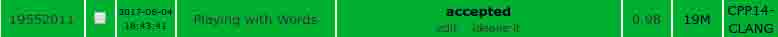
\includegraphics[scale=0.5]{assets/images/jpg/single-submission.jpg}}
  	\caption{Hasil uji coba pada situs penilaian SPOJ}
  	\label{figure:best_submission}
  \end{figure}
  
  \begin{figure}[H]
  	\centerline{ 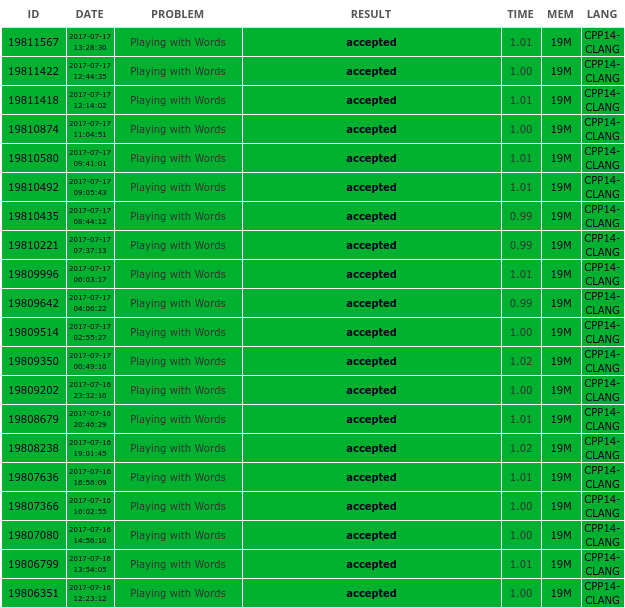
\includegraphics[scale=0.6]{assets/images/ujisubmission1.png}}
  	\caption{Hasil pengujian sebanyak 30 kali pada situs penilaian daring SPOJ (1)}
  	\label{figure:submission1}
  \end{figure}
  
  \begin{figure}[H]
  	\centerline{ 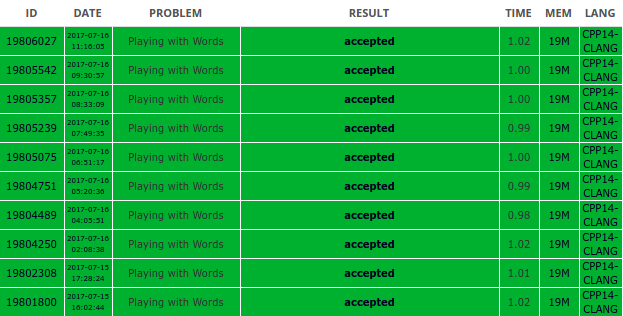
\includegraphics[scale=0.6]{assets/images/ujisubmission2.png}}
  	\caption{Hasil pengujian sebanyak 30 kali pada situs penilaian daring SPOJ (2)}
  	\label{figure:submission2}
  \end{figure}
  
  \begin{figure}[H]
  	\centerline{ 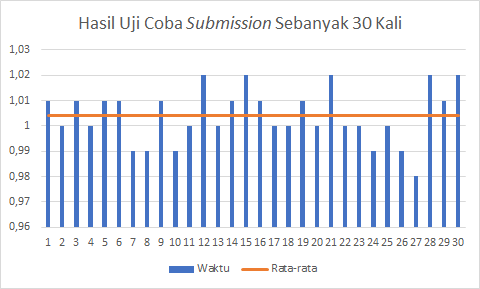
\includegraphics[scale=0.7]{assets/images/submission-chart.png}}
  	\caption{Grafik hasil uji coba pada situs SPOJ sebanyak 30 kali}
  	\label{figure:chart}
  \end{figure}
  
  \chapter{Tabel Simulasi Perhitungan Jumlah Kemungkinan \textit{String} orig1 dan orig2 pada Kasus \textit{String} ad1=c, \textit{String} ad2=n dan X=1}
  \setcounter{table}{0}
  \renewcommand{\thetable}{C.\arabic{table}}
  \renewcommand{\thefigure}{C.\arabic{figure}}
  
  % Iterasi dist = 0
  
  
  \begin{table}[H]
  	\centering
  	\begin{tabular} {|p{3cm}|p{5cm}|p{1cm}|} \hline
  		Fungsi & Perhitungan Nilai & Nilai \\ \hline
  		$ F_{(c, 0, 1)} $ & \textit{base case} & $ 1 $ \\ \hline
  		\rowcolor{LightCyan}
  		$ F_{(c, 1, 1)}  $ & $F_{(c, 0, 1)}$ & $ 1 $ \\ \hline
  	\end{tabular}\caption{Simulasi perhitungan jumlah kombinasi \textit{string} $ orig1 $ tanpa operasi \textit{replace} dengan $ dist= 0  $ pada kasus \textit{string} $ ad1=c $, \textit{string} $ ad2=n $ dan $ X=1 $}
  	\label{tab:f_2_orig1_0_1}
  \end{table}
  
  \begin{table}[H]
  	\centering
  	\begin{tabular} {|p{3cm}|p{5cm}|p{1cm}|} \hline
  		Fungsi & Perhitungan Nilai & Nilai \\ \hline
  		$ G_{(n, 0, 0)} $ & \textit{base case} & $ 0 $ \\ \hline
  		$ F_{(n, 0, 1)} $ & \textit{base case} & $ 1 $ \\ \hline
  		$ F_{(n, 0, 1)} $ & \textit{base case} & $ 1 $ \\ \hline
  		\rowcolor{LightCyan}
  		$ G_{(n, 1, 0)}  $ & $G_{(n, 0, 0)} + F_{(n, 0, 1)} + F_{(n, 0, 1)}$ & $ 2 $ \\ \hline
  	\end{tabular}\caption{Simulasi perhitungan jumlah kombinasi \textit{string} $ orig2 $ dengan operasi \textit{replace} dengan $ dist= 0  $ pada kasus \textit{string} $ ad1=c $, \textit{string} $ ad2=n $ dan $ X=1 $}
  	\label{tab:g_2_orig2_0_1}
  \end{table}
  
  \begin{table}[H]
  	\centering
  	\begin{tabular} {|p{3cm}|p{5cm}|p{1cm}|} \hline
  		Fungsi & Perhitungan Nilai & Nilai \\ \hline
  		$ G_{(c, 0, 1)} $ & \textit{base case} & $ 0 $ \\ \hline
  		$ F_{(c, 0, 2)} $ & \textit{base case} & $ 0 $ \\ \hline
  		$ F_{(c, 0, 2)} $ & \textit{base case} & $ 0 $ \\ \hline
  		\rowcolor{LightCyan}
  		$ G_{(c, 1, 1)}  $ & $G_{(c, 0, 1)} + F_{(c, 0, 2)} + F_{(c, 0, 2)}$ & $ 0 $ \\ \hline
  	\end{tabular}\caption{Simulasi perhitungan jumlah kombinasi \textit{string} $ orig1 $ dengan operasi \textit{replace} dengan $ dist= 0  $ pada kasus \textit{string} $ ad1=c $, \textit{string} $ ad2=n $ dan $ X=1 $}
  	\label{tab:g_2_orig1_0_1}
  \end{table}
  
  \begin{table}[H]
  	\centering
  	\begin{tabular} {|p{3cm}|p{5cm}|p{1cm}|} \hline
  		Fungsi & Perhitungan Nilai & Nilai \\ \hline
  		$ F_{(n, 0, 0)} $ & \textit{base case} & $ 0 $ \\ \hline
  		\rowcolor{LightCyan}
  		$ F_{(n, 1, 0)}  $ & $F_{(n, 0, 0)}$ & $ 0 $ \\ \hline
  	\end{tabular}\caption{Simulasi perhitungan jumlah kombinasi \textit{string} $ orig2 $ tanpa operasi \textit{replace} dengan $ dist= 0  $ pada kasus \textit{string} $ ad1=c $, \textit{string} $ ad2=n $ dan $ X=1 $}
  	\label{tab:f_2_orig2_0_1}
  \end{table}
  
  % Iterasi dist = 1
  
  
  \begin{table}[H]
  	\centering
  	\begin{tabular} {|p{3cm}|p{5cm}|p{1cm}|} \hline
  		Fungsi & Perhitungan Nilai & Nilai \\ \hline
  		$ F_{(c, 0, 0)} $ & \textit{base case} & $ 0 $ \\ \hline
  		\rowcolor{LightCyan}
  		$ F_{(c, 1, 0)}  $ & $F_{(c, 0, 0)}$ & $ 0 $ \\ \hline
  	\end{tabular}\caption{Simulasi perhitungan jumlah kombinasi \textit{string} $ orig1 $ tanpa operasi \textit{replace} dengan $ dist= 1  $ pada kasus \textit{string} $ ad1=c $, \textit{string} $ ad2=n $ dan $ X=1 $}
  	\label{tab:f_2_orig1_1_1}
  \end{table}
  
  \begin{table}[H]
  	\centering
  	\begin{tabular} {|p{3cm}|p{5cm}|p{1cm}|} \hline
  		Fungsi & Perhitungan Nilai & Nilai \\ \hline
  		$ G_{(n, 0, 1)} $ & \textit{base case} & $ 0 $ \\ \hline
  		$ F_{(n, 0, 2)} $ & \textit{base case} & $ 0 $ \\ \hline
  		$ F_{(n, 0, 2)} $ & \textit{base case} & $ 0 $ \\ \hline
  		\rowcolor{LightCyan}
  		$ G_{(n, 1, 1)}  $ & $G_{(n, 0, 1)} + F_{(n, 0, 2)} + F_{(n, 0, 2)}$ & $ 0 $ \\ \hline
  	\end{tabular}\caption{Simulasi perhitungan jumlah kombinasi \textit{string} $ orig2 $ dengan operasi \textit{replace} dengan $ dist= 1  $ pada kasus \textit{string} $ ad1=c $, \textit{string} $ ad2=n $ dan $ X=1 $}
  	\label{tab:g_2_orig2_1_1}
  \end{table}
  
  \begin{table}[H]
  	\centering
  	\begin{tabular} {|p{3cm}|p{5cm}|p{1cm}|} \hline
  		Fungsi & Perhitungan Nilai & Nilai \\ \hline
  		$ G_{(c, 0, 0)} $ & \textit{base case} & $ 0 $ \\ \hline
  		$ F_{(c, 0, 1)} $ & \textit{base case} & $ 1 $ \\ \hline
  		$ F_{(c, 0, 1)} $ & \textit{base case} & $ 1 $ \\ \hline
  		\rowcolor{LightCyan}
  		$ G_{(c, 1, 0)}  $ & $G_{(c, 0, 0)} + F_{(c, 0, 1)} + F_{(c, 0, 1)}$ & $ 2 $ \\ \hline
  	\end{tabular}\caption{Simulasi perhitungan jumlah kombinasi \textit{string} $ orig1 $ dengan operasi \textit{replace} dengan $ dist= 1  $ pada kasus \textit{string} $ ad1=c $, \textit{string} $ ad2=n $ dan $ X=1 $}
  	\label{tab:g_2_orig1_1_1}
  \end{table}
  
  \begin{table}[H]
  	\centering
  	\begin{tabular} {|p{3cm}|p{5cm}|p{1cm}|} \hline
  		Fungsi & Perhitungan Nilai & Nilai \\ \hline
  		$ F_{(n, 0, 1)} $ & \textit{base case} & $ 1 $ \\ \hline
  		\rowcolor{LightCyan}
  		$ F_{(n, 1, 1)}  $ & $F_{(n, 0, 1)}$ & $ 1 $ \\ \hline
  	\end{tabular}\caption{Simulasi perhitungan jumlah kombinasi \textit{string} $ orig2 $ tanpa operasi \textit{replace} dengan $ dist= 1  $ pada kasus \textit{string} $ ad1=c $, \textit{string} $ ad2=n $ dan $ X=1 $}
  	\label{tab:f_2_orig2_1_1}
  \end{table}
  
  \chapter{Tabel Simulasi Perhitungan Jumlah Kemungkinan \textit{String} orig1 dan orig2 pada Kasus \textit{String} ad1=kbenh, \textit{String} ad2=kbenh dan X=5}
  \setcounter{table}{0}
  \renewcommand{\thetable}{D.\arabic{table}}
  \renewcommand{\thefigure}{D.\arabic{figure}}
  
  % Iterasi dist = 0
  
  
  \begin{table}[H]
  	\centering
  	\begin{tabular} {|p{3cm}|p{5cm}|p{1cm}|} \hline
  		Fungsi & Perhitungan Nilai & Nilai \\ \hline
  		$ F_{(behkn, 0, 5)} $ & \textit{base case} & $ 1 $ \\ \hline
  		$ F_{(behkn, 16, 5)}  $ & $F_{(behkn, 0, 5)}$ & $ 1 $ \\ \hline
  		$ F_{(behkn, 8, 8)} $ & \textit{base case} & $ 0 $ \\ \hline
  		$ F_{(behkn, 24, 5)}  $ & $F_{(behkn, 16, 5)} + F_{(behkn, 8, 8)}$ & $ 1 $ \\ \hline
  		$ F_{(behkn, 20, 8)} $ & \textit{base case} & $ 0 $ \\ \hline
  		$ F_{(behkn, 12, 11)} $ & \textit{base case} & $ 0 $ \\ \hline
  		$ F_{(behkn, 28, 5)}  $ & $F_{(behkn, 24, 5)} + F_{(behkn, 20, 8)} + F_{(behkn, 12, 11)}$ & $ 1 $ \\ \hline
  		$ F_{(behkn, 26, 8)} $ & \textit{base case} & $ 0 $ \\ \hline
  		$ F_{(behkn, 22, 11)} $ & \textit{base case} & $ 0 $ \\ \hline
  		$ F_{(behkn, 14, 14)} $ & \textit{base case} & $ 0 $ \\ \hline
  		$ F_{(behkn, 30, 5)}  $ & $F_{(behkn, 28, 5)} + F_{(behkn, 26, 8)} + F_{(behkn, 22, 11)} + F_{(behkn, 14, 14)}$ & $ 1 $ \\ \hline
  		$ F_{(behkn, 29, 8)} $ & \textit{base case} & $ 0 $ \\ \hline
  		$ F_{(behkn, 27, 11)} $ & \textit{base case} & $ 0 $ \\ \hline
  		$ F_{(behkn, 23, 14)} $ & \textit{base case} & $ 0 $ \\ \hline
  	\end{tabular}\caption{Simulasi perhitungan jumlah kombinasi \textit{string} $ orig1 $ tanpa operasi \textit{replace} dengan $ dist= 0  $ pada kasus \textit{string} $ ad1=kbenh $, \textit{string} $ ad2=kbenh $ dan $ X=5 $}
  	\label{tab:f_3_orig1_0_1}
  \end{table}
  
  \begin{table}[H]
  	\centering
  	\begin{tabular} {|p{3cm}|p{5cm}|p{1cm}|} \hline
  		Fungsi & Perhitungan Nilai & Nilai \\ \hline  		
  		$ F_{(behkn, 15, 17)} $ & \textit{base case} & $ 0 $ \\ \hline
  		\rowcolor{LightCyan}
  		$ F_{(behkn, 31, 5)}  $ & $F_{(behkn, 30, 5)} + F_{(behkn, 29, 8)} + F_{(behkn, 27, 11)} + F_{(behkn, 23, 14)} + F_{(behkn, 15, 17)}$ & $ 1 $ \\ \hline
  	\end{tabular}\caption{Simulasi perhitungan jumlah kombinasi \textit{string} $ orig1 $ tanpa operasi \textit{replace} dengan $ dist= 0  $ pada kasus \textit{string} $ ad1=kbenh $, \textit{string} $ ad2=kbenh $ dan $ X=5 $}
  	\label{tab:f_3_orig1_0_2}
  \end{table}
  
  \begin{table}[H]
  	\centering
  	\begin{tabular} {|p{3cm}|p{5cm}|p{1cm}|} \hline
  		Fungsi & Perhitungan Nilai & Nilai \\ \hline
  		$ G_{(behkn, 0, 0)} $ & \textit{base case} & $ 0 $ \\ \hline
  		$ F_{(behkn, 0, 1)} $ & \textit{base case} & $ 0 $ \\ \hline
  		$ F_{(behkn, 0, 1)} $ & \textit{base case} & $ 0 $ \\ \hline
  		$ G_{(behkn, 16, 0)}  $ & $G_{(behkn, 0, 0)} + F_{(behkn, 0, 1)} + F_{(behkn, 0, 1)}$ & $ 0 $ \\ \hline
  		$ F_{(behkn, 0, 1)} $ & \textit{base case} & $ 0 $ \\ \hline
  		$ F_{(behkn, 16, 1)}  $ & $F_{(behkn, 0, 1)}$ & $ 0 $ \\ \hline
  		$ F_{(behkn, 16, 1)}  $ & $memoF_{(behkn, 16, 1)}$ & $ 0 $ \\ \hline
  		$ G_{(behkn, 0, 6)} $ & \textit{base case} & $ 0 $ \\ \hline
  		$ F_{(behkn, 0, 5)} $ & \textit{base case} & $ 1 $ \\ \hline
  		$ F_{(behkn, 0, 7)} $ & \textit{base case} & $ 0 $ \\ \hline
  		$ G_{(behkn, 8, 3)}  $ & $G_{(behkn, 0, 6)} + F_{(behkn, 0, 5)} + F_{(behkn, 0, 7)}$ & $ 1 $ \\ \hline
  		$ F_{(behkn, 0, 7)} $ & \textit{base case} & $ 0 $ \\ \hline
  		$ F_{(behkn, 8, 4)}  $ & $F_{(behkn, 0, 7)}$ & $ 0 $ \\ \hline
  		$ F_{(behkn, 0, 5)} $ & \textit{base case} & $ 1 $ \\ \hline
  		$ F_{(behkn, 8, 2)}  $ & $F_{(behkn, 0, 5)}$ & $ 1 $ \\ \hline
  		$ G_{(behkn, 24, 0)}  $ & $G_{(behkn, 16, 0)} + F_{(behkn, 16, 1)} + F_{(behkn, 16, 1)} + G_{(behkn, 8, 3)} + F_{(behkn, 8, 4)} + F_{(behkn, 8, 2)}$ & $ 2 $ \\ \hline
  		$ F_{(behkn, 16, 1)}  $ & $memoF_{(behkn, 16, 1)}$ & $ 0 $ \\ \hline
  		$ F_{(behkn, 8, 4)}  $ & $memoF_{(behkn, 8, 4)}$ & $ 0 $ \\ \hline
  		$ F_{(behkn, 24, 1)}  $ & $F_{(behkn, 16, 1)} + F_{(behkn, 8, 4)}$ & $ 0 $ \\ \hline
  		$ F_{(behkn, 24, 1)}  $ & $memoF_{(behkn, 24, 1)}$ & $ 0 $ \\ \hline
  		$ G_{(behkn, 16, 6)} $ & \textit{base case} & $ 0 $ \\ \hline
  		$ F_{(behkn, 0, 5)} $ & \textit{base case} & $ 1 $ \\ \hline
  		$ F_{(behkn, 16, 5)}  $ & $F_{(behkn, 0, 5)}$ & $ 1 $ \\ \hline
  		$ F_{(behkn, 16, 7)} $ & \textit{base case} & $ 0 $ \\ \hline
  	\end{tabular}\caption{Simulasi perhitungan jumlah kombinasi \textit{string} $ orig2 $ dengan operasi \textit{replace} dengan $ dist= 0  $ pada kasus \textit{string} $ ad1=kbenh $, \textit{string} $ ad2=kbenh $ dan $ X=5 $ (1)}
  	\label{tab:g_3_orig2_0_1}
  \end{table}
  \begin{table}[H]
  	\centering
  	\begin{tabular} {|p{3cm}|p{5cm}|p{1cm}|} \hline
  		Fungsi & Perhitungan Nilai & Nilai \\ \hline		
  		$ G_{(behkn, 4, 6)} $ & \textit{base case} & $ 0 $ \\ \hline
  		$ F_{(behkn, 4, 7)} $ & \textit{base case} & $ 0 $ \\ \hline
  		$ F_{(behkn, 0, 11)} $ & \textit{base case} & $ 0 $ \\ \hline
  		$ F_{(behkn, 4, 5)}  $ & $F_{(behkn, 0, 11)}$ & $ 0 $ \\ \hline
  		$ G_{(behkn, 20, 3)}  $ & $G_{(behkn, 16, 6)} + F_{(behkn, 16, 5)} + F_{(behkn, 16, 7)} + G_{(behkn, 4, 6)} + F_{(behkn, 4, 7)} + F_{(behkn, 4, 5)}$ & $ 1 $ \\ \hline
  		$ F_{(behkn, 16, 7)} $ & \textit{base case} & $ 0 $ \\ \hline
  		$ F_{(behkn, 4, 7)} $ & \textit{base case} & $ 0 $ \\ \hline
  		$ F_{(behkn, 20, 4)}  $ & $F_{(behkn, 16, 7)} + F_{(behkn, 4, 7)}$ & $ 0 $ \\ \hline
  		$ F_{(behkn, 16, 5)}  $ & $memoF_{(behkn, 16, 5)}$ & $ 1 $ \\ \hline
  		$ F_{(behkn, 4, 5)}  $ & $memoF_{(behkn, 4, 5)}$ & $ 0 $ \\ \hline
  		$ F_{(behkn, 20, 2)}  $ & $F_{(behkn, 16, 5)} + F_{(behkn, 4, 5)}$ & $ 1 $ \\ \hline
  		$ G_{(behkn, 12, 6)} $ & \textit{base case} & $ 0 $ \\ \hline
  		$ F_{(behkn, 12, 7)} $ & \textit{base case} & $ 0 $ \\ \hline
  		$ F_{(behkn, 8, 8)} $ & \textit{base case} & $ 0 $ \\ \hline
  		$ F_{(behkn, 4, 5)}  $ & $memoF_{(behkn, 4, 5)}$ & $ 0 $ \\ \hline
  		$ F_{(behkn, 12, 5)}  $ & $F_{(behkn, 8, 8)} + F_{(behkn, 4, 5)}$ & $ 0 $ \\ \hline
  		$ G_{(behkn, 28, 0)}  $ & $G_{(behkn, 24, 0)} + F_{(behkn, 24, 1)} + F_{(behkn, 24, 1)} + G_{(behkn, 20, 3)} + F_{(behkn, 20, 4)} + F_{(behkn, 20, 2)} + G_{(behkn, 12, 6)} + F_{(behkn, 12, 7)} + F_{(behkn, 12, 5)}$ & $ 4 $ \\ \hline
  		$ F_{(behkn, 24, 1)}  $ & $memoF_{(behkn, 24, 1)}$ & $ 0 $ \\ \hline
  		$ F_{(behkn, 20, 4)}  $ & $memoF_{(behkn, 20, 4)}$ & $ 0 $ \\ \hline
  		$ F_{(behkn, 12, 7)} $ & \textit{base case} & $ 0 $ \\ \hline
  		$ F_{(behkn, 28, 1)}  $ & $F_{(behkn, 24, 1)} + F_{(behkn, 20, 4)} + F_{(behkn, 12, 7)}$ & $ 0 $ \\ \hline
  	\end{tabular}\caption{Simulasi perhitungan jumlah kombinasi \textit{string} $ orig2 $ dengan operasi \textit{replace} dengan $ dist= 0  $ pada kasus \textit{string} $ ad1=kbenh $, \textit{string} $ ad2=kbenh $ dan $ X=5 $ (2)}
  	\label{tab:g_3_orig2_0_2}
  \end{table}
  \begin{table}[H]
  	\centering
  	\begin{tabular} {|p{3cm}|p{5cm}|p{1cm}|} \hline
  		Fungsi & Perhitungan Nilai & Nilai \\ \hline
  		
  		
  		$ F_{(behkn, 28, 1)}  $ & $memoF_{(behkn, 28, 1)}$ & $ 0 $ \\ \hline
  		$ G_{(behkn, 24, 6)} $ & \textit{base case} & $ 0 $ \\ \hline
  		$ F_{(behkn, 16, 5)}  $ & $memoF_{(behkn, 16, 5)}$ & $ 1 $ \\ \hline
  		$ F_{(behkn, 8, 8)} $ & \textit{base case} & $ 0 $ \\ \hline
  		$ F_{(behkn, 24, 5)}  $ & $F_{(behkn, 16, 5)} + F_{(behkn, 8, 8)}$ & $ 1 $ \\ \hline
  		$ F_{(behkn, 24, 7)} $ & \textit{base case} & $ 0 $ \\ \hline
  		$ G_{(behkn, 18, 6)} $ & \textit{base case} & $ 0 $ \\ \hline
  		$ F_{(behkn, 18, 7)} $ & \textit{base case} & $ 0 $ \\ \hline
  		$ F_{(behkn, 16, 11)} $ & \textit{base case} & $ 0 $ \\ \hline
  		$ F_{(behkn, 2, 8)} $ & \textit{base case} & $ 0 $ \\ \hline
  		$ F_{(behkn, 18, 5)}  $ & $F_{(behkn, 16, 11)} + F_{(behkn, 2, 8)}$ & $ 0 $ \\ \hline
  		$ G_{(behkn, 10, 9)} $ & \textit{base case} & $ 0 $ \\ \hline
  		$ F_{(behkn, 10, 10)} $ & \textit{base case} & $ 0 $ \\ \hline
  		$ F_{(behkn, 10, 8)} $ & \textit{base case} & $ 0 $ \\ \hline
  		$ G_{(behkn, 26, 3)}  $ & $G_{(behkn, 24, 6)} + F_{(behkn, 24, 5)} + F_{(behkn, 24, 7)} + G_{(behkn, 18, 6)} + F_{(behkn, 18, 7)} + F_{(behkn, 18, 5)} + G_{(behkn, 10, 9)} + F_{(behkn, 10, 10)} + F_{(behkn, 10, 8)}$ & $ 1 $ \\ \hline
  		$ F_{(behkn, 24, 7)} $ & \textit{base case} & $ 0 $ \\ \hline
  		$ F_{(behkn, 18, 7)} $ & \textit{base case} & $ 0 $ \\ \hline
  		$ F_{(behkn, 10, 10)} $ & \textit{base case} & $ 0 $ \\ \hline
  		$ F_{(behkn, 26, 4)}  $ & $F_{(behkn, 24, 7)} + F_{(behkn, 18, 7)} + F_{(behkn, 10, 10)}$ & $ 0 $ \\ \hline
  		$ F_{(behkn, 24, 5)}  $ & $memoF_{(behkn, 24, 5)}$ & $ 1 $ \\ \hline
  		$ F_{(behkn, 18, 5)}  $ & $memoF_{(behkn, 18, 5)}$ & $ 0 $ \\ \hline
  		$ F_{(behkn, 10, 8)} $ & \textit{base case} & $ 0 $ \\ \hline
  		$ F_{(behkn, 26, 2)}  $ & $F_{(behkn, 24, 5)} + F_{(behkn, 18, 5)} + F_{(behkn, 10, 8)}$ & $ 1 $ \\ \hline
  	\end{tabular}\caption{Simulasi perhitungan jumlah kombinasi \textit{string} $ orig2 $ dengan operasi \textit{replace} dengan $ dist= 0  $ pada kasus \textit{string} $ ad1=kbenh $, \textit{string} $ ad2=kbenh $ dan $ X=5 $ (3)}
  	\label{tab:g_3_orig2_0_3}
  \end{table}
  \begin{table}[H]
  	\centering
  	\begin{tabular} {|p{3cm}|p{5cm}|p{1cm}|} \hline
  		Fungsi & Perhitungan Nilai & Nilai \\ \hline
  		
  		$ G_{(behkn, 22, 6)} $ & \textit{base case} & $ 0 $ \\ \hline
  		$ F_{(behkn, 22, 7)} $ & \textit{base case} & $ 0 $ \\ \hline
  		$ F_{(behkn, 20, 8)} $ & \textit{base case} & $ 0 $ \\ \hline
  		$ F_{(behkn, 18, 5)}  $ & $memoF_{(behkn, 18, 5)}$ & $ 0 $ \\ \hline
  		$ F_{(behkn, 6, 11)} $ & \textit{base case} & $ 0 $ \\ \hline
  		$ F_{(behkn, 22, 5)}  $ & $F_{(behkn, 20, 8)} + F_{(behkn, 18, 5)} + F_{(behkn, 6, 11)}$ & $ 0 $ \\ \hline
  		$ G_{(behkn, 14, 9)} $ & \textit{base case} & $ 0 $ \\ \hline
  		$ F_{(behkn, 14, 10)} $ & \textit{base case} & $ 0 $ \\ \hline
  		$ F_{(behkn, 14, 8)} $ & \textit{base case} & $ 0 $ \\ \hline
  		$ G_{(behkn, 30, 0)}  $ & $G_{(behkn, 28, 0)} + F_{(behkn, 28, 1)} + F_{(behkn, 28, 1)} + G_{(behkn, 26, 3)} + F_{(behkn, 26, 4)} + F_{(behkn, 26, 2)} + G_{(behkn, 22, 6)} + F_{(behkn, 22, 7)} + F_{(behkn, 22, 5)} + G_{(behkn, 14, 9)} + F_{(behkn, 14, 10)} + F_{(behkn, 14, 8)}$ & $ 6 $ \\ \hline
  		$ F_{(behkn, 28, 1)}  $ & $memoF_{(behkn, 28, 1)}$ & $ 0 $ \\ \hline
  		$ F_{(behkn, 26, 4)}  $ & $memoF_{(behkn, 26, 4)}$ & $ 0 $ \\ \hline
  		$ F_{(behkn, 22, 7)} $ & \textit{base case} & $ 0 $ \\ \hline
  		$ F_{(behkn, 14, 10)} $ & \textit{base case} & $ 0 $ \\ \hline
  		$ F_{(behkn, 30, 1)}  $ & $F_{(behkn, 28, 1)} + F_{(behkn, 26, 4)} + F_{(behkn, 22, 7)} + F_{(behkn, 14, 10)}$ & $ 0 $ \\ \hline
  		$ F_{(behkn, 30, 1)}  $ & $memoF_{(behkn, 30, 1)}$ & $ 0 $ \\ \hline
  		$ G_{(behkn, 28, 6)} $ & \textit{base case} & $ 0 $ \\ \hline
  		$ F_{(behkn, 24, 5)}  $ & $memoF_{(behkn, 24, 5)}$ & $ 1 $ \\ \hline
  		$ F_{(behkn, 20, 8)} $ & \textit{base case} & $ 0 $ \\ \hline
  		$ F_{(behkn, 12, 11)} $ & \textit{base case} & $ 0 $ \\ \hline
  		$ F_{(behkn, 28, 5)}  $ & $F_{(behkn, 24, 5)} + F_{(behkn, 20, 8)} + F_{(behkn, 12, 11)}$ & $ 1 $ \\ \hline
  	\end{tabular}\caption{Simulasi perhitungan jumlah kombinasi \textit{string} $ orig2 $ dengan operasi \textit{replace} dengan $ dist= 0  $ pada kasus \textit{string} $ ad1=kbenh $, \textit{string} $ ad2=kbenh $ dan $ X=5 $ (4)}
  	\label{tab:g_3_orig2_0_4}
  \end{table}
  \begin{table}[H]
  	\centering
  	\begin{tabular} {|p{3cm}|p{5cm}|p{1cm}|} \hline
  		Fungsi & Perhitungan Nilai & Nilai \\ \hline
  		
  		$ F_{(behkn, 28, 7)} $ & \textit{base case} & $ 0 $ \\ \hline
  		$ G_{(behkn, 25, 6)} $ & \textit{base case} & $ 0 $ \\ \hline
  		$ F_{(behkn, 25, 7)} $ & \textit{base case} & $ 0 $ \\ \hline
  		$ F_{(behkn, 24, 11)} $ & \textit{base case} & $ 0 $ \\ \hline
  		$ F_{(behkn, 17, 8)} $ & \textit{base case} & $ 0 $ \\ \hline
  		$ F_{(behkn, 9, 11)} $ & \textit{base case} & $ 0 $ \\ \hline
  		$ F_{(behkn, 25, 5)}  $ & $F_{(behkn, 24, 11)} + F_{(behkn, 17, 8)} + F_{(behkn, 9, 11)}$ & $ 0 $ \\ \hline
  		$ G_{(behkn, 21, 9)} $ & \textit{base case} & $ 0 $ \\ \hline
  		$ F_{(behkn, 21, 10)} $ & \textit{base case} & $ 0 $ \\ \hline
  		$ F_{(behkn, 21, 8)} $ & \textit{base case} & $ 0 $ \\ \hline
  		$ G_{(behkn, 13, 12)} $ & \textit{base case} & $ 0 $ \\ \hline
  		$ F_{(behkn, 13, 13)} $ & \textit{base case} & $ 0 $ \\ \hline
  		$ F_{(behkn, 13, 11)} $ & \textit{base case} & $ 0 $ \\ \hline
  		$ G_{(behkn, 29, 3)}  $ & $G_{(behkn, 28, 6)} + F_{(behkn, 28, 5)} + F_{(behkn, 28, 7)} + G_{(behkn, 25, 6)} + F_{(behkn, 25, 7)} + F_{(behkn, 25, 5)} + G_{(behkn, 21, 9)} + F_{(behkn, 21, 10)} + F_{(behkn, 21, 8)} + G_{(behkn, 13, 12)} + F_{(behkn, 13, 13)} + F_{(behkn, 13, 11)}$ & $ 1 $ \\ \hline
  		$ F_{(behkn, 28, 7)} $ & \textit{base case} & $ 0 $ \\ \hline
  		$ F_{(behkn, 25, 7)} $ & \textit{base case} & $ 0 $ \\ \hline
  		$ F_{(behkn, 21, 10)} $ & \textit{base case} & $ 0 $ \\ \hline
  		$ F_{(behkn, 13, 13)} $ & \textit{base case} & $ 0 $ \\ \hline
  		$ F_{(behkn, 29, 4)}  $ & $F_{(behkn, 28, 7)} + F_{(behkn, 25, 7)} + F_{(behkn, 21, 10)} + F_{(behkn, 13, 13)}$ & $ 0 $ \\ \hline
  		$ F_{(behkn, 28, 5)}  $ & $memoF_{(behkn, 28, 5)}$ & $ 1 $ \\ \hline
  		$ F_{(behkn, 25, 5)}  $ & $memoF_{(behkn, 25, 5)}$ & $ 0 $ \\ \hline
  		$ F_{(behkn, 21, 8)} $ & \textit{base case} & $ 0 $ \\ \hline
  		$ F_{(behkn, 13, 11)} $ & \textit{base case} & $ 0 $ \\ \hline
  		
  		
  	\end{tabular}\caption{Simulasi perhitungan jumlah kombinasi \textit{string} $ orig2 $ dengan operasi \textit{replace} dengan $ dist= 0  $ pada kasus \textit{string} $ ad1=kbenh $, \textit{string} $ ad2=kbenh $ dan $ X=5 $ (5)}
  	\label{tab:g_3_orig2_0_5}
  \end{table}
  \begin{table}[H]
  	\centering
  	\begin{tabular} {|p{3cm}|p{5cm}|p{1cm}|} \hline
  		Fungsi & Perhitungan Nilai & Nilai \\ \hline
  		$ F_{(behkn, 27, 7)} $ & \textit{base case} & $ 0 $ \\ \hline
  		$ F_{(behkn, 26, 8)} $ & \textit{base case} & $ 0 $ \\ \hline
  		$ F_{(behkn, 25, 5)}  $ & $memoF_{(behkn, 25, 5)}$ & $ 0 $ \\ \hline
  		$ F_{(behkn, 19, 11)} $ & \textit{base case} & $ 0 $ \\ \hline
  		$ F_{(behkn, 11, 14)} $ & \textit{base case} & $ 0 $ \\ \hline
  		$ F_{(behkn, 27, 5)}  $ & $F_{(behkn, 26, 8)} + F_{(behkn, 25, 5)} + F_{(behkn, 19, 11)} + F_{(behkn, 11, 14)}$ & $ 0 $ \\ \hline
  		$ G_{(behkn, 23, 9)} $ & \textit{base case} & $ 0 $ \\ \hline
  		$ F_{(behkn, 23, 10)} $ & \textit{base case} & $ 0 $ \\ \hline
  		$ F_{(behkn, 23, 8)} $ & \textit{base case} & $ 0 $ \\ \hline
  		$ G_{(behkn, 15, 12)} $ & \textit{base case} & $ 0 $ \\ \hline
  		$ F_{(behkn, 15, 13)} $ & \textit{base case} & $ 0 $ \\ \hline
  		$ F_{(behkn, 15, 11)} $ & \textit{base case} & $ 0 $ \\ \hline
  		\rowcolor{LightCyan}
  		$ G_{(behkn, 31, 0)}  $ & $G_{(behkn, 30, 0)} + F_{(behkn, 30, 1)} + F_{(behkn, 30, 1)} + G_{(behkn, 29, 3)} + F_{(behkn, 29, 4)} + F_{(behkn, 29, 2)} + G_{(behkn, 27, 6)} + F_{(behkn, 27, 7)} + F_{(behkn, 27, 5)} + G_{(behkn, 23, 9)} + F_{(behkn, 23, 10)} + F_{(behkn, 23, 8)} + G_{(behkn, 15, 12)} + F_{(behkn, 15, 13)} + F_{(behkn, 15, 11)}$ & $ 8 $ \\ \hline
  	\end{tabular}\caption{Simulasi perhitungan jumlah kombinasi \textit{string} $ orig2 $ dengan operasi \textit{replace} dengan $ dist= 0  $ pada kasus \textit{string} $ ad1=kbenh $, \textit{string} $ ad2=kbenh $ dan $ X=5 $ (6)}
  	\label{tab:g_3_orig2_0_6}
  \end{table}
  
  \begin{table}[H]
  	\centering
  	\begin{tabular} {|p{3cm}|p{5cm}|p{1cm}|} \hline
  		Fungsi & Perhitungan Nilai & Nilai \\ \hline
  		$ G_{(behkn, 0, 5)} $ & \textit{base case} & $ 0 $ \\ \hline
  		$ F_{(behkn, 0, 6)} $ & \textit{base case} & $ 0 $ \\ \hline
  		$ F_{(behkn, 0, 6)} $ & \textit{base case} & $ 0 $ \\ \hline
  		$ G_{(behkn, 16, 5)}  $ & $G_{(behkn, 0, 5)} + F_{(behkn, 0, 6)} + F_{(behkn, 0, 6)}$ & $ 0 $ \\ \hline
  		$ F_{(behkn, 16, 6)} $ & \textit{base case} & $ 0 $ \\ \hline
  		$ F_{(behkn, 16, 6)} $ & \textit{base case} & $ 0 $ \\ \hline
  		$ G_{(behkn, 8, 8)} $ & \textit{base case} & $ 0 $ \\ \hline
  		$ F_{(behkn, 8, 9)} $ & \textit{base case} & $ 0 $ \\ \hline
  		$ F_{(behkn, 8, 7)} $ & \textit{base case} & $ 0 $ \\ \hline
  		$ G_{(behkn, 24, 5)}  $ & $G_{(behkn, 16, 5)} + F_{(behkn, 16, 6)} + F_{(behkn, 16, 6)} + G_{(behkn, 8, 8)} + F_{(behkn, 8, 9)} + F_{(behkn, 8, 7)}$ & $ 0 $ \\ \hline
  		$ F_{(behkn, 24, 6)} $ & \textit{base case} & $ 0 $ \\ \hline
  		$ F_{(behkn, 24, 6)} $ & \textit{base case} & $ 0 $ \\ \hline
  		$ G_{(behkn, 20, 8)} $ & \textit{base case} & $ 0 $ \\ \hline
  		$ F_{(behkn, 20, 9)} $ & \textit{base case} & $ 0 $ \\ \hline
  		$ F_{(behkn, 20, 7)} $ & \textit{base case} & $ 0 $ \\ \hline
  		$ G_{(behkn, 12, 11)} $ & \textit{base case} & $ 0 $ \\ \hline
  		$ F_{(behkn, 12, 12)} $ & \textit{base case} & $ 0 $ \\ \hline
  		$ F_{(behkn, 12, 10)} $ & \textit{base case} & $ 0 $ \\ \hline
  		$ G_{(behkn, 28, 5)}  $ & $G_{(behkn, 24, 5)} + F_{(behkn, 24, 6)} + F_{(behkn, 24, 6)} + G_{(behkn, 20, 8)} + F_{(behkn, 20, 9)} + F_{(behkn, 20, 7)} + G_{(behkn, 12, 11)} + F_{(behkn, 12, 12)} + F_{(behkn, 12, 10)}$ & $ 0 $ \\ \hline
  		$ F_{(behkn, 28, 6)} $ & \textit{base case} & $ 0 $ \\ \hline
  		$ F_{(behkn, 28, 6)} $ & \textit{base case} & $ 0 $ \\ \hline
  	\end{tabular}\caption{Simulasi perhitungan jumlah kombinasi \textit{string} $ orig1 $ dengan operasi \textit{replace} dengan $ dist= 0  $ pada kasus \textit{string} $ ad1=kbenh $, \textit{string} $ ad2=kbenh $ dan $ X=5 $ (1)}
  	\label{tab:g_3_orig1_0_1}
  \end{table}
  \begin{table}[H]
  	\centering
  	\begin{tabular} {|p{3cm}|p{5cm}|p{1cm}|} \hline
  		Fungsi & Perhitungan Nilai & Nilai \\ \hline		
  		$ G_{(behkn, 26, 8)} $ & \textit{base case} & $ 0 $ \\ \hline
  		$ F_{(behkn, 26, 9)} $ & \textit{base case} & $ 0 $ \\ \hline
  		$ F_{(behkn, 26, 7)} $ & \textit{base case} & $ 0 $ \\ \hline
  		$ G_{(behkn, 22, 11)} $ & \textit{base case} & $ 0 $ \\ \hline
  		$ F_{(behkn, 22, 12)} $ & \textit{base case} & $ 0 $ \\ \hline
  		$ F_{(behkn, 22, 10)} $ & \textit{base case} & $ 0 $ \\ \hline
  		$ G_{(behkn, 14, 14)} $ & \textit{base case} & $ 0 $ \\ \hline
  		$ F_{(behkn, 14, 15)} $ & \textit{base case} & $ 0 $ \\ \hline
  		$ F_{(behkn, 14, 13)} $ & \textit{base case} & $ 0 $ \\ \hline
  		$ G_{(behkn, 30, 5)}  $ & $G_{(behkn, 28, 5)} + F_{(behkn, 28, 6)} + F_{(behkn, 28, 6)} + G_{(behkn, 26, 8)} + F_{(behkn, 26, 9)} + F_{(behkn, 26, 7)} + G_{(behkn, 22, 11)} + F_{(behkn, 22, 12)} + F_{(behkn, 22, 10)} + G_{(behkn, 14, 14)} + F_{(behkn, 14, 15)} + F_{(behkn, 14, 13)}$ & $ 0 $ \\ \hline
  		$ F_{(behkn, 30, 6)} $ & \textit{base case} & $ 0 $ \\ \hline
  		$ F_{(behkn, 30, 6)} $ & \textit{base case} & $ 0 $ \\ \hline
  		$ G_{(behkn, 29, 8)} $ & \textit{base case} & $ 0 $ \\ \hline
  		$ F_{(behkn, 29, 9)} $ & \textit{base case} & $ 0 $ \\ \hline
  		$ F_{(behkn, 29, 7)} $ & \textit{base case} & $ 0 $ \\ \hline
  		$ G_{(behkn, 27, 11)} $ & \textit{base case} & $ 0 $ \\ \hline
  		$ F_{(behkn, 27, 12)} $ & \textit{base case} & $ 0 $ \\ \hline
  		$ F_{(behkn, 27, 10)} $ & \textit{base case} & $ 0 $ \\ \hline
  		$ G_{(behkn, 23, 14)} $ & \textit{base case} & $ 0 $ \\ \hline
  		$ F_{(behkn, 23, 15)} $ & \textit{base case} & $ 0 $ \\ \hline
  		$ F_{(behkn, 23, 13)} $ & \textit{base case} & $ 0 $ \\ \hline
  		$ G_{(behkn, 15, 17)} $ & \textit{base case} & $ 0 $ \\ \hline
  	\end{tabular}\caption{Simulasi perhitungan jumlah kombinasi \textit{string} $ orig1 $ dengan operasi \textit{replace} dengan $ dist= 0  $ pada kasus \textit{string} $ ad1=kbenh $, \textit{string} $ ad2=kbenh $ dan $ X=5 $ (2)}
  	\label{tab:g_3_orig1_0_2}
  \end{table}
  \begin{table}[H]
  	\centering
  	\begin{tabular} {|p{3cm}|p{5cm}|p{1cm}|} \hline
  		Fungsi & Perhitungan Nilai & Nilai \\ \hline
  		
  		$ F_{(behkn, 15, 18)} $ & \textit{base case} & $ 0 $ \\ \hline
  		$ F_{(behkn, 15, 16)} $ & \textit{base case} & $ 0 $ \\ \hline
  		\rowcolor{LightCyan}
  		$ G_{(behkn, 31, 5)}  $ & $G_{(behkn, 30, 5)} + F_{(behkn, 30, 6)} + F_{(behkn, 30, 6)} + G_{(behkn, 29, 8)} + F_{(behkn, 29, 9)} + F_{(behkn, 29, 7)} + G_{(behkn, 27, 11)} + F_{(behkn, 27, 12)} + F_{(behkn, 27, 10)} + G_{(behkn, 23, 14)} + F_{(behkn, 23, 15)} + F_{(behkn, 23, 13)} + G_{(behkn, 15, 17)} + F_{(behkn, 15, 18)} + F_{(behkn, 15, 16)}$ & $ 0 $ \\ \hline
  	\end{tabular}\caption{Simulasi perhitungan jumlah kombinasi \textit{string} $ orig1 $ dengan operasi \textit{replace} dengan $ dist= 0  $ pada kasus \textit{string} $ ad1=kbenh $, \textit{string} $ ad2=kbenh $ dan $ X=5 $ (3)}
  	\label{tab:g_3_orig1_0_3}
  \end{table}
  
  \begin{table}[H]
  	\centering
  	\begin{tabular} {|p{3cm}|p{5cm}|p{1cm}|} \hline
  		Fungsi & Perhitungan Nilai & Nilai \\ \hline
  		$ F_{(behkn, 0, 0)} $ & \textit{base case} & $ 0 $ \\ \hline
  		$ F_{(behkn, 16, 0)}  $ & $F_{(behkn, 0, 0)}$ & $ 0 $ \\ \hline
  		$ F_{(behkn, 0, 6)} $ & \textit{base case} & $ 0 $ \\ \hline
  		$ F_{(behkn, 8, 3)}  $ & $F_{(behkn, 0, 6)}$ & $ 0 $ \\ \hline
  		$ F_{(behkn, 24, 0)}  $ & $F_{(behkn, 16, 0)} + F_{(behkn, 8, 3)}$ & $ 0 $ \\ \hline
  		$ F_{(behkn, 16, 6)} $ & \textit{base case} & $ 0 $ \\ \hline
  		$ F_{(behkn, 4, 6)} $ & \textit{base case} & $ 0 $ \\ \hline
  		$ F_{(behkn, 20, 3)}  $ & $F_{(behkn, 16, 6)} + F_{(behkn, 4, 6)}$ & $ 0 $ \\ \hline
  		$ F_{(behkn, 12, 6)} $ & \textit{base case} & $ 0 $ \\ \hline
  		$ F_{(behkn, 28, 0)}  $ & $F_{(behkn, 24, 0)} + F_{(behkn, 20, 3)} + F_{(behkn, 12, 6)}$ & $ 0 $ \\ \hline
  		$ F_{(behkn, 24, 6)} $ & \textit{base case} & $ 0 $ \\ \hline
  		$ F_{(behkn, 18, 6)} $ & \textit{base case} & $ 0 $ \\ \hline
  		$ F_{(behkn, 10, 9)} $ & \textit{base case} & $ 0 $ \\ \hline
  		$ F_{(behkn, 26, 3)}  $ & $F_{(behkn, 24, 6)} + F_{(behkn, 18, 6)} + F_{(behkn, 10, 9)}$ & $ 0 $ \\ \hline
  		$ F_{(behkn, 22, 6)} $ & \textit{base case} & $ 0 $ \\ \hline
  		$ F_{(behkn, 14, 9)} $ & \textit{base case} & $ 0 $ \\ \hline
  		$ F_{(behkn, 30, 0)}  $ & $F_{(behkn, 28, 0)} + F_{(behkn, 26, 3)} + F_{(behkn, 22, 6)} + F_{(behkn, 14, 9)}$ & $ 0 $ \\ \hline
  		$ F_{(behkn, 28, 6)} $ & \textit{base case} & $ 0 $ \\ \hline
  		$ F_{(behkn, 25, 6)} $ & \textit{base case} & $ 0 $ \\ \hline
  		$ F_{(behkn, 21, 9)} $ & \textit{base case} & $ 0 $ \\ \hline
  		$ F_{(behkn, 13, 12)} $ & \textit{base case} & $ 0 $ \\ \hline
  		$ F_{(behkn, 29, 3)}  $ & $F_{(behkn, 28, 6)} + F_{(behkn, 25, 6)} + F_{(behkn, 21, 9)} + F_{(behkn, 13, 12)}$ & $ 0 $ \\ \hline
  	\end{tabular}\caption{Simulasi perhitungan jumlah kombinasi \textit{string} $ orig2 $ tanpa operasi \textit{replace} dengan $ dist= 0  $ pada kasus \textit{string} $ ad1=kbenh $, \textit{string} $ ad2=kbenh $ dan $ X=5 $ (1)}
  	\label{tab:f_3_orig2_0_1}
  \end{table}
  \begin{table}[H]
  	\centering
  	\begin{tabular} {|p{3cm}|p{5cm}|p{1cm}|} \hline
  		Fungsi & Perhitungan Nilai & Nilai \\ \hline		
  		
  		$ F_{(behkn, 27, 6)} $ & \textit{base case} & $ 0 $ \\ \hline
  		$ F_{(behkn, 23, 9)} $ & \textit{base case} & $ 0 $ \\ \hline
  		$ F_{(behkn, 15, 12)} $ & \textit{base case} & $ 0 $ \\ \hline
  		\rowcolor{LightCyan}
  		$ F_{(behkn, 31, 0)}  $ & $F_{(behkn, 30, 0)} + F_{(behkn, 29, 3)} + F_{(behkn, 27, 6)} + F_{(behkn, 23, 9)} + F_{(behkn, 15, 12)}$ & $ 0 $ \\ \hline
  	\end{tabular}\caption{Simulasi perhitungan jumlah kombinasi \textit{string} $ orig2 $ tanpa operasi \textit{replace} dengan $ dist= 0  $ pada kasus \textit{string} $ ad1=kbenh $, \textit{string} $ ad2=kbenh $ dan $ X=5 $ (2)}
  	\label{tab:f_3_orig2_0_2}
  \end{table}
  
  
  % -----------------------------------------------------
  % -----------------------------------------------------
  % -----------------------------------------------------
  % -----------------------------------------------------
  % -----------------------------------------------------
  % -----------------------------------------------------
  % -----------------------------------------------------
  % -----------------------------------------------------
  % -----------------------------------------------------
  % -----------------------------------------------------
  % -----------------------------------------------------
  % -----------------------------------------------------
  % -----------------------------------------------------
  % -----------------------------------------------------
  % -----------------------------------------------------
  % -----------------------------------------------------
  % -----------------------------------------------------
  % -----------------------------------------------------
  % -----------------------------------------------------
  % -----------------------------------------------------
  % -----------------------------------------------------
  % -----------------------------------------------------
  % -----------------------------------------------------
  % -----------------------------------------------------
  % -----------------------------------------------------
  % -----------------------------------------------------
  % -----------------------------------------------------
  % -----------------------------------------------------
  % -----------------------------------------------------
  % -----------------------------------------------------
  % -----------------------------------------------------
  % -----------------------------------------------------
  % -----------------------------------------------------
  
  % Iterasi dist = 1
  
  
  \begin{table}[H]
  	\centering
  	\begin{tabular} {|p{3cm}|p{5cm}|p{1cm}|} \hline
  		Fungsi & Perhitungan Nilai & Nilai \\ \hline
  		$ F_{(behkn, 0, 4)} $ & \textit{base case} & $ 0 $ \\ \hline
  		$ F_{(behkn, 16, 4)}  $ & $F_{(behkn, 0, 4)}$ & $ 0 $ \\ \hline
  		$ F_{(behkn, 8, 7)} $ & \textit{base case} & $ 0 $ \\ \hline
  		$ F_{(behkn, 24, 4)}  $ & $F_{(behkn, 16, 4)} + F_{(behkn, 8, 7)}$ & $ 0 $ \\ \hline
  		$ F_{(behkn, 20, 7)} $ & \textit{base case} & $ 0 $ \\ \hline
  		$ F_{(behkn, 12, 10)} $ & \textit{base case} & $ 0 $ \\ \hline
  		$ F_{(behkn, 28, 4)}  $ & $F_{(behkn, 24, 4)} + F_{(behkn, 20, 7)} + F_{(behkn, 12, 10)}$ & $ 0 $ \\ \hline
  		$ F_{(behkn, 26, 7)} $ & \textit{base case} & $ 0 $ \\ \hline
  		$ F_{(behkn, 22, 10)} $ & \textit{base case} & $ 0 $ \\ \hline
  		$ F_{(behkn, 14, 13)} $ & \textit{base case} & $ 0 $ \\ \hline
  		$ F_{(behkn, 30, 4)}  $ & $F_{(behkn, 28, 4)} + F_{(behkn, 26, 7)} + F_{(behkn, 22, 10)} + F_{(behkn, 14, 13)}$ & $ 0 $ \\ \hline
  		$ F_{(behkn, 29, 7)} $ & \textit{base case} & $ 0 $ \\ \hline
  		$ F_{(behkn, 27, 10)} $ & \textit{base case} & $ 0 $ \\ \hline
  		$ F_{(behkn, 23, 13)} $ & \textit{base case} & $ 0 $ \\ \hline
  		$ F_{(behkn, 15, 16)} $ & \textit{base case} & $ 0 $ \\ \hline
  		\rowcolor{LightCyan}
  		$ F_{(behkn, 31, 4)}  $ & $F_{(behkn, 30, 4)} + F_{(behkn, 29, 7)} + F_{(behkn, 27, 10)} + F_{(behkn, 23, 13)} + F_{(behkn, 15, 16)}$ & $ 0 $ \\ \hline
  	\end{tabular}\caption{Simulasi perhitungan jumlah kombinasi \textit{string} $ orig1 $ tanpa operasi \textit{replace} dengan $ dist= 1  $ pada kasus \textit{string} $ ad1=kbenh $, \textit{string} $ ad2=kbenh $ dan $ X=5 $}
  	\label{tab:f_3_orig1_1_1}
  \end{table}
  
  \begin{table}[H]
  	\centering
  	\begin{tabular} {|p{3cm}|p{5cm}|p{1cm}|} \hline
  		Fungsi & Perhitungan Nilai & Nilai \\ \hline
  		$ G_{(behkn, 0, 1)} $ & \textit{base case} & $ 0 $ \\ \hline
  		$ F_{(behkn, 0, 2)} $ & \textit{base case} & $ 0 $ \\ \hline
  		$ F_{(behkn, 0, 2)} $ & \textit{base case} & $ 0 $ \\ \hline
  		$ G_{(behkn, 16, 1)}  $ & $G_{(behkn, 0, 1)} + F_{(behkn, 0, 2)} + F_{(behkn, 0, 2)}$ & $ 0 $ \\ \hline
  		$ F_{(behkn, 0, 2)} $ & \textit{base case} & $ 0 $ \\ \hline
  		$ F_{(behkn, 16, 2)}  $ & $F_{(behkn, 0, 2)}$ & $ 0 $ \\ \hline
  		$ F_{(behkn, 16, 2)}  $ & $memoF_{(behkn, 16, 2)}$ & $ 0 $ \\ \hline
  		$ G_{(behkn, 0, 7)} $ & \textit{base case} & $ 0 $ \\ \hline
  		$ F_{(behkn, 0, 6)} $ & \textit{base case} & $ 0 $ \\ \hline
  		$ F_{(behkn, 0, 8)} $ & \textit{base case} & $ 0 $ \\ \hline
  		$ G_{(behkn, 8, 4)}  $ & $G_{(behkn, 0, 7)} + F_{(behkn, 0, 6)} + F_{(behkn, 0, 8)}$ & $ 0 $ \\ \hline
  		$ F_{(behkn, 0, 8)} $ & \textit{base case} & $ 0 $ \\ \hline
  		$ F_{(behkn, 8, 5)}  $ & $F_{(behkn, 0, 8)}$ & $ 0 $ \\ \hline
  		$ F_{(behkn, 8, 3)}  $ & $memoF_{(behkn, 8, 3)}$ & $ 0 $ \\ \hline
  		$ G_{(behkn, 24, 1)}  $ & $G_{(behkn, 16, 1)} + F_{(behkn, 16, 2)} + F_{(behkn, 16, 2)} + G_{(behkn, 8, 4)} + F_{(behkn, 8, 5)} + F_{(behkn, 8, 3)}$ & $ 0 $ \\ \hline
  		$ F_{(behkn, 16, 2)}  $ & $memoF_{(behkn, 16, 2)}$ & $ 0 $ \\ \hline
  		$ F_{(behkn, 8, 5)}  $ & $memoF_{(behkn, 8, 5)}$ & $ 0 $ \\ \hline
  		$ F_{(behkn, 24, 2)}  $ & $F_{(behkn, 16, 2)} + F_{(behkn, 8, 5)}$ & $ 0 $ \\ \hline
  		$ F_{(behkn, 24, 2)}  $ & $memoF_{(behkn, 24, 2)}$ & $ 0 $ \\ \hline
  		$ G_{(behkn, 16, 7)} $ & \textit{base case} & $ 0 $ \\ \hline
  		$ F_{(behkn, 16, 6)} $ & \textit{base case} & $ 0 $ \\ \hline
  		$ F_{(behkn, 16, 8)} $ & \textit{base case} & $ 0 $ \\ \hline
  	\end{tabular}\caption{Simulasi perhitungan jumlah kombinasi \textit{string} $ orig2 $ dengan operasi \textit{replace} dengan $ dist= 1  $ pada kasus \textit{string} $ ad1=kbenh $, \textit{string} $ ad2=kbenh $ dan $ X=5 $ (1)}
  	\label{tab:g_3_orig2_1_1}
  \end{table}
  \begin{table}[H]
  	\centering
  	\begin{tabular} {|p{3cm}|p{5cm}|p{1cm}|} \hline
  		Fungsi & Perhitungan Nilai & Nilai \\ \hline				
  		$ G_{(behkn, 4, 7)} $ & \textit{base case} & $ 0 $ \\ \hline
  		$ F_{(behkn, 4, 8)} $ & \textit{base case} & $ 0 $ \\ \hline
  		$ F_{(behkn, 4, 6)} $ & \textit{base case} & $ 0 $ \\ \hline
  		$ G_{(behkn, 20, 4)}  $ & $G_{(behkn, 16, 7)} + F_{(behkn, 16, 6)} + F_{(behkn, 16, 8)} + G_{(behkn, 4, 7)} + F_{(behkn, 4, 8)} + F_{(behkn, 4, 6)}$ & $ 0 $ \\ \hline
  		$ F_{(behkn, 16, 8)} $ & \textit{base case} & $ 0 $ \\ \hline
  		$ F_{(behkn, 4, 8)} $ & \textit{base case} & $ 0 $ \\ \hline
  		$ F_{(behkn, 20, 5)}  $ & $F_{(behkn, 16, 8)} + F_{(behkn, 4, 8)}$ & $ 0 $ \\ \hline
  		$ F_{(behkn, 20, 3)}  $ & $memoF_{(behkn, 20, 3)}$ & $ 0 $ \\ \hline
  		$ G_{(behkn, 12, 7)} $ & \textit{base case} & $ 0 $ \\ \hline
  		$ F_{(behkn, 12, 8)} $ & \textit{base case} & $ 0 $ \\ \hline
  		$ F_{(behkn, 12, 6)} $ & \textit{base case} & $ 0 $ \\ \hline
  		$ G_{(behkn, 28, 1)}  $ & $G_{(behkn, 24, 1)} + F_{(behkn, 24, 2)} + F_{(behkn, 24, 2)} + G_{(behkn, 20, 4)} + F_{(behkn, 20, 5)} + F_{(behkn, 20, 3)} + G_{(behkn, 12, 7)} + F_{(behkn, 12, 8)} + F_{(behkn, 12, 6)}$ & $ 0 $ \\ \hline
  		$ F_{(behkn, 24, 2)}  $ & $memoF_{(behkn, 24, 2)}$ & $ 0 $ \\ \hline
  		$ F_{(behkn, 20, 5)}  $ & $memoF_{(behkn, 20, 5)}$ & $ 0 $ \\ \hline
  		$ F_{(behkn, 12, 8)} $ & \textit{base case} & $ 0 $ \\ \hline
  		$ F_{(behkn, 28, 2)}  $ & $F_{(behkn, 24, 2)} + F_{(behkn, 20, 5)} + F_{(behkn, 12, 8)}$ & $ 0 $ \\ \hline
  		$ F_{(behkn, 28, 2)}  $ & $memoF_{(behkn, 28, 2)}$ & $ 0 $ \\ \hline
  		$ G_{(behkn, 24, 7)} $ & \textit{base case} & $ 0 $ \\ \hline
  		$ F_{(behkn, 24, 6)} $ & \textit{base case} & $ 0 $ \\ \hline
  		$ F_{(behkn, 24, 8)} $ & \textit{base case} & $ 0 $ \\ \hline
  		$ G_{(behkn, 18, 7)} $ & \textit{base case} & $ 0 $ \\ \hline
  	\end{tabular}\caption{Simulasi perhitungan jumlah kombinasi \textit{string} $ orig2 $ dengan operasi \textit{replace} dengan $ dist= 1  $ pada kasus \textit{string} $ ad1=kbenh $, \textit{string} $ ad2=kbenh $ dan $ X=5 $ (2)}
  	\label{tab:g_3_orig2_1_2}
  \end{table}
  \begin{table}[H]
  	\centering
  	\begin{tabular} {|p{3cm}|p{5cm}|p{1cm}|} \hline
  		Fungsi & Perhitungan Nilai & Nilai \\ \hline				
  		$ F_{(behkn, 18, 8)} $ & \textit{base case} & $ 0 $ \\ \hline
  		$ F_{(behkn, 18, 6)} $ & \textit{base case} & $ 0 $ \\ \hline
  		$ G_{(behkn, 10, 10)} $ & \textit{base case} & $ 0 $ \\ \hline
  		$ F_{(behkn, 10, 11)} $ & \textit{base case} & $ 0 $ \\ \hline
  		$ F_{(behkn, 10, 9)} $ & \textit{base case} & $ 0 $ \\ \hline
  		$ G_{(behkn, 26, 4)}  $ & $G_{(behkn, 24, 7)} + F_{(behkn, 24, 6)} + F_{(behkn, 24, 8)} + G_{(behkn, 18, 7)} + F_{(behkn, 18, 8)} + F_{(behkn, 18, 6)} + G_{(behkn, 10, 10)} + F_{(behkn, 10, 11)} + F_{(behkn, 10, 9)}$ & $ 0 $ \\ \hline
  		$ F_{(behkn, 24, 8)} $ & \textit{base case} & $ 0 $ \\ \hline
  		$ F_{(behkn, 18, 8)} $ & \textit{base case} & $ 0 $ \\ \hline
  		$ F_{(behkn, 10, 11)} $ & \textit{base case} & $ 0 $ \\ \hline
  		$ F_{(behkn, 26, 5)}  $ & $F_{(behkn, 24, 8)} + F_{(behkn, 18, 8)} + F_{(behkn, 10, 11)}$ & $ 0 $ \\ \hline
  		$ F_{(behkn, 26, 3)}  $ & $memoF_{(behkn, 26, 3)}$ & $ 0 $ \\ \hline
  		$ G_{(behkn, 22, 7)} $ & \textit{base case} & $ 0 $ \\ \hline
  		$ F_{(behkn, 22, 8)} $ & \textit{base case} & $ 0 $ \\ \hline
  		$ F_{(behkn, 22, 6)} $ & \textit{base case} & $ 0 $ \\ \hline
  		$ G_{(behkn, 14, 10)} $ & \textit{base case} & $ 0 $ \\ \hline
  		$ F_{(behkn, 14, 11)} $ & \textit{base case} & $ 0 $ \\ \hline
  		$ F_{(behkn, 14, 9)} $ & \textit{base case} & $ 0 $ \\ \hline
  		$ G_{(behkn, 30, 1)}  $ & $G_{(behkn, 28, 1)} + F_{(behkn, 28, 2)} + F_{(behkn, 28, 2)} + G_{(behkn, 26, 4)} + F_{(behkn, 26, 5)} + F_{(behkn, 26, 3)} + G_{(behkn, 22, 7)} + F_{(behkn, 22, 8)} + F_{(behkn, 22, 6)} + G_{(behkn, 14, 10)} + F_{(behkn, 14, 11)} + F_{(behkn, 14, 9)}$ & $ 0 $ \\ \hline
  	\end{tabular}\caption{Simulasi perhitungan jumlah kombinasi \textit{string} $ orig2 $ dengan operasi \textit{replace} dengan $ dist= 1  $ pada kasus \textit{string} $ ad1=kbenh $, \textit{string} $ ad2=kbenh $ dan $ X=5 $ (3)}
  	\label{tab:g_3_orig2_1_3}
  \end{table}
  \begin{table}[H]
  	\centering
  	\begin{tabular} {|p{3cm}|p{5cm}|p{1cm}|} \hline
  		Fungsi & Perhitungan Nilai & Nilai \\ \hline		
  		
  		$ F_{(behkn, 28, 2)}  $ & $memoF_{(behkn, 28, 2)}$ & $ 0 $ \\ \hline
  		$ F_{(behkn, 26, 5)}  $ & $memoF_{(behkn, 26, 5)}$ & $ 0 $ \\ \hline
  		$ F_{(behkn, 22, 8)} $ & \textit{base case} & $ 0 $ \\ \hline
  		$ F_{(behkn, 14, 11)} $ & \textit{base case} & $ 0 $ \\ \hline
  		$ F_{(behkn, 30, 2)}  $ & $F_{(behkn, 28, 2)} + F_{(behkn, 26, 5)} + F_{(behkn, 22, 8)} + F_{(behkn, 14, 11)}$ & $ 0 $ \\ \hline
  		$ F_{(behkn, 30, 2)}  $ & $memoF_{(behkn, 30, 2)}$ & $ 0 $ \\ \hline
  		$ G_{(behkn, 28, 7)} $ & \textit{base case} & $ 0 $ \\ \hline
  		$ F_{(behkn, 28, 6)} $ & \textit{base case} & $ 0 $ \\ \hline
  		$ F_{(behkn, 28, 8)} $ & \textit{base case} & $ 0 $ \\ \hline
  		$ G_{(behkn, 25, 7)} $ & \textit{base case} & $ 0 $ \\ \hline
  		$ F_{(behkn, 25, 8)} $ & \textit{base case} & $ 0 $ \\ \hline
  		$ F_{(behkn, 25, 6)} $ & \textit{base case} & $ 0 $ \\ \hline
  		$ G_{(behkn, 21, 10)} $ & \textit{base case} & $ 0 $ \\ \hline
  		$ F_{(behkn, 21, 11)} $ & \textit{base case} & $ 0 $ \\ \hline
  		$ F_{(behkn, 21, 9)} $ & \textit{base case} & $ 0 $ \\ \hline
  		$ G_{(behkn, 13, 13)} $ & \textit{base case} & $ 0 $ \\ \hline
  		$ F_{(behkn, 13, 14)} $ & \textit{base case} & $ 0 $ \\ \hline
  		$ F_{(behkn, 13, 12)} $ & \textit{base case} & $ 0 $ \\ \hline
  		$ G_{(behkn, 29, 4)}  $ & $G_{(behkn, 28, 7)} + F_{(behkn, 28, 6)} + F_{(behkn, 28, 8)} + G_{(behkn, 25, 7)} + F_{(behkn, 25, 8)} + F_{(behkn, 25, 6)} + G_{(behkn, 21, 10)} + F_{(behkn, 21, 11)} + F_{(behkn, 21, 9)} + G_{(behkn, 13, 13)} + F_{(behkn, 13, 14)} + F_{(behkn, 13, 12)}$ & $ 0 $ \\ \hline
  		$ F_{(behkn, 28, 8)} $ & \textit{base case} & $ 0 $ \\ \hline
  		$ F_{(behkn, 25, 8)} $ & \textit{base case} & $ 0 $ \\ \hline
  		$ F_{(behkn, 21, 11)} $ & \textit{base case} & $ 0 $ \\ \hline
  		
  	\end{tabular}\caption{Simulasi perhitungan jumlah kombinasi \textit{string} $ orig2 $ dengan operasi \textit{replace} dengan $ dist= 1  $ pada kasus \textit{string} $ ad1=kbenh $, \textit{string} $ ad2=kbenh $ dan $ X=5 $ (4)}
  	\label{tab:g_3_orig2_1_4}
  \end{table}
  \begin{table}[H]
  	\centering
  	\begin{tabular} {|p{3cm}|p{5cm}|p{1cm}|} \hline
  		Fungsi & Perhitungan Nilai & Nilai \\ \hline		
  		$ F_{(behkn, 13, 14)} $ & \textit{base case} & $ 0 $ \\ \hline
  		$ F_{(behkn, 29, 5)}  $ & $F_{(behkn, 28, 8)} + F_{(behkn, 25, 8)} + F_{(behkn, 21, 11)} + F_{(behkn, 13, 14)}$ & $ 0 $ \\ \hline
  		$ F_{(behkn, 29, 3)}  $ & $memoF_{(behkn, 29, 3)}$ & $ 0 $ \\ \hline
  		$ G_{(behkn, 27, 7)} $ & \textit{base case} & $ 0 $ \\ \hline
  		$ F_{(behkn, 27, 8)} $ & \textit{base case} & $ 0 $ \\ \hline
  		$ F_{(behkn, 27, 6)} $ & \textit{base case} & $ 0 $ \\ \hline
  		$ G_{(behkn, 23, 10)} $ & \textit{base case} & $ 0 $ \\ \hline
  		$ F_{(behkn, 23, 11)} $ & \textit{base case} & $ 0 $ \\ \hline
  		$ F_{(behkn, 23, 9)} $ & \textit{base case} & $ 0 $ \\ \hline
  		$ G_{(behkn, 15, 13)} $ & \textit{base case} & $ 0 $ \\ \hline
  		$ F_{(behkn, 15, 14)} $ & \textit{base case} & $ 0 $ \\ \hline
  		$ F_{(behkn, 15, 12)} $ & \textit{base case} & $ 0 $ \\ \hline
  		\rowcolor{LightCyan}
  		$ G_{(behkn, 31, 1)}  $ & $G_{(behkn, 30, 1)} + F_{(behkn, 30, 2)} + F_{(behkn, 30, 2)} + G_{(behkn, 29, 4)} + F_{(behkn, 29, 5)} + F_{(behkn, 29, 3)} + G_{(behkn, 27, 7)} + F_{(behkn, 27, 8)} + F_{(behkn, 27, 6)} + G_{(behkn, 23, 10)} + F_{(behkn, 23, 11)} + F_{(behkn, 23, 9)} + G_{(behkn, 15, 13)} + F_{(behkn, 15, 14)} + F_{(behkn, 15, 12)}$ & $ 0 $ \\ \hline
  	\end{tabular}\caption{Simulasi perhitungan jumlah kombinasi \textit{string} $ orig2 $ dengan operasi \textit{replace} dengan $ dist= 1  $ pada kasus \textit{string} $ ad1=kbenh $, \textit{string} $ ad2=kbenh $ dan $ X=5 $ (5)}
  	\label{tab:g_3_orig2_1_5}
  \end{table}
  
  \begin{table}[H]
  	\centering
  	\begin{tabular} {|p{3cm}|p{5cm}|p{1cm}|} \hline
  		Fungsi & Perhitungan Nilai & Nilai \\ \hline
  		$ G_{(behkn, 0, 4)} $ & \textit{base case} & $ 0 $ \\ \hline
  		$ F_{(behkn, 0, 5)} $ & \textit{base case} & $ 1 $ \\ \hline
  		$ F_{(behkn, 0, 5)} $ & \textit{base case} & $ 1 $ \\ \hline
  		$ G_{(behkn, 16, 4)}  $ & $G_{(behkn, 0, 4)} + F_{(behkn, 0, 5)} + F_{(behkn, 0, 5)}$ & $ 2 $ \\ \hline
  		$ F_{(behkn, 16, 5)}  $ & $memoF_{(behkn, 16, 5)}$ & $ 1 $ \\ \hline
  		$ F_{(behkn, 16, 5)}  $ & $memoF_{(behkn, 16, 5)}$ & $ 1 $ \\ \hline
  		$ G_{(behkn, 8, 7)} $ & \textit{base case} & $ 0 $ \\ \hline
  		$ F_{(behkn, 8, 8)} $ & \textit{base case} & $ 0 $ \\ \hline
  		$ F_{(behkn, 8, 6)} $ & \textit{base case} & $ 0 $ \\ \hline
  		$ G_{(behkn, 24, 4)}  $ & $G_{(behkn, 16, 4)} + F_{(behkn, 16, 5)} + F_{(behkn, 16, 5)} + G_{(behkn, 8, 7)} + F_{(behkn, 8, 8)} + F_{(behkn, 8, 6)}$ & $ 4 $ \\ \hline
  		$ F_{(behkn, 24, 5)}  $ & $memoF_{(behkn, 24, 5)}$ & $ 1 $ \\ \hline
  		$ F_{(behkn, 24, 5)}  $ & $memoF_{(behkn, 24, 5)}$ & $ 1 $ \\ \hline
  		$ G_{(behkn, 20, 7)} $ & \textit{base case} & $ 0 $ \\ \hline
  		$ F_{(behkn, 20, 8)} $ & \textit{base case} & $ 0 $ \\ \hline
  		$ F_{(behkn, 20, 6)} $ & \textit{base case} & $ 0 $ \\ \hline
  		$ G_{(behkn, 12, 10)} $ & \textit{base case} & $ 0 $ \\ \hline
  		$ F_{(behkn, 12, 11)} $ & \textit{base case} & $ 0 $ \\ \hline
  		$ F_{(behkn, 12, 9)} $ & \textit{base case} & $ 0 $ \\ \hline
  		$ G_{(behkn, 28, 4)}  $ & $G_{(behkn, 24, 4)} + F_{(behkn, 24, 5)} + F_{(behkn, 24, 5)} + G_{(behkn, 20, 7)} + F_{(behkn, 20, 8)} + F_{(behkn, 20, 6)} + G_{(behkn, 12, 10)} + F_{(behkn, 12, 11)} + F_{(behkn, 12, 9)}$ & $ 6 $ \\ \hline
  		$ F_{(behkn, 28, 5)}  $ & $memoF_{(behkn, 28, 5)}$ & $ 1 $ \\ \hline
  		$ F_{(behkn, 28, 5)}  $ & $memoF_{(behkn, 28, 5)}$ & $ 1 $ \\ \hline
  	\end{tabular}\caption{Simulasi perhitungan jumlah kombinasi \textit{string} $ orig1 $ dengan operasi \textit{replace} dengan $ dist= 1  $ pada kasus \textit{string} $ ad1=kbenh $, \textit{string} $ ad2=kbenh $ dan $ X=5 $ (1)}
  	\label{tab:g_3_orig1_1_1}
  \end{table}
  \begin{table}[H]
  	\centering
  	\begin{tabular} {|p{3cm}|p{5cm}|p{1cm}|} \hline
  		Fungsi & Perhitungan Nilai & Nilai \\ \hline		
  		
  		$ G_{(behkn, 26, 7)} $ & \textit{base case} & $ 0 $ \\ \hline
  		$ F_{(behkn, 26, 8)} $ & \textit{base case} & $ 0 $ \\ \hline
  		$ F_{(behkn, 26, 6)} $ & \textit{base case} & $ 0 $ \\ \hline
  		$ G_{(behkn, 22, 10)} $ & \textit{base case} & $ 0 $ \\ \hline
  		$ F_{(behkn, 22, 11)} $ & \textit{base case} & $ 0 $ \\ \hline
  		$ F_{(behkn, 22, 9)} $ & \textit{base case} & $ 0 $ \\ \hline
  		$ G_{(behkn, 14, 13)} $ & \textit{base case} & $ 0 $ \\ \hline
  		$ F_{(behkn, 14, 14)} $ & \textit{base case} & $ 0 $ \\ \hline
  		$ F_{(behkn, 14, 12)} $ & \textit{base case} & $ 0 $ \\ \hline
  		$ G_{(behkn, 30, 4)}  $ & $G_{(behkn, 28, 4)} + F_{(behkn, 28, 5)} + F_{(behkn, 28, 5)} + G_{(behkn, 26, 7)} + F_{(behkn, 26, 8)} + F_{(behkn, 26, 6)} + G_{(behkn, 22, 10)} + F_{(behkn, 22, 11)} + F_{(behkn, 22, 9)} + G_{(behkn, 14, 13)} + F_{(behkn, 14, 14)} + F_{(behkn, 14, 12)}$ & $ 8 $ \\ \hline
  		$ F_{(behkn, 30, 5)}  $ & $memoF_{(behkn, 30, 5)}$ & $ 1 $ \\ \hline
  		$ F_{(behkn, 30, 5)}  $ & $memoF_{(behkn, 30, 5)}$ & $ 1 $ \\ \hline
  		$ G_{(behkn, 29, 7)} $ & \textit{base case} & $ 0 $ \\ \hline
  		$ F_{(behkn, 29, 8)} $ & \textit{base case} & $ 0 $ \\ \hline
  		$ F_{(behkn, 29, 6)} $ & \textit{base case} & $ 0 $ \\ \hline
  		$ G_{(behkn, 27, 10)} $ & \textit{base case} & $ 0 $ \\ \hline
  		$ F_{(behkn, 27, 11)} $ & \textit{base case} & $ 0 $ \\ \hline
  		$ F_{(behkn, 27, 9)} $ & \textit{base case} & $ 0 $ \\ \hline
  		$ G_{(behkn, 23, 13)} $ & \textit{base case} & $ 0 $ \\ \hline
  		$ F_{(behkn, 23, 14)} $ & \textit{base case} & $ 0 $ \\ \hline
  		$ F_{(behkn, 23, 12)} $ & \textit{base case} & $ 0 $ \\ \hline
  		$ G_{(behkn, 15, 16)} $ & \textit{base case} & $ 0 $ \\ \hline
  		$ F_{(behkn, 15, 17)} $ & \textit{base case} & $ 0 $ \\ \hline
  	\end{tabular}\caption{Simulasi perhitungan jumlah kombinasi \textit{string} $ orig1 $ dengan operasi \textit{replace} dengan $ dist= 1  $ pada kasus \textit{string} $ ad1=kbenh $, \textit{string} $ ad2=kbenh $ dan $ X=5 $ (2)}
  	\label{tab:g_3_orig1_1_2}
  \end{table}
  \begin{table}[H]
  	\centering
  	\begin{tabular} {|p{3cm}|p{5cm}|p{1cm}|} \hline
  		Fungsi & Perhitungan Nilai & Nilai \\ \hline		
  		
  		$ F_{(behkn, 15, 15)} $ & \textit{base case} & $ 0 $ \\ \hline
  		\rowcolor{LightCyan}
  		$ G_{(behkn, 31, 4)}  $ & $G_{(behkn, 30, 4)} + F_{(behkn, 30, 5)} + F_{(behkn, 30, 5)} + G_{(behkn, 29, 7)} + F_{(behkn, 29, 8)} + F_{(behkn, 29, 6)} + G_{(behkn, 27, 10)} + F_{(behkn, 27, 11)} + F_{(behkn, 27, 9)} + G_{(behkn, 23, 13)} + F_{(behkn, 23, 14)} + F_{(behkn, 23, 12)} + G_{(behkn, 15, 16)} + F_{(behkn, 15, 17)} + F_{(behkn, 15, 15)}$ & $ 10 $ \\ \hline
  	\end{tabular}\caption{Simulasi perhitungan jumlah kombinasi \textit{string} $ orig1 $ dengan operasi \textit{replace} dengan $ dist= 1  $ pada kasus \textit{string} $ ad1=kbenh $, \textit{string} $ ad2=kbenh $ dan $ X=5 $ (3)}
  	\label{tab:g_3_orig1_1_3}
  \end{table}
  
  \begin{table}[H]
  	\centering
  	\begin{tabular} {|p{3cm}|p{5cm}|p{1cm}|} \hline
  		Fungsi & Perhitungan Nilai & Nilai \\ \hline
  		$ F_{(behkn, 30, 1)}  $ & $memoF_{(behkn, 30, 1)}$ & $ 0 $ \\ \hline
  		$ F_{(behkn, 29, 4)}  $ & $memoF_{(behkn, 29, 4)}$ & $ 0 $ \\ \hline
  		$ F_{(behkn, 27, 7)} $ & \textit{base case} & $ 0 $ \\ \hline
  		$ F_{(behkn, 23, 10)} $ & \textit{base case} & $ 0 $ \\ \hline
  		$ F_{(behkn, 15, 13)} $ & \textit{base case} & $ 0 $ \\ \hline
  		\rowcolor{LightCyan}
  		$ F_{(behkn, 31, 1)}  $ & $F_{(behkn, 30, 1)} + F_{(behkn, 29, 4)} + F_{(behkn, 27, 7)} + F_{(behkn, 23, 10)} + F_{(behkn, 15, 13)}$ & $ 0 $ \\ \hline
  	\end{tabular}\caption{Simulasi perhitungan jumlah kombinasi \textit{string} $ orig2 $ tanpa operasi \textit{replace} dengan $ dist= 1  $ pada kasus \textit{string} $ ad1=kbenh $, \textit{string} $ ad2=kbenh $ dan $ X=5 $}
  	\label{tab:f_3_orig2_1_1}
  \end{table}
  
  % -----------------------------------------------------
  % -----------------------------------------------------
  % -----------------------------------------------------
  % -----------------------------------------------------
  % -----------------------------------------------------
  % -----------------------------------------------------
  % -----------------------------------------------------
  % -----------------------------------------------------
  % -----------------------------------------------------
  % -----------------------------------------------------
  % -----------------------------------------------------
  % -----------------------------------------------------
  % -----------------------------------------------------
  % -----------------------------------------------------
  % -----------------------------------------------------
  % -----------------------------------------------------
  % -----------------------------------------------------
  % -----------------------------------------------------
  % -----------------------------------------------------
  % -----------------------------------------------------
  % -----------------------------------------------------
  % -----------------------------------------------------
  
  % Iterasi dist = 2
  
  
  \begin{table}[H]
  	\centering
  	\begin{tabular} {|p{3cm}|p{5cm}|p{1cm}|} \hline
  		Fungsi & Perhitungan Nilai & Nilai \\ \hline
  		$ F_{(behkn, 0, 3)} $ & \textit{base case} & $ 0 $ \\ \hline
  		$ F_{(behkn, 16, 3)}  $ & $F_{(behkn, 0, 3)}$ & $ 0 $ \\ \hline
  		$ F_{(behkn, 8, 6)} $ & \textit{base case} & $ 0 $ \\ \hline
  		$ F_{(behkn, 24, 3)}  $ & $F_{(behkn, 16, 3)} + F_{(behkn, 8, 6)}$ & $ 0 $ \\ \hline
  		$ F_{(behkn, 20, 6)} $ & \textit{base case} & $ 0 $ \\ \hline
  		$ F_{(behkn, 12, 9)} $ & \textit{base case} & $ 0 $ \\ \hline
  		$ F_{(behkn, 28, 3)}  $ & $F_{(behkn, 24, 3)} + F_{(behkn, 20, 6)} + F_{(behkn, 12, 9)}$ & $ 0 $ \\ \hline
  		$ F_{(behkn, 26, 6)} $ & \textit{base case} & $ 0 $ \\ \hline
  		$ F_{(behkn, 22, 9)} $ & \textit{base case} & $ 0 $ \\ \hline
  		$ F_{(behkn, 14, 12)} $ & \textit{base case} & $ 0 $ \\ \hline
  		$ F_{(behkn, 30, 3)}  $ & $F_{(behkn, 28, 3)} + F_{(behkn, 26, 6)} + F_{(behkn, 22, 9)} + F_{(behkn, 14, 12)}$ & $ 0 $ \\ \hline
  		$ F_{(behkn, 29, 6)} $ & \textit{base case} & $ 0 $ \\ \hline
  		$ F_{(behkn, 27, 9)} $ & \textit{base case} & $ 0 $ \\ \hline
  		$ F_{(behkn, 23, 12)} $ & \textit{base case} & $ 0 $ \\ \hline
  		$ F_{(behkn, 15, 15)} $ & \textit{base case} & $ 0 $ \\ \hline
  		\rowcolor{LightCyan}
  		$ F_{(behkn, 31, 3)}  $ & $F_{(behkn, 30, 3)} + F_{(behkn, 29, 6)} + F_{(behkn, 27, 9)} + F_{(behkn, 23, 12)} + F_{(behkn, 15, 15)}$ & $ 0 $ \\ \hline
  	\end{tabular}\caption{Simulasi perhitungan jumlah kombinasi \textit{string} $ orig1 $ tanpa operasi \textit{replace} dengan $ dist= 2  $ pada kasus \textit{string} $ ad1=kbenh $, \textit{string} $ ad2=kbenh $ dan $ X=5 $}
  	\label{tab:f_3_orig1_2_1}
  \end{table}
  
  \begin{table}[H]
  	\centering
  	\begin{tabular} {|p{3cm}|p{5cm}|p{1cm}|} \hline
  		Fungsi & Perhitungan Nilai & Nilai \\ \hline
  		$ G_{(behkn, 0, 2)} $ & \textit{base case} & $ 0 $ \\ \hline
  		$ F_{(behkn, 0, 3)} $ & \textit{base case} & $ 0 $ \\ \hline
  		$ F_{(behkn, 0, 3)} $ & \textit{base case} & $ 0 $ \\ \hline
  		$ G_{(behkn, 16, 2)}  $ & $G_{(behkn, 0, 2)} + F_{(behkn, 0, 3)} + F_{(behkn, 0, 3)}$ & $ 0 $ \\ \hline
  		$ F_{(behkn, 0, 3)} $ & \textit{base case} & $ 0 $ \\ \hline
  		$ F_{(behkn, 16, 3)}  $ & $F_{(behkn, 0, 3)}$ & $ 0 $ \\ \hline
  		$ F_{(behkn, 16, 3)}  $ & $memoF_{(behkn, 16, 3)}$ & $ 0 $ \\ \hline
  		$ G_{(behkn, 0, 8)} $ & \textit{base case} & $ 0 $ \\ \hline
  		$ F_{(behkn, 0, 7)} $ & \textit{base case} & $ 0 $ \\ \hline
  		$ F_{(behkn, 0, 9)} $ & \textit{base case} & $ 0 $ \\ \hline
  		$ G_{(behkn, 8, 5)}  $ & $G_{(behkn, 0, 8)} + F_{(behkn, 0, 7)} + F_{(behkn, 0, 9)}$ & $ 0 $ \\ \hline
  		$ F_{(behkn, 8, 6)} $ & \textit{base case} & $ 0 $ \\ \hline
  		$ F_{(behkn, 8, 4)}  $ & $memoF_{(behkn, 8, 4)}$ & $ 0 $ \\ \hline
  		$ G_{(behkn, 24, 2)}  $ & $G_{(behkn, 16, 2)} + F_{(behkn, 16, 3)} + F_{(behkn, 16, 3)} + G_{(behkn, 8, 5)} + F_{(behkn, 8, 6)} + F_{(behkn, 8, 4)}$ & $ 0 $ \\ \hline
  		$ F_{(behkn, 16, 3)}  $ & $memoF_{(behkn, 16, 3)}$ & $ 0 $ \\ \hline
  		$ F_{(behkn, 8, 6)} $ & \textit{base case} & $ 0 $ \\ \hline
  		$ F_{(behkn, 24, 3)}  $ & $F_{(behkn, 16, 3)} + F_{(behkn, 8, 6)}$ & $ 0 $ \\ \hline
  		$ F_{(behkn, 24, 3)}  $ & $memoF_{(behkn, 24, 3)}$ & $ 0 $ \\ \hline
  		$ G_{(behkn, 16, 8)} $ & \textit{base case} & $ 0 $ \\ \hline
  		$ F_{(behkn, 16, 7)} $ & \textit{base case} & $ 0 $ \\ \hline
  		$ F_{(behkn, 16, 9)} $ & \textit{base case} & $ 0 $ \\ \hline
  		$ G_{(behkn, 4, 8)} $ & \textit{base case} & $ 0 $ \\ \hline
  	\end{tabular}\caption{Simulasi perhitungan jumlah kombinasi \textit{string} $ orig2 $ dengan operasi \textit{replace} dengan $ dist= 2  $ pada kasus \textit{string} $ ad1=kbenh $, \textit{string} $ ad2=kbenh $ dan $ X=5 $ (1)}
  	\label{tab:g_3_orig2_2_1}
  \end{table}
  \begin{table}[H]
  	\centering
  	\begin{tabular} {|p{3cm}|p{5cm}|p{1cm}|} \hline
  		Fungsi & Perhitungan Nilai & Nilai \\ \hline
  		$ F_{(behkn, 4, 9)} $ & \textit{base case} & $ 0 $ \\ \hline
  		$ F_{(behkn, 4, 7)} $ & \textit{base case} & $ 0 $ \\ \hline
  		$ G_{(behkn, 20, 5)}  $ & $G_{(behkn, 16, 8)} + F_{(behkn, 16, 7)} + F_{(behkn, 16, 9)} + G_{(behkn, 4, 8)} + F_{(behkn, 4, 9)} + F_{(behkn, 4, 7)}$ & $ 0 $ \\ \hline
  		$ F_{(behkn, 20, 6)} $ & \textit{base case} & $ 0 $ \\ \hline
  		$ F_{(behkn, 20, 4)}  $ & $memoF_{(behkn, 20, 4)}$ & $ 0 $ \\ \hline
  		$ G_{(behkn, 12, 8)} $ & \textit{base case} & $ 0 $ \\ \hline
  		$ F_{(behkn, 12, 9)} $ & \textit{base case} & $ 0 $ \\ \hline
  		$ F_{(behkn, 12, 7)} $ & \textit{base case} & $ 0 $ \\ \hline
  		$ G_{(behkn, 28, 2)}  $ & $G_{(behkn, 24, 2)} + F_{(behkn, 24, 3)} + F_{(behkn, 24, 3)} + G_{(behkn, 20, 5)} + F_{(behkn, 20, 6)} + F_{(behkn, 20, 4)} + G_{(behkn, 12, 8)} + F_{(behkn, 12, 9)} + F_{(behkn, 12, 7)}$ & $ 0 $ \\ \hline
  		$ F_{(behkn, 24, 3)}  $ & $memoF_{(behkn, 24, 3)}$ & $ 0 $ \\ \hline
  		$ F_{(behkn, 20, 6)} $ & \textit{base case} & $ 0 $ \\ \hline
  		$ F_{(behkn, 12, 9)} $ & \textit{base case} & $ 0 $ \\ \hline
  		$ F_{(behkn, 28, 3)}  $ & $F_{(behkn, 24, 3)} + F_{(behkn, 20, 6)} + F_{(behkn, 12, 9)}$ & $ 0 $ \\ \hline
  		$ F_{(behkn, 28, 3)}  $ & $memoF_{(behkn, 28, 3)}$ & $ 0 $ \\ \hline
  		$ G_{(behkn, 24, 8)} $ & \textit{base case} & $ 0 $ \\ \hline
  		$ F_{(behkn, 24, 7)} $ & \textit{base case} & $ 0 $ \\ \hline
  		$ F_{(behkn, 24, 9)} $ & \textit{base case} & $ 0 $ \\ \hline
  		$ G_{(behkn, 18, 8)} $ & \textit{base case} & $ 0 $ \\ \hline
  		$ F_{(behkn, 18, 9)} $ & \textit{base case} & $ 0 $ \\ \hline
  		$ F_{(behkn, 18, 7)} $ & \textit{base case} & $ 0 $ \\ \hline
  		
  	\end{tabular}\caption{Simulasi perhitungan jumlah kombinasi \textit{string} $ orig2 $ dengan operasi \textit{replace} dengan $ dist= 2  $ pada kasus \textit{string} $ ad1=kbenh $, \textit{string} $ ad2=kbenh $ dan $ X=5 $ (2)}
  	\label{tab:g_3_orig2_2_2}
  \end{table}
  \begin{table}[H]
  	\centering
  	\begin{tabular} {|p{3cm}|p{5cm}|p{1cm}|} \hline
  		Fungsi & Perhitungan Nilai & Nilai \\ \hline
  		
  		$ G_{(behkn, 10, 11)} $ & \textit{base case} & $ 0 $ \\ \hline
  		$ F_{(behkn, 10, 12)} $ & \textit{base case} & $ 0 $ \\ \hline
  		$ F_{(behkn, 10, 10)} $ & \textit{base case} & $ 0 $ \\ \hline
  		$ G_{(behkn, 26, 5)}  $ & $G_{(behkn, 24, 8)} + F_{(behkn, 24, 7)} + F_{(behkn, 24, 9)} + G_{(behkn, 18, 8)} + F_{(behkn, 18, 9)} + F_{(behkn, 18, 7)} + G_{(behkn, 10, 11)} + F_{(behkn, 10, 12)} + F_{(behkn, 10, 10)}$ & $ 0 $ \\ \hline
  		$ F_{(behkn, 26, 6)} $ & \textit{base case} & $ 0 $ \\ \hline
  		$ F_{(behkn, 26, 4)}  $ & $memoF_{(behkn, 26, 4)}$ & $ 0 $ \\ \hline
  		$ G_{(behkn, 22, 8)} $ & \textit{base case} & $ 0 $ \\ \hline
  		$ F_{(behkn, 22, 9)} $ & \textit{base case} & $ 0 $ \\ \hline
  		$ F_{(behkn, 22, 7)} $ & \textit{base case} & $ 0 $ \\ \hline
  		$ G_{(behkn, 14, 11)} $ & \textit{base case} & $ 0 $ \\ \hline
  		$ F_{(behkn, 14, 12)} $ & \textit{base case} & $ 0 $ \\ \hline
  		$ F_{(behkn, 14, 10)} $ & \textit{base case} & $ 0 $ \\ \hline
  		$ G_{(behkn, 30, 2)}  $ & $G_{(behkn, 28, 2)} + F_{(behkn, 28, 3)} + F_{(behkn, 28, 3)} + G_{(behkn, 26, 5)} + F_{(behkn, 26, 6)} + F_{(behkn, 26, 4)} + G_{(behkn, 22, 8)} + F_{(behkn, 22, 9)} + F_{(behkn, 22, 7)} + G_{(behkn, 14, 11)} + F_{(behkn, 14, 12)} + F_{(behkn, 14, 10)}$ & $ 0 $ \\ \hline
  		$ F_{(behkn, 28, 3)}  $ & $memoF_{(behkn, 28, 3)}$ & $ 0 $ \\ \hline
  		$ F_{(behkn, 26, 6)} $ & \textit{base case} & $ 0 $ \\ \hline
  		$ F_{(behkn, 22, 9)} $ & \textit{base case} & $ 0 $ \\ \hline
  		$ F_{(behkn, 14, 12)} $ & \textit{base case} & $ 0 $ \\ \hline
  		$ F_{(behkn, 30, 3)}  $ & $F_{(behkn, 28, 3)} + F_{(behkn, 26, 6)} + F_{(behkn, 22, 9)} + F_{(behkn, 14, 12)}$ & $ 0 $ \\ \hline
  		
  	\end{tabular}\caption{Simulasi perhitungan jumlah kombinasi \textit{string} $ orig2 $ dengan operasi \textit{replace} dengan $ dist= 2  $ pada kasus \textit{string} $ ad1=kbenh $, \textit{string} $ ad2=kbenh $ dan $ X=5 $ (3)}
  	\label{tab:g_3_orig2_2_3}
  \end{table}
  \begin{table}[H]
  	\centering
  	\begin{tabular} {|p{3cm}|p{5cm}|p{1cm}|} \hline
  		Fungsi & Perhitungan Nilai & Nilai \\ \hline
  		$ F_{(behkn, 30, 3)}  $ & $memoF_{(behkn, 30, 3)}$ & $ 0 $ \\ \hline		
  		$ G_{(behkn, 28, 8)} $ & \textit{base case} & $ 0 $ \\ \hline
  		$ F_{(behkn, 28, 7)} $ & \textit{base case} & $ 0 $ \\ \hline
  		$ F_{(behkn, 28, 9)} $ & \textit{base case} & $ 0 $ \\ \hline
  		$ G_{(behkn, 25, 8)} $ & \textit{base case} & $ 0 $ \\ \hline
  		$ F_{(behkn, 25, 9)} $ & \textit{base case} & $ 0 $ \\ \hline
  		$ F_{(behkn, 25, 7)} $ & \textit{base case} & $ 0 $ \\ \hline
  		$ G_{(behkn, 21, 11)} $ & \textit{base case} & $ 0 $ \\ \hline
  		$ F_{(behkn, 21, 12)} $ & \textit{base case} & $ 0 $ \\ \hline
  		$ F_{(behkn, 21, 10)} $ & \textit{base case} & $ 0 $ \\ \hline
  		$ G_{(behkn, 13, 14)} $ & \textit{base case} & $ 0 $ \\ \hline
  		$ F_{(behkn, 13, 15)} $ & \textit{base case} & $ 0 $ \\ \hline
  		$ F_{(behkn, 13, 13)} $ & \textit{base case} & $ 0 $ \\ \hline
  		$ G_{(behkn, 29, 5)}  $ & $G_{(behkn, 28, 8)} + F_{(behkn, 28, 7)} + F_{(behkn, 28, 9)} + G_{(behkn, 25, 8)} + F_{(behkn, 25, 9)} + F_{(behkn, 25, 7)} + G_{(behkn, 21, 11)} + F_{(behkn, 21, 12)} + F_{(behkn, 21, 10)} + G_{(behkn, 13, 14)} + F_{(behkn, 13, 15)} + F_{(behkn, 13, 13)}$ & $ 0 $ \\ \hline
  		$ F_{(behkn, 29, 6)} $ & \textit{base case} & $ 0 $ \\ \hline
  		$ F_{(behkn, 29, 4)}  $ & $memoF_{(behkn, 29, 4)}$ & $ 0 $ \\ \hline
  		$ G_{(behkn, 27, 8)} $ & \textit{base case} & $ 0 $ \\ \hline
  		$ F_{(behkn, 27, 9)} $ & \textit{base case} & $ 0 $ \\ \hline
  		$ F_{(behkn, 27, 7)} $ & \textit{base case} & $ 0 $ \\ \hline
  		$ G_{(behkn, 23, 11)} $ & \textit{base case} & $ 0 $ \\ \hline
  		$ F_{(behkn, 23, 12)} $ & \textit{base case} & $ 0 $ \\ \hline
  		$ F_{(behkn, 23, 10)} $ & \textit{base case} & $ 0 $ \\ \hline
  		$ G_{(behkn, 15, 14)} $ & \textit{base case} & $ 0 $ \\ \hline
  	\end{tabular}\caption{Simulasi perhitungan jumlah kombinasi \textit{string} $ orig2 $ dengan operasi \textit{replace} dengan $ dist= 2  $ pada kasus \textit{string} $ ad1=kbenh $, \textit{string} $ ad2=kbenh $ dan $ X=5 $ (4)}
  	\label{tab:g_3_orig2_2_4}
  \end{table}
  \begin{table}[H]
  	\centering
  	\begin{tabular} {|p{3cm}|p{5cm}|p{1cm}|} \hline
  		Fungsi & Perhitungan Nilai & Nilai \\ \hline
  		
  		
  		$ F_{(behkn, 15, 15)} $ & \textit{base case} & $ 0 $ \\ \hline
  		$ F_{(behkn, 15, 13)} $ & \textit{base case} & $ 0 $ \\ \hline
  		\rowcolor{LightCyan}
  		$ G_{(behkn, 31, 2)}  $ & $G_{(behkn, 30, 2)} + F_{(behkn, 30, 3)} + F_{(behkn, 30, 3)} + G_{(behkn, 29, 5)} + F_{(behkn, 29, 6)} + F_{(behkn, 29, 4)} + G_{(behkn, 27, 8)} + F_{(behkn, 27, 9)} + F_{(behkn, 27, 7)} + G_{(behkn, 23, 11)} + F_{(behkn, 23, 12)} + F_{(behkn, 23, 10)} + G_{(behkn, 15, 14)} + F_{(behkn, 15, 15)} + F_{(behkn, 15, 13)}$ & $ 0 $ \\ \hline
  	\end{tabular}\caption{Simulasi perhitungan jumlah kombinasi \textit{string} $ orig2 $ dengan operasi \textit{replace} dengan $ dist= 2  $ pada kasus \textit{string} $ ad1=kbenh $, \textit{string} $ ad2=kbenh $ dan $ X=5 $ (5)}
  	\label{tab:g_3_orig2_2_5}
  \end{table}
  
  \begin{table}[H]
  	\centering
  	\begin{tabular} {|p{3cm}|p{5cm}|p{1cm}|} \hline
  		Fungsi & Perhitungan Nilai & Nilai \\ \hline
  		$ G_{(behkn, 0, 3)} $ & \textit{base case} & $ 0 $ \\ \hline
  		$ F_{(behkn, 0, 4)} $ & \textit{base case} & $ 0 $ \\ \hline
  		$ F_{(behkn, 0, 4)} $ & \textit{base case} & $ 0 $ \\ \hline
  		$ G_{(behkn, 16, 3)}  $ & $G_{(behkn, 0, 3)} + F_{(behkn, 0, 4)} + F_{(behkn, 0, 4)}$ & $ 0 $ \\ \hline
  		$ F_{(behkn, 16, 4)}  $ & $memoF_{(behkn, 16, 4)}$ & $ 0 $ \\ \hline
  		$ F_{(behkn, 16, 4)}  $ & $memoF_{(behkn, 16, 4)}$ & $ 0 $ \\ \hline
  		$ G_{(behkn, 8, 6)} $ & \textit{base case} & $ 0 $ \\ \hline
  		$ F_{(behkn, 8, 7)} $ & \textit{base case} & $ 0 $ \\ \hline
  		$ F_{(behkn, 0, 8)} $ & \textit{base case} & $ 0 $ \\ \hline
  		$ F_{(behkn, 8, 5)}  $ & $F_{(behkn, 0, 8)}$ & $ 0 $ \\ \hline
  		$ G_{(behkn, 24, 3)}  $ & $G_{(behkn, 16, 3)} + F_{(behkn, 16, 4)} + F_{(behkn, 16, 4)} + G_{(behkn, 8, 6)} + F_{(behkn, 8, 7)} + F_{(behkn, 8, 5)}$ & $ 0 $ \\ \hline
  		$ F_{(behkn, 24, 4)}  $ & $memoF_{(behkn, 24, 4)}$ & $ 0 $ \\ \hline
  		$ F_{(behkn, 24, 4)}  $ & $memoF_{(behkn, 24, 4)}$ & $ 0 $ \\ \hline
  		$ G_{(behkn, 20, 6)} $ & \textit{base case} & $ 0 $ \\ \hline
  		$ F_{(behkn, 20, 7)} $ & \textit{base case} & $ 0 $ \\ \hline
  		$ F_{(behkn, 16, 8)} $ & \textit{base case} & $ 0 $ \\ \hline
  		$ F_{(behkn, 4, 8)} $ & \textit{base case} & $ 0 $ \\ \hline
  		$ F_{(behkn, 20, 5)}  $ & $F_{(behkn, 16, 8)} + F_{(behkn, 4, 8)}$ & $ 0 $ \\ \hline
  		$ G_{(behkn, 12, 9)} $ & \textit{base case} & $ 0 $ \\ \hline
  		$ F_{(behkn, 12, 10)} $ & \textit{base case} & $ 0 $ \\ \hline
  		$ F_{(behkn, 12, 8)} $ & \textit{base case} & $ 0 $ \\ \hline
  		$ G_{(behkn, 28, 3)}  $ & $G_{(behkn, 24, 3)} + F_{(behkn, 24, 4)} + F_{(behkn, 24, 4)} + G_{(behkn, 20, 6)} + F_{(behkn, 20, 7)} + F_{(behkn, 20, 5)} + G_{(behkn, 12, 9)} + F_{(behkn, 12, 10)} + F_{(behkn, 12, 8)}$ & $ 0 $ \\ \hline
  	\end{tabular}\caption{Simulasi perhitungan jumlah kombinasi \textit{string} $ orig1 $ dengan operasi \textit{replace} dengan $ dist= 2  $ pada kasus \textit{string} $ ad1=kbenh $, \textit{string} $ ad2=kbenh $ dan $ X=5 $ (1)}
  	\label{tab:g_3_orig1_2_1}
  \end{table}
  \begin{table}[H]
  	\centering
  	\begin{tabular} {|p{3cm}|p{5cm}|p{1cm}|} \hline
  		Fungsi & Perhitungan Nilai & Nilai \\ \hline		
  		
  		$ F_{(behkn, 28, 4)}  $ & $memoF_{(behkn, 28, 4)}$ & $ 0 $ \\ \hline
  		$ F_{(behkn, 28, 4)}  $ & $memoF_{(behkn, 28, 4)}$ & $ 0 $ \\ \hline
  		$ G_{(behkn, 26, 6)} $ & \textit{base case} & $ 0 $ \\ \hline
  		$ F_{(behkn, 26, 7)} $ & \textit{base case} & $ 0 $ \\ \hline
  		$ F_{(behkn, 24, 8)} $ & \textit{base case} & $ 0 $ \\ \hline
  		$ F_{(behkn, 18, 8)} $ & \textit{base case} & $ 0 $ \\ \hline
  		$ F_{(behkn, 10, 11)} $ & \textit{base case} & $ 0 $ \\ \hline
  		$ F_{(behkn, 26, 5)}  $ & $F_{(behkn, 24, 8)} + F_{(behkn, 18, 8)} + F_{(behkn, 10, 11)}$ & $ 0 $ \\ \hline
  		$ G_{(behkn, 22, 9)} $ & \textit{base case} & $ 0 $ \\ \hline
  		$ F_{(behkn, 22, 10)} $ & \textit{base case} & $ 0 $ \\ \hline
  		$ F_{(behkn, 22, 8)} $ & \textit{base case} & $ 0 $ \\ \hline
  		$ G_{(behkn, 14, 12)} $ & \textit{base case} & $ 0 $ \\ \hline
  		$ F_{(behkn, 14, 13)} $ & \textit{base case} & $ 0 $ \\ \hline
  		$ F_{(behkn, 14, 11)} $ & \textit{base case} & $ 0 $ \\ \hline
  		$ G_{(behkn, 30, 3)}  $ & $G_{(behkn, 28, 3)} + F_{(behkn, 28, 4)} + F_{(behkn, 28, 4)} + G_{(behkn, 26, 6)} + F_{(behkn, 26, 7)} + F_{(behkn, 26, 5)} + G_{(behkn, 22, 9)} + F_{(behkn, 22, 10)} + F_{(behkn, 22, 8)} + G_{(behkn, 14, 12)} + F_{(behkn, 14, 13)} + F_{(behkn, 14, 11)}$ & $ 0 $ \\ \hline
  		$ F_{(behkn, 30, 4)}  $ & $memoF_{(behkn, 30, 4)}$ & $ 0 $ \\ \hline
  		$ F_{(behkn, 30, 4)}  $ & $memoF_{(behkn, 30, 4)}$ & $ 0 $ \\ \hline
  		$ G_{(behkn, 29, 6)} $ & \textit{base case} & $ 0 $ \\ \hline
  		$ F_{(behkn, 29, 7)} $ & \textit{base case} & $ 0 $ \\ \hline
  		$ F_{(behkn, 28, 8)} $ & \textit{base case} & $ 0 $ \\ \hline
  		$ F_{(behkn, 25, 8)} $ & \textit{base case} & $ 0 $ \\ \hline
  	\end{tabular}\caption{Simulasi perhitungan jumlah kombinasi \textit{string} $ orig1 $ dengan operasi \textit{replace} dengan $ dist= 2  $ pada kasus \textit{string} $ ad1=kbenh $, \textit{string} $ ad2=kbenh $ dan $ X=5 $ (2)}
  	\label{tab:g_3_orig1_2_2}
  \end{table}
  \begin{table}[H]
  	\centering
  	\begin{tabular} {|p{3cm}|p{5cm}|p{1cm}|} \hline
  		Fungsi & Perhitungan Nilai & Nilai \\ \hline
  		
  		$ F_{(behkn, 21, 11)} $ & \textit{base case} & $ 0 $ \\ \hline
  		$ F_{(behkn, 13, 14)} $ & \textit{base case} & $ 0 $ \\ \hline
  		$ F_{(behkn, 29, 5)}  $ & $F_{(behkn, 28, 8)} + F_{(behkn, 25, 8)} + F_{(behkn, 21, 11)} + F_{(behkn, 13, 14)}$ & $ 0 $ \\ \hline
  		$ G_{(behkn, 27, 9)} $ & \textit{base case} & $ 0 $ \\ \hline
  		$ F_{(behkn, 27, 10)} $ & \textit{base case} & $ 0 $ \\ \hline
  		$ F_{(behkn, 27, 8)} $ & \textit{base case} & $ 0 $ \\ \hline
  		$ G_{(behkn, 23, 12)} $ & \textit{base case} & $ 0 $ \\ \hline
  		$ F_{(behkn, 23, 13)} $ & \textit{base case} & $ 0 $ \\ \hline
  		$ F_{(behkn, 23, 11)} $ & \textit{base case} & $ 0 $ \\ \hline
  		$ G_{(behkn, 15, 15)} $ & \textit{base case} & $ 0 $ \\ \hline
  		$ F_{(behkn, 15, 16)} $ & \textit{base case} & $ 0 $ \\ \hline
  		$ F_{(behkn, 15, 14)} $ & \textit{base case} & $ 0 $ \\ \hline
  		\rowcolor{LightCyan}
  		$ G_{(behkn, 31, 3)}  $ & $G_{(behkn, 30, 3)} + F_{(behkn, 30, 4)} + F_{(behkn, 30, 4)} + G_{(behkn, 29, 6)} + F_{(behkn, 29, 7)} + F_{(behkn, 29, 5)} + G_{(behkn, 27, 9)} + F_{(behkn, 27, 10)} + F_{(behkn, 27, 8)} + G_{(behkn, 23, 12)} + F_{(behkn, 23, 13)} + F_{(behkn, 23, 11)} + G_{(behkn, 15, 15)} + F_{(behkn, 15, 16)} + F_{(behkn, 15, 14)}$ & $ 0 $ \\ \hline
  	\end{tabular}\caption{Simulasi perhitungan jumlah kombinasi \textit{string} $ orig1 $ dengan operasi \textit{replace} dengan $ dist= 2  $ pada kasus \textit{string} $ ad1=kbenh $, \textit{string} $ ad2=kbenh $ dan $ X=5 $ (3)}
  	\label{tab:g_3_orig1_2_3}
  \end{table}
  
  \begin{table}[H]
  	\centering
  	\begin{tabular} {|p{3cm}|p{5cm}|p{1cm}|} \hline
  		Fungsi & Perhitungan Nilai & Nilai \\ \hline
  		$ F_{(behkn, 30, 2)}  $ & $memoF_{(behkn, 30, 2)}$ & $ 0 $ \\ \hline
  		$ F_{(behkn, 29, 5)}  $ & $memoF_{(behkn, 29, 5)}$ & $ 0 $ \\ \hline
  		$ F_{(behkn, 27, 8)} $ & \textit{base case} & $ 0 $ \\ \hline
  		$ F_{(behkn, 23, 11)} $ & \textit{base case} & $ 0 $ \\ \hline
  		$ F_{(behkn, 15, 14)} $ & \textit{base case} & $ 0 $ \\ \hline
  		\rowcolor{LightCyan}
  		$ F_{(behkn, 31, 2)}  $ & $F_{(behkn, 30, 2)} + F_{(behkn, 29, 5)} + F_{(behkn, 27, 8)} + F_{(behkn, 23, 11)} + F_{(behkn, 15, 14)}$ & $ 0 $ \\ \hline
  	\end{tabular}\caption{Simulasi perhitungan jumlah kombinasi \textit{string} $ orig2 $ tanpa operasi \textit{replace} dengan $ dist= 2  $ pada kasus \textit{string} $ ad1=kbenh $, \textit{string} $ ad2=kbenh $ dan $ X=5 $}
  	\label{tab:f_3_orig2_2_1}
  \end{table}
  
  % -----------------------------------------------------
  % -----------------------------------------------------
  % -----------------------------------------------------
  % -----------------------------------------------------
  % -----------------------------------------------------
  % -----------------------------------------------------
  % -----------------------------------------------------
  % -----------------------------------------------------
  % -----------------------------------------------------
  % -----------------------------------------------------
  % -----------------------------------------------------
  % -----------------------------------------------------
  % -----------------------------------------------------
  % -----------------------------------------------------
  % -----------------------------------------------------
  % -----------------------------------------------------
  % -----------------------------------------------------
  % -----------------------------------------------------
  % -----------------------------------------------------
  % -----------------------------------------------------
  % -----------------------------------------------------
  % -----------------------------------------------------
  
  % Iterasi dist = 3
  
  
  \begin{table}[H]
  	\centering
  	\begin{tabular} {|p{3cm}|p{5cm}|p{1cm}|} \hline
  		Fungsi & Perhitungan Nilai & Nilai \\ \hline
  		$ F_{(behkn, 0, 2)} $ & \textit{base case} & $ 0 $ \\ \hline
  		$ F_{(behkn, 16, 2)}  $ & $F_{(behkn, 0, 2)}$ & $ 0 $ \\ \hline
  		$ F_{(behkn, 8, 5)}  $ & $memoF_{(behkn, 8, 5)}$ & $ 0 $ \\ \hline
  		$ F_{(behkn, 24, 2)}  $ & $F_{(behkn, 16, 2)} + F_{(behkn, 8, 5)}$ & $ 0 $ \\ \hline
  		$ F_{(behkn, 20, 5)}  $ & $memoF_{(behkn, 20, 5)}$ & $ 0 $ \\ \hline
  		$ F_{(behkn, 12, 8)} $ & \textit{base case} & $ 0 $ \\ \hline
  		$ F_{(behkn, 28, 2)}  $ & $F_{(behkn, 24, 2)} + F_{(behkn, 20, 5)} + F_{(behkn, 12, 8)}$ & $ 0 $ \\ \hline
  		$ F_{(behkn, 26, 5)}  $ & $memoF_{(behkn, 26, 5)}$ & $ 0 $ \\ \hline
  		$ F_{(behkn, 22, 8)} $ & \textit{base case} & $ 0 $ \\ \hline
  		$ F_{(behkn, 14, 11)} $ & \textit{base case} & $ 0 $ \\ \hline
  		$ F_{(behkn, 30, 2)}  $ & $F_{(behkn, 28, 2)} + F_{(behkn, 26, 5)} + F_{(behkn, 22, 8)} + F_{(behkn, 14, 11)}$ & $ 0 $ \\ \hline
  		$ F_{(behkn, 29, 5)}  $ & $memoF_{(behkn, 29, 5)}$ & $ 0 $ \\ \hline
  		$ F_{(behkn, 27, 8)} $ & \textit{base case} & $ 0 $ \\ \hline
  		$ F_{(behkn, 23, 11)} $ & \textit{base case} & $ 0 $ \\ \hline
  		$ F_{(behkn, 15, 14)} $ & \textit{base case} & $ 0 $ \\ \hline
  		\rowcolor{LightCyan}
  		$ F_{(behkn, 31, 2)}  $ & $F_{(behkn, 30, 2)} + F_{(behkn, 29, 5)} + F_{(behkn, 27, 8)} + F_{(behkn, 23, 11)} + F_{(behkn, 15, 14)}$ & $ 0 $ \\ \hline
  	\end{tabular}\caption{Simulasi perhitungan jumlah kombinasi \textit{string} $ orig1 $ tanpa operasi \textit{replace} dengan $ dist= 3  $ pada kasus \textit{string} $ ad1=kbenh $, \textit{string} $ ad2=kbenh $ dan $ X=5 $}
  	\label{tab:f_3_orig1_3_1}
  \end{table}
  
  \begin{table}[H]
  	\centering
  	\begin{tabular} {|p{3cm}|p{5cm}|p{1cm}|} \hline
  		Fungsi & Perhitungan Nilai & Nilai \\ \hline
  		$ G_{(behkn, 0, 3)} $ & \textit{base case} & $ 0 $ \\ \hline
  		$ F_{(behkn, 0, 4)} $ & \textit{base case} & $ 0 $ \\ \hline
  		$ F_{(behkn, 0, 4)} $ & \textit{base case} & $ 0 $ \\ \hline
  		$ G_{(behkn, 16, 3)}  $ & $G_{(behkn, 0, 3)} + F_{(behkn, 0, 4)} + F_{(behkn, 0, 4)}$ & $ 0 $ \\ \hline
  		$ F_{(behkn, 0, 4)} $ & \textit{base case} & $ 0 $ \\ \hline
  		$ F_{(behkn, 16, 4)}  $ & $F_{(behkn, 0, 4)}$ & $ 0 $ \\ \hline
  		$ F_{(behkn, 16, 4)}  $ & $memoF_{(behkn, 16, 4)}$ & $ 0 $ \\ \hline
  		$ G_{(behkn, 8, 6)} $ & \textit{base case} & $ 0 $ \\ \hline
  		$ F_{(behkn, 8, 7)} $ & \textit{base case} & $ 0 $ \\ \hline
  		$ F_{(behkn, 8, 5)}  $ & $memoF_{(behkn, 8, 5)}$ & $ 0 $ \\ \hline
  		$ G_{(behkn, 24, 3)}  $ & $G_{(behkn, 16, 3)} + F_{(behkn, 16, 4)} + F_{(behkn, 16, 4)} + G_{(behkn, 8, 6)} + F_{(behkn, 8, 7)} + F_{(behkn, 8, 5)}$ & $ 0 $ \\ \hline
  		$ F_{(behkn, 16, 4)}  $ & $memoF_{(behkn, 16, 4)}$ & $ 0 $ \\ \hline
  		$ F_{(behkn, 8, 7)} $ & \textit{base case} & $ 0 $ \\ \hline
  		$ F_{(behkn, 24, 4)}  $ & $F_{(behkn, 16, 4)} + F_{(behkn, 8, 7)}$ & $ 0 $ \\ \hline
  		$ F_{(behkn, 24, 4)}  $ & $memoF_{(behkn, 24, 4)}$ & $ 0 $ \\ \hline
  		$ G_{(behkn, 20, 6)} $ & \textit{base case} & $ 0 $ \\ \hline
  		$ F_{(behkn, 20, 7)} $ & \textit{base case} & $ 0 $ \\ \hline
  		$ F_{(behkn, 20, 5)}  $ & $memoF_{(behkn, 20, 5)}$ & $ 0 $ \\ \hline
  		$ G_{(behkn, 12, 9)} $ & \textit{base case} & $ 0 $ \\ \hline
  		$ F_{(behkn, 12, 10)} $ & \textit{base case} & $ 0 $ \\ \hline
  		$ F_{(behkn, 12, 8)} $ & \textit{base case} & $ 0 $ \\ \hline
  	\end{tabular}\caption{Simulasi perhitungan jumlah kombinasi \textit{string} $ orig2 $ dengan operasi \textit{replace} dengan $ dist= 3  $ pada kasus \textit{string} $ ad1=kbenh $, \textit{string} $ ad2=kbenh $ dan $ X=5 $ (1)}
  	\label{tab:g_3_orig2_3_1}
  \end{table}
  \begin{table}[H]
  	\centering
  	\begin{tabular} {|p{3cm}|p{5cm}|p{1cm}|} \hline
  		Fungsi & Perhitungan Nilai & Nilai \\ \hline
  		$ G_{(behkn, 28, 3)}  $ & $G_{(behkn, 24, 3)} + F_{(behkn, 24, 4)} + F_{(behkn, 24, 4)} + G_{(behkn, 20, 6)} + F_{(behkn, 20, 7)} + F_{(behkn, 20, 5)} + G_{(behkn, 12, 9)} + F_{(behkn, 12, 10)} + F_{(behkn, 12, 8)}$ & $ 0 $ \\ \hline
  		$ F_{(behkn, 24, 4)}  $ & $memoF_{(behkn, 24, 4)}$ & $ 0 $ \\ \hline
  		$ F_{(behkn, 20, 7)} $ & \textit{base case} & $ 0 $ \\ \hline
  		$ F_{(behkn, 12, 10)} $ & \textit{base case} & $ 0 $ \\ \hline
  		$ F_{(behkn, 28, 4)}  $ & $F_{(behkn, 24, 4)} + F_{(behkn, 20, 7)} + F_{(behkn, 12, 10)}$ & $ 0 $ \\ \hline
  		$ F_{(behkn, 28, 4)}  $ & $memoF_{(behkn, 28, 4)}$ & $ 0 $ \\ \hline
  		$ G_{(behkn, 26, 6)} $ & \textit{base case} & $ 0 $ \\ \hline
  		$ F_{(behkn, 26, 7)} $ & \textit{base case} & $ 0 $ \\ \hline
  		$ F_{(behkn, 26, 5)}  $ & $memoF_{(behkn, 26, 5)}$ & $ 0 $ \\ \hline
  		$ G_{(behkn, 22, 9)} $ & \textit{base case} & $ 0 $ \\ \hline
  		$ F_{(behkn, 22, 10)} $ & \textit{base case} & $ 0 $ \\ \hline
  		$ F_{(behkn, 22, 8)} $ & \textit{base case} & $ 0 $ \\ \hline
  		$ G_{(behkn, 14, 12)} $ & \textit{base case} & $ 0 $ \\ \hline
  		$ F_{(behkn, 14, 13)} $ & \textit{base case} & $ 0 $ \\ \hline
  		$ F_{(behkn, 14, 11)} $ & \textit{base case} & $ 0 $ \\ \hline
  		$ G_{(behkn, 30, 3)}  $ & $G_{(behkn, 28, 3)} + F_{(behkn, 28, 4)} + F_{(behkn, 28, 4)} + G_{(behkn, 26, 6)} + F_{(behkn, 26, 7)} + F_{(behkn, 26, 5)} + G_{(behkn, 22, 9)} + F_{(behkn, 22, 10)} + F_{(behkn, 22, 8)} + G_{(behkn, 14, 12)} + F_{(behkn, 14, 13)} + F_{(behkn, 14, 11)}$ & $ 0 $ \\ \hline
  		$ F_{(behkn, 28, 4)}  $ & $memoF_{(behkn, 28, 4)}$ & $ 0 $ \\ \hline
  		$ F_{(behkn, 26, 7)} $ & \textit{base case} & $ 0 $ \\ \hline		
  	\end{tabular}\caption{Simulasi perhitungan jumlah kombinasi \textit{string} $ orig2 $ dengan operasi \textit{replace} dengan $ dist= 3  $ pada kasus \textit{string} $ ad1=kbenh $, \textit{string} $ ad2=kbenh $ dan $ X=5 $ (2)}
  	\label{tab:g_3_orig2_3_2}
  \end{table}
  \begin{table}[H]
  	\centering
  	\begin{tabular} {|p{3cm}|p{5cm}|p{1cm}|} \hline
  		Fungsi & Perhitungan Nilai & Nilai \\ \hline
  		$ F_{(behkn, 22, 10)} $ & \textit{base case} & $ 0 $ \\ \hline
  		$ F_{(behkn, 14, 13)} $ & \textit{base case} & $ 0 $ \\ \hline
  		$ F_{(behkn, 30, 4)}  $ & $F_{(behkn, 28, 4)} + F_{(behkn, 26, 7)} + F_{(behkn, 22, 10)} + F_{(behkn, 14, 13)}$ & $ 0 $ \\ \hline
  		$ F_{(behkn, 30, 4)}  $ & $memoF_{(behkn, 30, 4)}$ & $ 0 $ \\ \hline
  		$ G_{(behkn, 29, 6)} $ & \textit{base case} & $ 0 $ \\ \hline
  		$ F_{(behkn, 29, 7)} $ & \textit{base case} & $ 0 $ \\ \hline
  		$ F_{(behkn, 29, 5)}  $ & $memoF_{(behkn, 29, 5)}$ & $ 0 $ \\ \hline
  		$ G_{(behkn, 27, 9)} $ & \textit{base case} & $ 0 $ \\ \hline
  		$ F_{(behkn, 27, 10)} $ & \textit{base case} & $ 0 $ \\ \hline
  		$ F_{(behkn, 27, 8)} $ & \textit{base case} & $ 0 $ \\ \hline
  		$ G_{(behkn, 23, 12)} $ & \textit{base case} & $ 0 $ \\ \hline
  		$ F_{(behkn, 23, 13)} $ & \textit{base case} & $ 0 $ \\ \hline
  		$ F_{(behkn, 23, 11)} $ & \textit{base case} & $ 0 $ \\ \hline
  		$ G_{(behkn, 15, 15)} $ & \textit{base case} & $ 0 $ \\ \hline
  		$ F_{(behkn, 15, 16)} $ & \textit{base case} & $ 0 $ \\ \hline
  		$ F_{(behkn, 15, 14)} $ & \textit{base case} & $ 0 $ \\ \hline
  		\rowcolor{LightCyan}
  		$ G_{(behkn, 31, 3)}  $ & $G_{(behkn, 30, 3)} + F_{(behkn, 30, 4)} + F_{(behkn, 30, 4)} + G_{(behkn, 29, 6)} + F_{(behkn, 29, 7)} + F_{(behkn, 29, 5)} + G_{(behkn, 27, 9)} + F_{(behkn, 27, 10)} + F_{(behkn, 27, 8)} + G_{(behkn, 23, 12)} + F_{(behkn, 23, 13)} + F_{(behkn, 23, 11)} + G_{(behkn, 15, 15)} + F_{(behkn, 15, 16)} + F_{(behkn, 15, 14)}$ & $ 0 $ \\ \hline
  	\end{tabular}\caption{Simulasi perhitungan jumlah kombinasi \textit{string} $ orig2 $ dengan operasi \textit{replace} dengan $ dist= 3  $ pada kasus \textit{string} $ ad1=kbenh $, \textit{string} $ ad2=kbenh $ dan $ X=5 $ (3)}
  	\label{tab:g_3_orig2_3_3}
  \end{table}
  
  \begin{table}[H]
  	\centering
  	\begin{tabular} {|p{3cm}|p{5cm}|p{1cm}|} \hline
  		Fungsi & Perhitungan Nilai & Nilai \\ \hline
  		$ G_{(behkn, 0, 2)} $ & \textit{base case} & $ 0 $ \\ \hline
  		$ F_{(behkn, 0, 3)} $ & \textit{base case} & $ 0 $ \\ \hline
  		$ F_{(behkn, 0, 3)} $ & \textit{base case} & $ 0 $ \\ \hline
  		$ G_{(behkn, 16, 2)}  $ & $G_{(behkn, 0, 2)} + F_{(behkn, 0, 3)} + F_{(behkn, 0, 3)}$ & $ 0 $ \\ \hline
  		$ F_{(behkn, 16, 3)}  $ & $memoF_{(behkn, 16, 3)}$ & $ 0 $ \\ \hline
  		$ F_{(behkn, 16, 3)}  $ & $memoF_{(behkn, 16, 3)}$ & $ 0 $ \\ \hline
  		$ G_{(behkn, 0, 8)} $ & \textit{base case} & $ 0 $ \\ \hline
  		$ F_{(behkn, 0, 7)} $ & \textit{base case} & $ 0 $ \\ \hline
  		$ F_{(behkn, 0, 9)} $ & \textit{base case} & $ 0 $ \\ \hline
  		$ G_{(behkn, 8, 5)}  $ & $G_{(behkn, 0, 8)} + F_{(behkn, 0, 7)} + F_{(behkn, 0, 9)}$ & $ 0 $ \\ \hline
  		$ F_{(behkn, 8, 6)} $ & \textit{base case} & $ 0 $ \\ \hline
  		$ F_{(behkn, 0, 7)} $ & \textit{base case} & $ 0 $ \\ \hline
  		$ F_{(behkn, 8, 4)}  $ & $F_{(behkn, 0, 7)}$ & $ 0 $ \\ \hline
  		$ G_{(behkn, 24, 2)}  $ & $G_{(behkn, 16, 2)} + F_{(behkn, 16, 3)} + F_{(behkn, 16, 3)} + G_{(behkn, 8, 5)} + F_{(behkn, 8, 6)} + F_{(behkn, 8, 4)}$ & $ 0 $ \\ \hline
  		$ F_{(behkn, 24, 3)}  $ & $memoF_{(behkn, 24, 3)}$ & $ 0 $ \\ \hline
  		$ F_{(behkn, 24, 3)}  $ & $memoF_{(behkn, 24, 3)}$ & $ 0 $ \\ \hline
  		$ G_{(behkn, 16, 8)} $ & \textit{base case} & $ 0 $ \\ \hline
  		$ F_{(behkn, 16, 7)} $ & \textit{base case} & $ 0 $ \\ \hline
  		$ F_{(behkn, 16, 9)} $ & \textit{base case} & $ 0 $ \\ \hline
  		$ G_{(behkn, 4, 8)} $ & \textit{base case} & $ 0 $ \\ \hline
  		$ F_{(behkn, 4, 9)} $ & \textit{base case} & $ 0 $ \\ \hline
  		$ F_{(behkn, 4, 7)} $ & \textit{base case} & $ 0 $ \\ \hline		
  	\end{tabular}\caption{Simulasi perhitungan jumlah kombinasi \textit{string} $ orig1 $ dengan operasi \textit{replace} dengan $ dist= 3  $ pada kasus \textit{string} $ ad1=kbenh $, \textit{string} $ ad2=kbenh $ dan $ X=5 $ (1)}
  	\label{tab:g_3_orig1_3_1}
  \end{table}
  \begin{table}[H]
  	\centering
  	\begin{tabular} {|p{3cm}|p{5cm}|p{1cm}|} \hline
  		Fungsi & Perhitungan Nilai & Nilai \\ \hline
  		$ G_{(behkn, 20, 5)}  $ & $G_{(behkn, 16, 8)} + F_{(behkn, 16, 7)} + F_{(behkn, 16, 9)} + G_{(behkn, 4, 8)} + F_{(behkn, 4, 9)} + F_{(behkn, 4, 7)}$ & $ 0 $ \\ \hline
  		$ F_{(behkn, 20, 6)} $ & \textit{base case} & $ 0 $ \\ \hline
  		$ F_{(behkn, 16, 7)} $ & \textit{base case} & $ 0 $ \\ \hline
  		$ F_{(behkn, 4, 7)} $ & \textit{base case} & $ 0 $ \\ \hline
  		$ F_{(behkn, 20, 4)}  $ & $F_{(behkn, 16, 7)} + F_{(behkn, 4, 7)}$ & $ 0 $ \\ \hline
  		$ G_{(behkn, 12, 8)} $ & \textit{base case} & $ 0 $ \\ \hline
  		$ F_{(behkn, 12, 9)} $ & \textit{base case} & $ 0 $ \\ \hline
  		$ F_{(behkn, 12, 7)} $ & \textit{base case} & $ 0 $ \\ \hline
  		$ G_{(behkn, 28, 2)}  $ & $G_{(behkn, 24, 2)} + F_{(behkn, 24, 3)} + F_{(behkn, 24, 3)} + G_{(behkn, 20, 5)} + F_{(behkn, 20, 6)} + F_{(behkn, 20, 4)} + G_{(behkn, 12, 8)} + F_{(behkn, 12, 9)} + F_{(behkn, 12, 7)}$ & $ 0 $ \\ \hline
  		$ F_{(behkn, 28, 3)}  $ & $memoF_{(behkn, 28, 3)}$ & $ 0 $ \\ \hline
  		$ F_{(behkn, 28, 3)}  $ & $memoF_{(behkn, 28, 3)}$ & $ 0 $ \\ \hline
  		$ G_{(behkn, 24, 8)} $ & \textit{base case} & $ 0 $ \\ \hline
  		$ F_{(behkn, 24, 7)} $ & \textit{base case} & $ 0 $ \\ \hline
  		$ F_{(behkn, 24, 9)} $ & \textit{base case} & $ 0 $ \\ \hline
  		$ G_{(behkn, 18, 8)} $ & \textit{base case} & $ 0 $ \\ \hline
  		$ F_{(behkn, 18, 9)} $ & \textit{base case} & $ 0 $ \\ \hline
  		$ F_{(behkn, 18, 7)} $ & \textit{base case} & $ 0 $ \\ \hline
  		$ G_{(behkn, 10, 11)} $ & \textit{base case} & $ 0 $ \\ \hline
  		$ F_{(behkn, 10, 12)} $ & \textit{base case} & $ 0 $ \\ \hline
  		$ F_{(behkn, 10, 10)} $ & \textit{base case} & $ 0 $ \\ \hline
  	\end{tabular}\caption{Simulasi perhitungan jumlah kombinasi \textit{string} $ orig1 $ dengan operasi \textit{replace} dengan $ dist= 3  $ pada kasus \textit{string} $ ad1=kbenh $, \textit{string} $ ad2=kbenh $ dan $ X=5 $ (2)}
  	\label{tab:g_3_orig1_3_2}
  \end{table}
  \begin{table}[H]
  	\centering
  	\begin{tabular} {|p{3cm}|p{5cm}|p{1cm}|} \hline
  		Fungsi & Perhitungan Nilai & Nilai \\ \hline
  		
  		$ G_{(behkn, 26, 5)}  $ & $G_{(behkn, 24, 8)} + F_{(behkn, 24, 7)} + F_{(behkn, 24, 9)} + G_{(behkn, 18, 8)} + F_{(behkn, 18, 9)} + F_{(behkn, 18, 7)} + G_{(behkn, 10, 11)} + F_{(behkn, 10, 12)} + F_{(behkn, 10, 10)}$ & $ 0 $ \\ \hline
  		$ F_{(behkn, 26, 6)} $ & \textit{base case} & $ 0 $ \\ \hline
  		$ F_{(behkn, 24, 7)} $ & \textit{base case} & $ 0 $ \\ \hline
  		$ F_{(behkn, 18, 7)} $ & \textit{base case} & $ 0 $ \\ \hline
  		$ F_{(behkn, 10, 10)} $ & \textit{base case} & $ 0 $ \\ \hline
  		$ F_{(behkn, 26, 4)}  $ & $F_{(behkn, 24, 7)} + F_{(behkn, 18, 7)} + F_{(behkn, 10, 10)}$ & $ 0 $ \\ \hline
  		$ G_{(behkn, 22, 8)} $ & \textit{base case} & $ 0 $ \\ \hline
  		$ F_{(behkn, 22, 9)} $ & \textit{base case} & $ 0 $ \\ \hline
  		$ F_{(behkn, 22, 7)} $ & \textit{base case} & $ 0 $ \\ \hline
  		$ G_{(behkn, 14, 11)} $ & \textit{base case} & $ 0 $ \\ \hline
  		$ F_{(behkn, 14, 12)} $ & \textit{base case} & $ 0 $ \\ \hline
  		$ F_{(behkn, 14, 10)} $ & \textit{base case} & $ 0 $ \\ \hline
  		$ G_{(behkn, 30, 2)}  $ & $G_{(behkn, 28, 2)} + F_{(behkn, 28, 3)} + F_{(behkn, 28, 3)} + G_{(behkn, 26, 5)} + F_{(behkn, 26, 6)} + F_{(behkn, 26, 4)} + G_{(behkn, 22, 8)} + F_{(behkn, 22, 9)} + F_{(behkn, 22, 7)} + G_{(behkn, 14, 11)} + F_{(behkn, 14, 12)} + F_{(behkn, 14, 10)}$ & $ 0 $ \\ \hline
  		$ F_{(behkn, 30, 3)}  $ & $memoF_{(behkn, 30, 3)}$ & $ 0 $ \\ \hline
  		$ F_{(behkn, 30, 3)}  $ & $memoF_{(behkn, 30, 3)}$ & $ 0 $ \\ \hline
  		$ G_{(behkn, 28, 8)} $ & \textit{base case} & $ 0 $ \\ \hline
  		$ F_{(behkn, 28, 7)} $ & \textit{base case} & $ 0 $ \\ \hline
  		$ F_{(behkn, 28, 9)} $ & \textit{base case} & $ 0 $ \\ \hline
  	\end{tabular}\caption{Simulasi perhitungan jumlah kombinasi \textit{string} $ orig1 $ dengan operasi \textit{replace} dengan $ dist= 3  $ pada kasus \textit{string} $ ad1=kbenh $, \textit{string} $ ad2=kbenh $ dan $ X=5 $ (3)}
  	\label{tab:g_3_orig1_3_3}
  \end{table}
  \begin{table}[H]
  	\centering
  	\begin{tabular} {|p{3cm}|p{5cm}|p{1cm}|} \hline
  		Fungsi & Perhitungan Nilai & Nilai \\ \hline
  		
  		$ G_{(behkn, 25, 8)} $ & \textit{base case} & $ 0 $ \\ \hline
  		$ F_{(behkn, 25, 9)} $ & \textit{base case} & $ 0 $ \\ \hline
  		$ F_{(behkn, 25, 7)} $ & \textit{base case} & $ 0 $ \\ \hline
  		$ G_{(behkn, 21, 11)} $ & \textit{base case} & $ 0 $ \\ \hline
  		$ F_{(behkn, 21, 12)} $ & \textit{base case} & $ 0 $ \\ \hline
  		$ F_{(behkn, 21, 10)} $ & \textit{base case} & $ 0 $ \\ \hline
  		$ G_{(behkn, 13, 14)} $ & \textit{base case} & $ 0 $ \\ \hline
  		$ F_{(behkn, 13, 15)} $ & \textit{base case} & $ 0 $ \\ \hline
  		$ F_{(behkn, 13, 13)} $ & \textit{base case} & $ 0 $ \\ \hline
  		$ G_{(behkn, 29, 5)}  $ & $G_{(behkn, 28, 8)} + F_{(behkn, 28, 7)} + F_{(behkn, 28, 9)} + G_{(behkn, 25, 8)} + F_{(behkn, 25, 9)} + F_{(behkn, 25, 7)} + G_{(behkn, 21, 11)} + F_{(behkn, 21, 12)} + F_{(behkn, 21, 10)} + G_{(behkn, 13, 14)} + F_{(behkn, 13, 15)} + F_{(behkn, 13, 13)}$ & $ 0 $ \\ \hline
  		$ F_{(behkn, 29, 6)} $ & \textit{base case} & $ 0 $ \\ \hline
  		$ F_{(behkn, 28, 7)} $ & \textit{base case} & $ 0 $ \\ \hline
  		$ F_{(behkn, 25, 7)} $ & \textit{base case} & $ 0 $ \\ \hline
  		$ F_{(behkn, 21, 10)} $ & \textit{base case} & $ 0 $ \\ \hline
  		$ F_{(behkn, 13, 13)} $ & \textit{base case} & $ 0 $ \\ \hline
  		$ F_{(behkn, 29, 4)}  $ & $F_{(behkn, 28, 7)} + F_{(behkn, 25, 7)} + F_{(behkn, 21, 10)} + F_{(behkn, 13, 13)}$ & $ 0 $ \\ \hline
  		$ G_{(behkn, 27, 8)} $ & \textit{base case} & $ 0 $ \\ \hline
  		$ F_{(behkn, 27, 9)} $ & \textit{base case} & $ 0 $ \\ \hline
  		$ F_{(behkn, 27, 7)} $ & \textit{base case} & $ 0 $ \\ \hline
  		$ G_{(behkn, 23, 11)} $ & \textit{base case} & $ 0 $ \\ \hline
  		$ F_{(behkn, 23, 12)} $ & \textit{base case} & $ 0 $ \\ \hline
  	\end{tabular}\caption{Simulasi perhitungan jumlah kombinasi \textit{string} $ orig1 $ dengan operasi \textit{replace} dengan $ dist= 3  $ pada kasus \textit{string} $ ad1=kbenh $, \textit{string} $ ad2=kbenh $ dan $ X=5 $ (4)}
  	\label{tab:g_3_orig1_3_4}
  \end{table}
  \begin{table}[H]
  	\centering
  	\begin{tabular} {|p{3cm}|p{5cm}|p{1cm}|} \hline
  		Fungsi & Perhitungan Nilai & Nilai \\ \hline
  		
  		$ F_{(behkn, 23, 10)} $ & \textit{base case} & $ 0 $ \\ \hline
  		$ G_{(behkn, 15, 14)} $ & \textit{base case} & $ 0 $ \\ \hline
  		$ F_{(behkn, 15, 15)} $ & \textit{base case} & $ 0 $ \\ \hline
  		$ F_{(behkn, 15, 13)} $ & \textit{base case} & $ 0 $ \\ \hline
  		\rowcolor{LightCyan}
  		$ G_{(behkn, 31, 2)}  $ & $G_{(behkn, 30, 2)} + F_{(behkn, 30, 3)} + F_{(behkn, 30, 3)} + G_{(behkn, 29, 5)} + F_{(behkn, 29, 6)} + F_{(behkn, 29, 4)} + G_{(behkn, 27, 8)} + F_{(behkn, 27, 9)} + F_{(behkn, 27, 7)} + G_{(behkn, 23, 11)} + F_{(behkn, 23, 12)} + F_{(behkn, 23, 10)} + G_{(behkn, 15, 14)} + F_{(behkn, 15, 15)} + F_{(behkn, 15, 13)}$ & $ 0 $ \\ \hline
  	\end{tabular}\caption{Simulasi perhitungan jumlah kombinasi \textit{string} $ orig1 $ dengan operasi \textit{replace} dengan $ dist= 3  $ pada kasus \textit{string} $ ad1=kbenh $, \textit{string} $ ad2=kbenh $ dan $ X=5 $ (5)}
  	\label{tab:g_3_orig1_3_5}
  \end{table}
  
  \begin{table}[H]
  	\centering
  	\begin{tabular} {|p{3cm}|p{5cm}|p{1cm}|} \hline
  		Fungsi & Perhitungan Nilai & Nilai \\ \hline
  		$ F_{(behkn, 30, 3)}  $ & $memoF_{(behkn, 30, 3)}$ & $ 0 $ \\ \hline
  		$ F_{(behkn, 29, 6)} $ & \textit{base case} & $ 0 $ \\ \hline
  		$ F_{(behkn, 27, 9)} $ & \textit{base case} & $ 0 $ \\ \hline
  		$ F_{(behkn, 23, 12)} $ & \textit{base case} & $ 0 $ \\ \hline
  		$ F_{(behkn, 15, 15)} $ & \textit{base case} & $ 0 $ \\ \hline
  		\rowcolor{LightCyan}
  		$ F_{(behkn, 31, 3)}  $ & $F_{(behkn, 30, 3)} + F_{(behkn, 29, 6)} + F_{(behkn, 27, 9)} + F_{(behkn, 23, 12)} + F_{(behkn, 15, 15)}$ & $ 0 $ \\ \hline
  	\end{tabular}\caption{Simulasi perhitungan jumlah kombinasi \textit{string} $ orig2 $ tanpa operasi \textit{replace} dengan $ dist= 3  $ pada kasus \textit{string} $ ad1=kbenh $, \textit{string} $ ad2=kbenh $ dan $ X=5 $}
  	\label{tab:f_3_orig2_3_1}
  \end{table}
  
  % -----------------------------------------------------
  % -----------------------------------------------------
  % -----------------------------------------------------
  % -----------------------------------------------------
  % -----------------------------------------------------
  % -----------------------------------------------------
  % -----------------------------------------------------
  % -----------------------------------------------------
  % -----------------------------------------------------
  % -----------------------------------------------------
  % -----------------------------------------------------
  % -----------------------------------------------------
  % -----------------------------------------------------
  % -----------------------------------------------------
  % -----------------------------------------------------
  % -----------------------------------------------------
  % -----------------------------------------------------
  % -----------------------------------------------------
  % -----------------------------------------------------
  % -----------------------------------------------------
  % -----------------------------------------------------
  % -----------------------------------------------------
  % -----------------------------------------------------
  % -----------------------------------------------------
  % -----------------------------------------------------
  % -----------------------------------------------------
  % -----------------------------------------------------
  % -----------------------------------------------------
  % -----------------------------------------------------
  % -----------------------------------------------------
  % -----------------------------------------------------
  % -----------------------------------------------------
  % -----------------------------------------------------
  
  % Iterasi dist = 4
  
  
  \begin{table}[H]
  	\centering
  	\begin{tabular} {|p{3cm}|p{5cm}|p{1cm}|} \hline
  		Fungsi & Perhitungan Nilai & Nilai \\ \hline
  		$ F_{(behkn, 0, 1)} $ & \textit{base case} & $ 0 $ \\ \hline
  		$ F_{(behkn, 16, 1)}  $ & $F_{(behkn, 0, 1)}$ & $ 0 $ \\ \hline
  		$ F_{(behkn, 8, 4)}  $ & $memoF_{(behkn, 8, 4)}$ & $ 0 $ \\ \hline
  		$ F_{(behkn, 24, 1)}  $ & $F_{(behkn, 16, 1)} + F_{(behkn, 8, 4)}$ & $ 0 $ \\ \hline
  		$ F_{(behkn, 20, 4)}  $ & $memoF_{(behkn, 20, 4)}$ & $ 0 $ \\ \hline
  		$ F_{(behkn, 12, 7)} $ & \textit{base case} & $ 0 $ \\ \hline
  		$ F_{(behkn, 28, 1)}  $ & $F_{(behkn, 24, 1)} + F_{(behkn, 20, 4)} + F_{(behkn, 12, 7)}$ & $ 0 $ \\ \hline
  		$ F_{(behkn, 26, 4)}  $ & $memoF_{(behkn, 26, 4)}$ & $ 0 $ \\ \hline
  		$ F_{(behkn, 22, 7)} $ & \textit{base case} & $ 0 $ \\ \hline
  		$ F_{(behkn, 14, 10)} $ & \textit{base case} & $ 0 $ \\ \hline
  		$ F_{(behkn, 30, 1)}  $ & $F_{(behkn, 28, 1)} + F_{(behkn, 26, 4)} + F_{(behkn, 22, 7)} + F_{(behkn, 14, 10)}$ & $ 0 $ \\ \hline
  		$ F_{(behkn, 29, 4)}  $ & $memoF_{(behkn, 29, 4)}$ & $ 0 $ \\ \hline
  		$ F_{(behkn, 27, 7)} $ & \textit{base case} & $ 0 $ \\ \hline
  		$ F_{(behkn, 23, 10)} $ & \textit{base case} & $ 0 $ \\ \hline
  		$ F_{(behkn, 15, 13)} $ & \textit{base case} & $ 0 $ \\ \hline
  		\rowcolor{LightCyan}
  		$ F_{(behkn, 31, 1)}  $ & $F_{(behkn, 30, 1)} + F_{(behkn, 29, 4)} + F_{(behkn, 27, 7)} + F_{(behkn, 23, 10)} + F_{(behkn, 15, 13)}$ & $ 0 $ \\ \hline
  	\end{tabular}\caption{Simulasi perhitungan jumlah kombinasi \textit{string} $ orig1 $ tanpa operasi \textit{replace} dengan $ dist= 4  $ pada kasus \textit{string} $ ad1=kbenh $, \textit{string} $ ad2=kbenh $ dan $ X=5 $}
  	\label{tab:f_3_orig1_4_1}
  \end{table}
  
  \begin{table}[H]
  	\centering
  	\begin{tabular} {|p{3cm}|p{5cm}|p{1cm}|} \hline
  		Fungsi & Perhitungan Nilai & Nilai \\ \hline
  		$ G_{(behkn, 0, 4)} $ & \textit{base case} & $ 0 $ \\ \hline
  		$ F_{(behkn, 0, 5)} $ & \textit{base case} & $ 1 $ \\ \hline
  		$ F_{(behkn, 0, 5)} $ & \textit{base case} & $ 1 $ \\ \hline
  		$ G_{(behkn, 16, 4)}  $ & $G_{(behkn, 0, 4)} + F_{(behkn, 0, 5)} + F_{(behkn, 0, 5)}$ & $ 2 $ \\ \hline
  		$ F_{(behkn, 16, 5)}  $ & $memoF_{(behkn, 16, 5)}$ & $ 1 $ \\ \hline
  		$ F_{(behkn, 16, 5)}  $ & $memoF_{(behkn, 16, 5)}$ & $ 1 $ \\ \hline
  		$ G_{(behkn, 8, 7)} $ & \textit{base case} & $ 0 $ \\ \hline
  		$ F_{(behkn, 8, 8)} $ & \textit{base case} & $ 0 $ \\ \hline
  		$ F_{(behkn, 8, 6)} $ & \textit{base case} & $ 0 $ \\ \hline
  		$ G_{(behkn, 24, 4)}  $ & $G_{(behkn, 16, 4)} + F_{(behkn, 16, 5)} + F_{(behkn, 16, 5)} + G_{(behkn, 8, 7)} + F_{(behkn, 8, 8)} + F_{(behkn, 8, 6)}$ & $ 4 $ \\ \hline
  		$ F_{(behkn, 24, 5)}  $ & $memoF_{(behkn, 24, 5)}$ & $ 1 $ \\ \hline
  		$ F_{(behkn, 24, 5)}  $ & $memoF_{(behkn, 24, 5)}$ & $ 1 $ \\ \hline
  		$ G_{(behkn, 20, 7)} $ & \textit{base case} & $ 0 $ \\ \hline
  		$ F_{(behkn, 20, 8)} $ & \textit{base case} & $ 0 $ \\ \hline
  		$ F_{(behkn, 20, 6)} $ & \textit{base case} & $ 0 $ \\ \hline
  		$ G_{(behkn, 12, 10)} $ & \textit{base case} & $ 0 $ \\ \hline
  		$ F_{(behkn, 12, 11)} $ & \textit{base case} & $ 0 $ \\ \hline
  		$ F_{(behkn, 12, 9)} $ & \textit{base case} & $ 0 $ \\ \hline
  		$ G_{(behkn, 28, 4)}  $ & $G_{(behkn, 24, 4)} + F_{(behkn, 24, 5)} + F_{(behkn, 24, 5)} + G_{(behkn, 20, 7)} + F_{(behkn, 20, 8)} + F_{(behkn, 20, 6)} + G_{(behkn, 12, 10)} + F_{(behkn, 12, 11)} + F_{(behkn, 12, 9)}$ & $ 6 $ \\ \hline
  		$ F_{(behkn, 28, 5)}  $ & $memoF_{(behkn, 28, 5)}$ & $ 1 $ \\ \hline
  		$ F_{(behkn, 28, 5)}  $ & $memoF_{(behkn, 28, 5)}$ & $ 1 $ \\ \hline
  	\end{tabular}\caption{Simulasi perhitungan jumlah kombinasi \textit{string} $ orig2 $ dengan operasi \textit{replace} dengan $ dist= 4  $ pada kasus \textit{string} $ ad1=kbenh $, \textit{string} $ ad2=kbenh $ dan $ X=5 $ (1)}
  	\label{tab:g_3_orig2_4_1}
  \end{table}
  \begin{table}[H]
  	\centering
  	\begin{tabular} {|p{3cm}|p{5cm}|p{1cm}|} \hline
  		Fungsi & Perhitungan Nilai & Nilai \\ \hline
  		$ G_{(behkn, 26, 7)} $ & \textit{base case} & $ 0 $ \\ \hline
  		$ F_{(behkn, 26, 8)} $ & \textit{base case} & $ 0 $ \\ \hline
  		$ F_{(behkn, 26, 6)} $ & \textit{base case} & $ 0 $ \\ \hline
  		$ G_{(behkn, 22, 10)} $ & \textit{base case} & $ 0 $ \\ \hline
  		$ F_{(behkn, 22, 11)} $ & \textit{base case} & $ 0 $ \\ \hline
  		$ F_{(behkn, 22, 9)} $ & \textit{base case} & $ 0 $ \\ \hline
  		$ G_{(behkn, 14, 13)} $ & \textit{base case} & $ 0 $ \\ \hline
  		$ F_{(behkn, 14, 14)} $ & \textit{base case} & $ 0 $ \\ \hline
  		$ F_{(behkn, 14, 12)} $ & \textit{base case} & $ 0 $ \\ \hline
  		$ G_{(behkn, 30, 4)}  $ & $G_{(behkn, 28, 4)} + F_{(behkn, 28, 5)} + F_{(behkn, 28, 5)} + G_{(behkn, 26, 7)} + F_{(behkn, 26, 8)} + F_{(behkn, 26, 6)} + G_{(behkn, 22, 10)} + F_{(behkn, 22, 11)} + F_{(behkn, 22, 9)} + G_{(behkn, 14, 13)} + F_{(behkn, 14, 14)} + F_{(behkn, 14, 12)}$ & $ 8 $ \\ \hline
  		$ F_{(behkn, 28, 5)}  $ & $memoF_{(behkn, 28, 5)}$ & $ 1 $ \\ \hline
  		$ F_{(behkn, 26, 8)} $ & \textit{base case} & $ 0 $ \\ \hline
  		$ F_{(behkn, 22, 11)} $ & \textit{base case} & $ 0 $ \\ \hline
  		$ F_{(behkn, 14, 14)} $ & \textit{base case} & $ 0 $ \\ \hline
  		$ F_{(behkn, 30, 5)}  $ & $F_{(behkn, 28, 5)} + F_{(behkn, 26, 8)} + F_{(behkn, 22, 11)} + F_{(behkn, 14, 14)}$ & $ 1 $ \\ \hline
  		$ F_{(behkn, 30, 5)}  $ & $memoF_{(behkn, 30, 5)}$ & $ 1 $ \\ \hline
  		$ G_{(behkn, 29, 7)} $ & \textit{base case} & $ 0 $ \\ \hline
  		$ F_{(behkn, 29, 8)} $ & \textit{base case} & $ 0 $ \\ \hline
  	\end{tabular}\caption{Simulasi perhitungan jumlah kombinasi \textit{string} $ orig2 $ dengan operasi \textit{replace} dengan $ dist= 4  $ pada kasus \textit{string} $ ad1=kbenh $, \textit{string} $ ad2=kbenh $ dan $ X=5 $ (2)}
  	\label{tab:g_3_orig2_4_2}
  \end{table}
  \begin{table}[H]
  	\centering
  	\begin{tabular} {|p{3cm}|p{5cm}|p{1cm}|} \hline
  		Fungsi & Perhitungan Nilai & Nilai \\ \hline
  		$ F_{(behkn, 29, 6)} $ & \textit{base case} & $ 0 $ \\ \hline
  		$ G_{(behkn, 27, 10)} $ & \textit{base case} & $ 0 $ \\ \hline
  		$ F_{(behkn, 27, 11)} $ & \textit{base case} & $ 0 $ \\ \hline
  		$ F_{(behkn, 27, 9)} $ & \textit{base case} & $ 0 $ \\ \hline
  		$ G_{(behkn, 23, 13)} $ & \textit{base case} & $ 0 $ \\ \hline
  		$ F_{(behkn, 23, 14)} $ & \textit{base case} & $ 0 $ \\ \hline
  		$ F_{(behkn, 23, 12)} $ & \textit{base case} & $ 0 $ \\ \hline
  		$ G_{(behkn, 15, 16)} $ & \textit{base case} & $ 0 $ \\ \hline
  		$ F_{(behkn, 15, 17)} $ & \textit{base case} & $ 0 $ \\ \hline
  		$ F_{(behkn, 15, 15)} $ & \textit{base case} & $ 0 $ \\ \hline
  		\rowcolor{LightCyan}
  		$ G_{(behkn, 31, 4)}  $ & $G_{(behkn, 30, 4)} + F_{(behkn, 30, 5)} + F_{(behkn, 30, 5)} + G_{(behkn, 29, 7)} + F_{(behkn, 29, 8)} + F_{(behkn, 29, 6)} + G_{(behkn, 27, 10)} + F_{(behkn, 27, 11)} + F_{(behkn, 27, 9)} + G_{(behkn, 23, 13)} + F_{(behkn, 23, 14)} + F_{(behkn, 23, 12)} + G_{(behkn, 15, 16)} + F_{(behkn, 15, 17)} + F_{(behkn, 15, 15)}$ & $ 10 $ \\ \hline
  	\end{tabular}\caption{Simulasi perhitungan jumlah kombinasi \textit{string} $ orig2 $ dengan operasi \textit{replace} dengan $ dist= 4  $ pada kasus \textit{string} $ ad1=kbenh $, \textit{string} $ ad2=kbenh $ dan $ X=5 $ (3)}
  	\label{tab:g_3_orig2_4_3}
  \end{table}
  
  \begin{table}[H]
  	\centering
  	\begin{tabular} {|p{3cm}|p{5cm}|p{1cm}|} \hline
  		Fungsi & Perhitungan Nilai & Nilai \\ \hline
  		$ G_{(behkn, 0, 1)} $ & \textit{base case} & $ 0 $ \\ \hline
  		$ F_{(behkn, 0, 2)} $ & \textit{base case} & $ 0 $ \\ \hline
  		$ F_{(behkn, 0, 2)} $ & \textit{base case} & $ 0 $ \\ \hline
  		$ G_{(behkn, 16, 1)}  $ & $G_{(behkn, 0, 1)} + F_{(behkn, 0, 2)} + F_{(behkn, 0, 2)}$ & $ 0 $ \\ \hline
  		$ F_{(behkn, 16, 2)}  $ & $memoF_{(behkn, 16, 2)}$ & $ 0 $ \\ \hline
  		$ F_{(behkn, 16, 2)}  $ & $memoF_{(behkn, 16, 2)}$ & $ 0 $ \\ \hline
  		$ G_{(behkn, 0, 7)} $ & \textit{base case} & $ 0 $ \\ \hline
  		$ F_{(behkn, 0, 6)} $ & \textit{base case} & $ 0 $ \\ \hline
  		$ F_{(behkn, 0, 8)} $ & \textit{base case} & $ 0 $ \\ \hline
  		$ G_{(behkn, 8, 4)}  $ & $G_{(behkn, 0, 7)} + F_{(behkn, 0, 6)} + F_{(behkn, 0, 8)}$ & $ 0 $ \\ \hline
  		$ F_{(behkn, 8, 5)}  $ & $memoF_{(behkn, 8, 5)}$ & $ 0 $ \\ \hline
  		$ F_{(behkn, 0, 6)} $ & \textit{base case} & $ 0 $ \\ \hline
  		$ F_{(behkn, 8, 3)}  $ & $F_{(behkn, 0, 6)}$ & $ 0 $ \\ \hline
  		$ G_{(behkn, 24, 1)}  $ & $G_{(behkn, 16, 1)} + F_{(behkn, 16, 2)} + F_{(behkn, 16, 2)} + G_{(behkn, 8, 4)} + F_{(behkn, 8, 5)} + F_{(behkn, 8, 3)}$ & $ 0 $ \\ \hline
  		$ F_{(behkn, 24, 2)}  $ & $memoF_{(behkn, 24, 2)}$ & $ 0 $ \\ \hline
  		$ F_{(behkn, 24, 2)}  $ & $memoF_{(behkn, 24, 2)}$ & $ 0 $ \\ \hline
  		$ G_{(behkn, 16, 7)} $ & \textit{base case} & $ 0 $ \\ \hline
  		$ F_{(behkn, 16, 6)} $ & \textit{base case} & $ 0 $ \\ \hline
  		$ F_{(behkn, 16, 8)} $ & \textit{base case} & $ 0 $ \\ \hline
  		$ G_{(behkn, 4, 7)} $ & \textit{base case} & $ 0 $ \\ \hline
  		$ F_{(behkn, 4, 8)} $ & \textit{base case} & $ 0 $ \\ \hline
  		$ F_{(behkn, 4, 6)} $ & \textit{base case} & $ 0 $ \\ \hline
  	\end{tabular}\caption{Simulasi perhitungan jumlah kombinasi \textit{string} $ orig1 $ dengan operasi \textit{replace} dengan $ dist= 4  $ pada kasus \textit{string} $ ad1=kbenh $, \textit{string} $ ad2=kbenh $ dan $ X=5 $ (1)}
  	\label{tab:g_3_orig1_4_1}
  \end{table}
  \begin{table}[H]
  	\centering
  	\begin{tabular} {|p{3cm}|p{5cm}|p{1cm}|} \hline
  		Fungsi & Perhitungan Nilai & Nilai \\ \hline				
  		$ G_{(behkn, 20, 4)}  $ & $G_{(behkn, 16, 7)} + F_{(behkn, 16, 6)} + F_{(behkn, 16, 8)} + G_{(behkn, 4, 7)} + F_{(behkn, 4, 8)} + F_{(behkn, 4, 6)}$ & $ 0 $ \\ \hline
  		$ F_{(behkn, 20, 5)}  $ & $memoF_{(behkn, 20, 5)}$ & $ 0 $ \\ \hline
  		$ F_{(behkn, 16, 6)} $ & \textit{base case} & $ 0 $ \\ \hline
  		$ F_{(behkn, 4, 6)} $ & \textit{base case} & $ 0 $ \\ \hline
  		$ F_{(behkn, 20, 3)}  $ & $F_{(behkn, 16, 6)} + F_{(behkn, 4, 6)}$ & $ 0 $ \\ \hline
  		$ G_{(behkn, 12, 7)} $ & \textit{base case} & $ 0 $ \\ \hline
  		$ F_{(behkn, 12, 8)} $ & \textit{base case} & $ 0 $ \\ \hline
  		$ F_{(behkn, 12, 6)} $ & \textit{base case} & $ 0 $ \\ \hline
  		$ G_{(behkn, 28, 1)}  $ & $G_{(behkn, 24, 1)} + F_{(behkn, 24, 2)} + F_{(behkn, 24, 2)} + G_{(behkn, 20, 4)} + F_{(behkn, 20, 5)} + F_{(behkn, 20, 3)} + G_{(behkn, 12, 7)} + F_{(behkn, 12, 8)} + F_{(behkn, 12, 6)}$ & $ 0 $ \\ \hline
  		$ F_{(behkn, 28, 2)}  $ & $memoF_{(behkn, 28, 2)}$ & $ 0 $ \\ \hline
  		$ F_{(behkn, 28, 2)}  $ & $memoF_{(behkn, 28, 2)}$ & $ 0 $ \\ \hline
  		$ G_{(behkn, 24, 7)} $ & \textit{base case} & $ 0 $ \\ \hline
  		$ F_{(behkn, 24, 6)} $ & \textit{base case} & $ 0 $ \\ \hline
  		$ F_{(behkn, 24, 8)} $ & \textit{base case} & $ 0 $ \\ \hline
  		$ G_{(behkn, 18, 7)} $ & \textit{base case} & $ 0 $ \\ \hline
  		$ F_{(behkn, 18, 8)} $ & \textit{base case} & $ 0 $ \\ \hline
  		$ F_{(behkn, 18, 6)} $ & \textit{base case} & $ 0 $ \\ \hline
  		$ G_{(behkn, 10, 10)} $ & \textit{base case} & $ 0 $ \\ \hline
  		$ F_{(behkn, 10, 11)} $ & \textit{base case} & $ 0 $ \\ \hline
  		$ F_{(behkn, 10, 9)} $ & \textit{base case} & $ 0 $ \\ \hline
  	\end{tabular}\caption{Simulasi perhitungan jumlah kombinasi \textit{string} $ orig1 $ dengan operasi \textit{replace} dengan $ dist= 4  $ pada kasus \textit{string} $ ad1=kbenh $, \textit{string} $ ad2=kbenh $ dan $ X=5 $ (2)}
  	\label{tab:g_3_orig1_4_2}
  \end{table}
  \begin{table}[H]
  	\centering
  	\begin{tabular} {|p{3cm}|p{5cm}|p{1cm}|} \hline
  		Fungsi & Perhitungan Nilai & Nilai \\ \hline	
  		$ G_{(behkn, 26, 4)}  $ & $G_{(behkn, 24, 7)} + F_{(behkn, 24, 6)} + F_{(behkn, 24, 8)} + G_{(behkn, 18, 7)} + F_{(behkn, 18, 8)} + F_{(behkn, 18, 6)} + G_{(behkn, 10, 10)} + F_{(behkn, 10, 11)} + F_{(behkn, 10, 9)}$ & $ 0 $ \\ \hline
  		$ F_{(behkn, 26, 5)}  $ & $memoF_{(behkn, 26, 5)}$ & $ 0 $ \\ \hline
  		$ F_{(behkn, 24, 6)} $ & \textit{base case} & $ 0 $ \\ \hline
  		$ F_{(behkn, 18, 6)} $ & \textit{base case} & $ 0 $ \\ \hline
  		$ F_{(behkn, 10, 9)} $ & \textit{base case} & $ 0 $ \\ \hline
  		$ F_{(behkn, 26, 3)}  $ & $F_{(behkn, 24, 6)} + F_{(behkn, 18, 6)} + F_{(behkn, 10, 9)}$ & $ 0 $ \\ \hline
  		$ G_{(behkn, 22, 7)} $ & \textit{base case} & $ 0 $ \\ \hline
  		$ F_{(behkn, 22, 8)} $ & \textit{base case} & $ 0 $ \\ \hline
  		$ F_{(behkn, 22, 6)} $ & \textit{base case} & $ 0 $ \\ \hline
  		$ G_{(behkn, 14, 10)} $ & \textit{base case} & $ 0 $ \\ \hline
  		$ F_{(behkn, 14, 11)} $ & \textit{base case} & $ 0 $ \\ \hline
  		$ F_{(behkn, 14, 9)} $ & \textit{base case} & $ 0 $ \\ \hline
  		$ G_{(behkn, 30, 1)}  $ & $G_{(behkn, 28, 1)} + F_{(behkn, 28, 2)} + F_{(behkn, 28, 2)} + G_{(behkn, 26, 4)} + F_{(behkn, 26, 5)} + F_{(behkn, 26, 3)} + G_{(behkn, 22, 7)} + F_{(behkn, 22, 8)} + F_{(behkn, 22, 6)} + G_{(behkn, 14, 10)} + F_{(behkn, 14, 11)} + F_{(behkn, 14, 9)}$ & $ 0 $ \\ \hline
  		$ F_{(behkn, 30, 2)}  $ & $memoF_{(behkn, 30, 2)}$ & $ 0 $ \\ \hline
  		$ F_{(behkn, 30, 2)}  $ & $memoF_{(behkn, 30, 2)}$ & $ 0 $ \\ \hline
  		$ G_{(behkn, 28, 7)} $ & \textit{base case} & $ 0 $ \\ \hline
  		$ F_{(behkn, 28, 6)} $ & \textit{base case} & $ 0 $ \\ \hline
  		$ F_{(behkn, 28, 8)} $ & \textit{base case} & $ 0 $ \\ \hline
  		$ G_{(behkn, 25, 7)} $ & \textit{base case} & $ 0 $ \\ \hline
  	\end{tabular}\caption{Simulasi perhitungan jumlah kombinasi \textit{string} $ orig1 $ dengan operasi \textit{replace} dengan $ dist= 4  $ pada kasus \textit{string} $ ad1=kbenh $, \textit{string} $ ad2=kbenh $ dan $ X=5 $ (3)}
  	\label{tab:g_3_orig1_4_3}
  \end{table}
  \begin{table}[H]
  	\centering
  	\begin{tabular} {|p{3cm}|p{5cm}|p{1cm}|} \hline
  		Fungsi & Perhitungan Nilai & Nilai \\ \hline
  		
  		$ F_{(behkn, 25, 8)} $ & \textit{base case} & $ 0 $ \\ \hline
  		$ F_{(behkn, 25, 6)} $ & \textit{base case} & $ 0 $ \\ \hline
  		$ G_{(behkn, 21, 10)} $ & \textit{base case} & $ 0 $ \\ \hline
  		$ F_{(behkn, 21, 11)} $ & \textit{base case} & $ 0 $ \\ \hline
  		$ F_{(behkn, 21, 9)} $ & \textit{base case} & $ 0 $ \\ \hline
  		$ G_{(behkn, 13, 13)} $ & \textit{base case} & $ 0 $ \\ \hline
  		$ F_{(behkn, 13, 14)} $ & \textit{base case} & $ 0 $ \\ \hline
  		$ F_{(behkn, 13, 12)} $ & \textit{base case} & $ 0 $ \\ \hline
  		$ G_{(behkn, 29, 4)}  $ & $G_{(behkn, 28, 7)} + F_{(behkn, 28, 6)} + F_{(behkn, 28, 8)} + G_{(behkn, 25, 7)} + F_{(behkn, 25, 8)} + F_{(behkn, 25, 6)} + G_{(behkn, 21, 10)} + F_{(behkn, 21, 11)} + F_{(behkn, 21, 9)} + G_{(behkn, 13, 13)} + F_{(behkn, 13, 14)} + F_{(behkn, 13, 12)}$ & $ 0 $ \\ \hline
  		$ F_{(behkn, 29, 5)}  $ & $memoF_{(behkn, 29, 5)}$ & $ 0 $ \\ \hline
  		$ F_{(behkn, 28, 6)} $ & \textit{base case} & $ 0 $ \\ \hline
  		$ F_{(behkn, 25, 6)} $ & \textit{base case} & $ 0 $ \\ \hline
  		$ F_{(behkn, 21, 9)} $ & \textit{base case} & $ 0 $ \\ \hline
  		$ F_{(behkn, 13, 12)} $ & \textit{base case} & $ 0 $ \\ \hline
  		$ F_{(behkn, 29, 3)}  $ & $F_{(behkn, 28, 6)} + F_{(behkn, 25, 6)} + F_{(behkn, 21, 9)} + F_{(behkn, 13, 12)}$ & $ 0 $ \\ \hline
  		$ G_{(behkn, 27, 7)} $ & \textit{base case} & $ 0 $ \\ \hline
  		$ F_{(behkn, 27, 8)} $ & \textit{base case} & $ 0 $ \\ \hline
  		$ F_{(behkn, 27, 6)} $ & \textit{base case} & $ 0 $ \\ \hline
  		$ G_{(behkn, 23, 10)} $ & \textit{base case} & $ 0 $ \\ \hline
  		$ F_{(behkn, 23, 11)} $ & \textit{base case} & $ 0 $ \\ \hline
  		$ F_{(behkn, 23, 9)} $ & \textit{base case} & $ 0 $ \\ \hline
  	\end{tabular}\caption{Simulasi perhitungan jumlah kombinasi \textit{string} $ orig1 $ dengan operasi \textit{replace} dengan $ dist= 4  $ pada kasus \textit{string} $ ad1=kbenh $, \textit{string} $ ad2=kbenh $ dan $ X=5 $ (4)}
  	\label{tab:g_3_orig1_4_4}
  \end{table}
  \begin{table}[H]
  	\centering
  	\begin{tabular} {|p{3cm}|p{5cm}|p{1cm}|} \hline
  		Fungsi & Perhitungan Nilai & Nilai \\ \hline
  		
  		$ G_{(behkn, 15, 13)} $ & \textit{base case} & $ 0 $ \\ \hline
  		$ F_{(behkn, 15, 14)} $ & \textit{base case} & $ 0 $ \\ \hline
  		$ F_{(behkn, 15, 12)} $ & \textit{base case} & $ 0 $ \\ \hline
  		\rowcolor{LightCyan}
  		$ G_{(behkn, 31, 1)}  $ & $G_{(behkn, 30, 1)} + F_{(behkn, 30, 2)} + F_{(behkn, 30, 2)} + G_{(behkn, 29, 4)} + F_{(behkn, 29, 5)} + F_{(behkn, 29, 3)} + G_{(behkn, 27, 7)} + F_{(behkn, 27, 8)} + F_{(behkn, 27, 6)} + G_{(behkn, 23, 10)} + F_{(behkn, 23, 11)} + F_{(behkn, 23, 9)} + G_{(behkn, 15, 13)} + F_{(behkn, 15, 14)} + F_{(behkn, 15, 12)}$ & $ 0 $ \\ \hline
  	\end{tabular}\caption{Simulasi perhitungan jumlah kombinasi \textit{string} $ orig1 $ dengan operasi \textit{replace} dengan $ dist= 4  $ pada kasus \textit{string} $ ad1=kbenh $, \textit{string} $ ad2=kbenh $ dan $ X=5 $ (5)}
  	\label{tab:g_3_orig1_4_5}
  \end{table}
  
  \begin{table}[H]
  	\centering
  	\begin{tabular} {|p{3cm}|p{5cm}|p{1cm}|} \hline
  		Fungsi & Perhitungan Nilai & Nilai \\ \hline
  		$ F_{(behkn, 30, 4)}  $ & $memoF_{(behkn, 30, 4)}$ & $ 0 $ \\ \hline
  		$ F_{(behkn, 29, 7)} $ & \textit{base case} & $ 0 $ \\ \hline
  		$ F_{(behkn, 27, 10)} $ & \textit{base case} & $ 0 $ \\ \hline
  		$ F_{(behkn, 23, 13)} $ & \textit{base case} & $ 0 $ \\ \hline
  		$ F_{(behkn, 15, 16)} $ & \textit{base case} & $ 0 $ \\ \hline
  		\rowcolor{LightCyan}
  		$ F_{(behkn, 31, 4)}  $ & $F_{(behkn, 30, 4)} + F_{(behkn, 29, 7)} + F_{(behkn, 27, 10)} + F_{(behkn, 23, 13)} + F_{(behkn, 15, 16)}$ & $ 0 $ \\ \hline
  	\end{tabular}\caption{Simulasi perhitungan jumlah kombinasi \textit{string} $ orig2 $ tanpa operasi \textit{replace} dengan $ dist= 4  $ pada kasus \textit{string} $ ad1=kbenh $, \textit{string} $ ad2=kbenh $ dan $ X=5 $}
  	\label{tab:f_3_orig2_4_1}
  \end{table}
  
  % -----------------------------------------------------
  % -----------------------------------------------------
  % -----------------------------------------------------
  % -----------------------------------------------------
  % -----------------------------------------------------
  % -----------------------------------------------------
  % -----------------------------------------------------
  % -----------------------------------------------------
  % -----------------------------------------------------
  % -----------------------------------------------------
  % -----------------------------------------------------
  % -----------------------------------------------------
  % -----------------------------------------------------
  % -----------------------------------------------------
  % -----------------------------------------------------
  % -----------------------------------------------------
  % -----------------------------------------------------
  % -----------------------------------------------------
  % -----------------------------------------------------
  % -----------------------------------------------------
  % -----------------------------------------------------
  % -----------------------------------------------------
  % -----------------------------------------------------
  % -----------------------------------------------------
  % -----------------------------------------------------
  % -----------------------------------------------------
  % -----------------------------------------------------
  % -----------------------------------------------------
  % -----------------------------------------------------
  % -----------------------------------------------------
  % -----------------------------------------------------
  % -----------------------------------------------------
  % -----------------------------------------------------
  
  % Iterasi dist = 5
  
  \begin{table}[H]
  	\centering
  	\begin{tabular} {|p{3cm}|p{5cm}|p{1cm}|} \hline
  		Fungsi & Perhitungan Nilai & Nilai \\ \hline
  		$ F_{(behkn, 0, 0)} $ & \textit{base case} & $ 0 $ \\ \hline
  		$ F_{(behkn, 16, 0)}  $ & $F_{(behkn, 0, 0)}$ & $ 0 $ \\ \hline
  		$ F_{(behkn, 8, 3)}  $ & $memoF_{(behkn, 8, 3)}$ & $ 0 $ \\ \hline
  		$ F_{(behkn, 24, 0)}  $ & $F_{(behkn, 16, 0)} + F_{(behkn, 8, 3)}$ & $ 0 $ \\ \hline
  		$ F_{(behkn, 20, 3)}  $ & $memoF_{(behkn, 20, 3)}$ & $ 0 $ \\ \hline
  		$ F_{(behkn, 12, 6)} $ & \textit{base case} & $ 0 $ \\ \hline
  		$ F_{(behkn, 28, 0)}  $ & $F_{(behkn, 24, 0)} + F_{(behkn, 20, 3)} + F_{(behkn, 12, 6)}$ & $ 0 $ \\ \hline
  		$ F_{(behkn, 26, 3)}  $ & $memoF_{(behkn, 26, 3)}$ & $ 0 $ \\ \hline
  		$ F_{(behkn, 22, 6)} $ & \textit{base case} & $ 0 $ \\ \hline
  		$ F_{(behkn, 14, 9)} $ & \textit{base case} & $ 0 $ \\ \hline
  		$ F_{(behkn, 30, 0)}  $ & $F_{(behkn, 28, 0)} + F_{(behkn, 26, 3)} + F_{(behkn, 22, 6)} + F_{(behkn, 14, 9)}$ & $ 0 $ \\ \hline
  		$ F_{(behkn, 29, 3)}  $ & $memoF_{(behkn, 29, 3)}$ & $ 0 $ \\ \hline
  		$ F_{(behkn, 27, 6)} $ & \textit{base case} & $ 0 $ \\ \hline
  		$ F_{(behkn, 23, 9)} $ & \textit{base case} & $ 0 $ \\ \hline
  		$ F_{(behkn, 15, 12)} $ & \textit{base case} & $ 0 $ \\ \hline
  		\rowcolor{LightCyan}
  		$ F_{(behkn, 31, 0)}  $ & $F_{(behkn, 30, 0)} + F_{(behkn, 29, 3)} + F_{(behkn, 27, 6)} + F_{(behkn, 23, 9)} + F_{(behkn, 15, 12)}$ & $ 0 $ \\ \hline
  	\end{tabular}\caption{Simulasi perhitungan jumlah kombinasi \textit{string} $ orig1 $ tanpa operasi \textit{replace} dengan $ dist= 5  $ pada kasus \textit{string} $ ad1=kbenh $, \textit{string} $ ad2=kbenh $ dan $ X=5 $}
  	\label{tab:f_3_orig1_5_1}
  \end{table}
  
  \begin{table}[H]
  	\centering
  	\begin{tabular} {|p{3cm}|p{5cm}|p{1cm}|} \hline
  		Fungsi & Perhitungan Nilai & Nilai \\ \hline
  		$ G_{(behkn, 0, 5)} $ & \textit{base case} & $ 0 $ \\ \hline
  		$ F_{(behkn, 0, 6)} $ & \textit{base case} & $ 0 $ \\ \hline
  		$ F_{(behkn, 0, 6)} $ & \textit{base case} & $ 0 $ \\ \hline
  		$ G_{(behkn, 16, 5)}  $ & $G_{(behkn, 0, 5)} + F_{(behkn, 0, 6)} + F_{(behkn, 0, 6)}$ & $ 0 $ \\ \hline
  		$ F_{(behkn, 16, 6)} $ & \textit{base case} & $ 0 $ \\ \hline
  		$ F_{(behkn, 16, 6)} $ & \textit{base case} & $ 0 $ \\ \hline
  		$ G_{(behkn, 8, 8)} $ & \textit{base case} & $ 0 $ \\ \hline
  		$ F_{(behkn, 8, 9)} $ & \textit{base case} & $ 0 $ \\ \hline
  		$ F_{(behkn, 8, 7)} $ & \textit{base case} & $ 0 $ \\ \hline
  		$ G_{(behkn, 24, 5)}  $ & $G_{(behkn, 16, 5)} + F_{(behkn, 16, 6)} + F_{(behkn, 16, 6)} + G_{(behkn, 8, 8)} + F_{(behkn, 8, 9)} + F_{(behkn, 8, 7)}$ & $ 0 $ \\ \hline
  		$ F_{(behkn, 24, 6)} $ & \textit{base case} & $ 0 $ \\ \hline
  		$ F_{(behkn, 24, 6)} $ & \textit{base case} & $ 0 $ \\ \hline
  		$ G_{(behkn, 20, 8)} $ & \textit{base case} & $ 0 $ \\ \hline
  		$ F_{(behkn, 20, 9)} $ & \textit{base case} & $ 0 $ \\ \hline
  		$ F_{(behkn, 20, 7)} $ & \textit{base case} & $ 0 $ \\ \hline
  		$ G_{(behkn, 12, 11)} $ & \textit{base case} & $ 0 $ \\ \hline
  		$ F_{(behkn, 12, 12)} $ & \textit{base case} & $ 0 $ \\ \hline
  		$ F_{(behkn, 12, 10)} $ & \textit{base case} & $ 0 $ \\ \hline
  		$ G_{(behkn, 28, 5)}  $ & $G_{(behkn, 24, 5)} + F_{(behkn, 24, 6)} + F_{(behkn, 24, 6)} + G_{(behkn, 20, 8)} + F_{(behkn, 20, 9)} + F_{(behkn, 20, 7)} + G_{(behkn, 12, 11)} + F_{(behkn, 12, 12)} + F_{(behkn, 12, 10)}$ & $ 0 $ \\ \hline
  		$ F_{(behkn, 28, 6)} $ & \textit{base case} & $ 0 $ \\ \hline
  		$ F_{(behkn, 28, 6)} $ & \textit{base case} & $ 0 $ \\ \hline
  	\end{tabular}\caption{Simulasi perhitungan jumlah kombinasi \textit{string} $ orig2 $ dengan operasi \textit{replace} dengan $ dist= 5  $ pada kasus \textit{string} $ ad1=kbenh $, \textit{string} $ ad2=kbenh $ dan $ X=5 $ (1)}
  	\label{tab:g_3_orig2_5_1}
  \end{table}
  \begin{table}[H]
  	\centering
  	\begin{tabular} {|p{3cm}|p{5cm}|p{1cm}|} \hline
  		Fungsi & Perhitungan Nilai & Nilai \\ \hline
  		
  		
  		$ G_{(behkn, 26, 8)} $ & \textit{base case} & $ 0 $ \\ \hline
  		$ F_{(behkn, 26, 9)} $ & \textit{base case} & $ 0 $ \\ \hline
  		$ F_{(behkn, 26, 7)} $ & \textit{base case} & $ 0 $ \\ \hline
  		$ G_{(behkn, 22, 11)} $ & \textit{base case} & $ 0 $ \\ \hline
  		$ F_{(behkn, 22, 12)} $ & \textit{base case} & $ 0 $ \\ \hline
  		$ F_{(behkn, 22, 10)} $ & \textit{base case} & $ 0 $ \\ \hline
  		$ G_{(behkn, 14, 14)} $ & \textit{base case} & $ 0 $ \\ \hline
  		$ F_{(behkn, 14, 15)} $ & \textit{base case} & $ 0 $ \\ \hline
  		$ F_{(behkn, 14, 13)} $ & \textit{base case} & $ 0 $ \\ \hline
  		$ G_{(behkn, 30, 5)}  $ & $G_{(behkn, 28, 5)} + F_{(behkn, 28, 6)} + F_{(behkn, 28, 6)} + G_{(behkn, 26, 8)} + F_{(behkn, 26, 9)} + F_{(behkn, 26, 7)} + G_{(behkn, 22, 11)} + F_{(behkn, 22, 12)} + F_{(behkn, 22, 10)} + G_{(behkn, 14, 14)} + F_{(behkn, 14, 15)} + F_{(behkn, 14, 13)}$ & $ 0 $ \\ \hline
  		$ F_{(behkn, 30, 6)} $ & \textit{base case} & $ 0 $ \\ \hline
  		$ F_{(behkn, 30, 6)} $ & \textit{base case} & $ 0 $ \\ \hline
  		$ G_{(behkn, 29, 8)} $ & \textit{base case} & $ 0 $ \\ \hline
  		$ F_{(behkn, 29, 9)} $ & \textit{base case} & $ 0 $ \\ \hline
  		$ F_{(behkn, 29, 7)} $ & \textit{base case} & $ 0 $ \\ \hline
  		$ G_{(behkn, 27, 11)} $ & \textit{base case} & $ 0 $ \\ \hline
  		$ F_{(behkn, 27, 12)} $ & \textit{base case} & $ 0 $ \\ \hline
  		$ F_{(behkn, 27, 10)} $ & \textit{base case} & $ 0 $ \\ \hline
  		$ G_{(behkn, 23, 14)} $ & \textit{base case} & $ 0 $ \\ \hline
  		$ F_{(behkn, 23, 15)} $ & \textit{base case} & $ 0 $ \\ \hline
  		$ F_{(behkn, 23, 13)} $ & \textit{base case} & $ 0 $ \\ \hline
  		$ G_{(behkn, 15, 17)} $ & \textit{base case} & $ 0 $ \\ \hline
  	\end{tabular}\caption{Simulasi perhitungan jumlah kombinasi \textit{string} $ orig2 $ dengan operasi \textit{replace} dengan $ dist= 5  $ pada kasus \textit{string} $ ad1=kbenh $, \textit{string} $ ad2=kbenh $ dan $ X=5 $ (2)}
  	\label{tab:g_3_orig2_5_2}
  \end{table}
  \begin{table}[H]
  	\centering
  	\begin{tabular} {|p{3cm}|p{5cm}|p{1cm}|} \hline
  		Fungsi & Perhitungan Nilai & Nilai \\ \hline
  		
  		
  		$ F_{(behkn, 15, 18)} $ & \textit{base case} & $ 0 $ \\ \hline
  		$ F_{(behkn, 15, 16)} $ & \textit{base case} & $ 0 $ \\ \hline
  		\rowcolor{LightCyan}
  		$ G_{(behkn, 31, 5)}  $ & $G_{(behkn, 30, 5)} + F_{(behkn, 30, 6)} + F_{(behkn, 30, 6)} + G_{(behkn, 29, 8)} + F_{(behkn, 29, 9)} + F_{(behkn, 29, 7)} + G_{(behkn, 27, 11)} + F_{(behkn, 27, 12)} + F_{(behkn, 27, 10)} + G_{(behkn, 23, 14)} + F_{(behkn, 23, 15)} + F_{(behkn, 23, 13)} + G_{(behkn, 15, 17)} + F_{(behkn, 15, 18)} + F_{(behkn, 15, 16)}$ & $ 0 $ \\ \hline
  	\end{tabular}\caption{Simulasi perhitungan jumlah kombinasi \textit{string} $ orig2 $ dengan operasi \textit{replace} dengan $ dist= 5  $ pada kasus \textit{string} $ ad1=kbenh $, \textit{string} $ ad2=kbenh $ dan $ X=5 $ (3)}
  	\label{tab:g_3_orig2_5_3}
  \end{table}
  
  \begin{table}[H]
  	\centering
  	\begin{tabular} {|p{3cm}|p{5cm}|p{1cm}|} \hline
  		Fungsi & Perhitungan Nilai & Nilai \\ \hline
  		$ G_{(behkn, 0, 0)} $ & \textit{base case} & $ 0 $ \\ \hline
  		$ F_{(behkn, 0, 1)} $ & \textit{base case} & $ 0 $ \\ \hline
  		$ F_{(behkn, 0, 1)} $ & \textit{base case} & $ 0 $ \\ \hline
  		$ G_{(behkn, 16, 0)}  $ & $G_{(behkn, 0, 0)} + F_{(behkn, 0, 1)} + F_{(behkn, 0, 1)}$ & $ 0 $ \\ \hline
  		$ F_{(behkn, 16, 1)}  $ & $memoF_{(behkn, 16, 1)}$ & $ 0 $ \\ \hline
  		$ F_{(behkn, 16, 1)}  $ & $memoF_{(behkn, 16, 1)}$ & $ 0 $ \\ \hline
  		$ G_{(behkn, 0, 6)} $ & \textit{base case} & $ 0 $ \\ \hline
  		$ F_{(behkn, 0, 5)} $ & \textit{base case} & $ 1 $ \\ \hline
  		$ F_{(behkn, 0, 7)} $ & \textit{base case} & $ 0 $ \\ \hline
  		$ G_{(behkn, 8, 3)}  $ & $G_{(behkn, 0, 6)} + F_{(behkn, 0, 5)} + F_{(behkn, 0, 7)}$ & $ 1 $ \\ \hline
  		$ F_{(behkn, 8, 4)}  $ & $memoF_{(behkn, 8, 4)}$ & $ 0 $ \\ \hline
  		$ F_{(behkn, 0, 5)} $ & \textit{base case} & $ 1 $ \\ \hline
  		$ F_{(behkn, 8, 2)}  $ & $F_{(behkn, 0, 5)}$ & $ 1 $ \\ \hline
  		$ G_{(behkn, 24, 0)}  $ & $G_{(behkn, 16, 0)} + F_{(behkn, 16, 1)} + F_{(behkn, 16, 1)} + G_{(behkn, 8, 3)} + F_{(behkn, 8, 4)} + F_{(behkn, 8, 2)}$ & $ 2 $ \\ \hline
  		$ F_{(behkn, 24, 1)}  $ & $memoF_{(behkn, 24, 1)}$ & $ 0 $ \\ \hline
  		$ F_{(behkn, 24, 1)}  $ & $memoF_{(behkn, 24, 1)}$ & $ 0 $ \\ \hline
  		$ G_{(behkn, 16, 6)} $ & \textit{base case} & $ 0 $ \\ \hline
  		$ F_{(behkn, 16, 5)}  $ & $memoF_{(behkn, 16, 5)}$ & $ 1 $ \\ \hline
  		$ F_{(behkn, 16, 7)} $ & \textit{base case} & $ 0 $ \\ \hline
  		$ G_{(behkn, 4, 6)} $ & \textit{base case} & $ 0 $ \\ \hline
  		$ F_{(behkn, 4, 7)} $ & \textit{base case} & $ 0 $ \\ \hline
  		$ F_{(behkn, 0, 11)} $ & \textit{base case} & $ 0 $ \\ \hline
  		$ F_{(behkn, 4, 5)}  $ & $F_{(behkn, 0, 11)}$ & $ 0 $ \\ \hline
  	\end{tabular}\caption{Simulasi perhitungan jumlah kombinasi \textit{string} $ orig1 $ dengan operasi \textit{replace} dengan $ dist= 5  $ pada kasus \textit{string} $ ad1=kbenh $, \textit{string} $ ad2=kbenh $ dan $ X=5 $ (1)}
  	\label{tab:g_3_orig1_5_1}
  \end{table}
  \begin{table}[H]
  	\centering
  	\begin{tabular} {|p{3cm}|p{5cm}|p{1cm}|} \hline
  		Fungsi & Perhitungan Nilai & Nilai \\ \hline		
  		
  		
  		$ G_{(behkn, 20, 3)}  $ & $G_{(behkn, 16, 6)} + F_{(behkn, 16, 5)} + F_{(behkn, 16, 7)} + G_{(behkn, 4, 6)} + F_{(behkn, 4, 7)} + F_{(behkn, 4, 5)}$ & $ 1 $ \\ \hline
  		$ F_{(behkn, 20, 4)}  $ & $memoF_{(behkn, 20, 4)}$ & $ 0 $ \\ \hline
  		$ F_{(behkn, 16, 5)}  $ & $memoF_{(behkn, 16, 5)}$ & $ 1 $ \\ \hline
  		$ F_{(behkn, 4, 5)}  $ & $memoF_{(behkn, 4, 5)}$ & $ 0 $ \\ \hline
  		$ F_{(behkn, 20, 2)}  $ & $F_{(behkn, 16, 5)} + F_{(behkn, 4, 5)}$ & $ 1 $ \\ \hline
  		$ G_{(behkn, 12, 6)} $ & \textit{base case} & $ 0 $ \\ \hline
  		$ F_{(behkn, 12, 7)} $ & \textit{base case} & $ 0 $ \\ \hline
  		$ F_{(behkn, 8, 8)} $ & \textit{base case} & $ 0 $ \\ \hline
  		$ F_{(behkn, 4, 5)}  $ & $memoF_{(behkn, 4, 5)}$ & $ 0 $ \\ \hline
  		$ F_{(behkn, 12, 5)}  $ & $F_{(behkn, 8, 8)} + F_{(behkn, 4, 5)}$ & $ 0 $ \\ \hline
  		$ G_{(behkn, 28, 0)}  $ & $G_{(behkn, 24, 0)} + F_{(behkn, 24, 1)} + F_{(behkn, 24, 1)} + G_{(behkn, 20, 3)} + F_{(behkn, 20, 4)} + F_{(behkn, 20, 2)} + G_{(behkn, 12, 6)} + F_{(behkn, 12, 7)} + F_{(behkn, 12, 5)}$ & $ 4 $ \\ \hline
  		$ F_{(behkn, 28, 1)}  $ & $memoF_{(behkn, 28, 1)}$ & $ 0 $ \\ \hline
  		$ F_{(behkn, 28, 1)}  $ & $memoF_{(behkn, 28, 1)}$ & $ 0 $ \\ \hline
  		$ G_{(behkn, 24, 6)} $ & \textit{base case} & $ 0 $ \\ \hline
  		$ F_{(behkn, 24, 5)}  $ & $memoF_{(behkn, 24, 5)}$ & $ 1 $ \\ \hline
  		$ F_{(behkn, 24, 7)} $ & \textit{base case} & $ 0 $ \\ \hline
  		$ G_{(behkn, 18, 6)} $ & \textit{base case} & $ 0 $ \\ \hline
  		$ F_{(behkn, 18, 7)} $ & \textit{base case} & $ 0 $ \\ \hline
  		$ F_{(behkn, 16, 11)} $ & \textit{base case} & $ 0 $ \\ \hline
  		$ F_{(behkn, 2, 8)} $ & \textit{base case} & $ 0 $ \\ \hline
  		$ F_{(behkn, 18, 5)}  $ & $F_{(behkn, 16, 11)} + F_{(behkn, 2, 8)}$ & $ 0 $ \\ \hline
  		$ G_{(behkn, 10, 9)} $ & \textit{base case} & $ 0 $ \\ \hline
  		$ F_{(behkn, 10, 10)} $ & \textit{base case} & $ 0 $ \\ \hline
  	\end{tabular}\caption{Simulasi perhitungan jumlah kombinasi \textit{string} $ orig1 $ dengan operasi \textit{replace} dengan $ dist= 5  $ pada kasus \textit{string} $ ad1=kbenh $, \textit{string} $ ad2=kbenh $ dan $ X=5 $ (2)}
  	\label{tab:g_3_orig1_5_2}
  \end{table}
  \begin{table}[H]
  	\centering
  	\begin{tabular} {|p{3cm}|p{5cm}|p{1cm}|} \hline
  		Fungsi & Perhitungan Nilai & Nilai \\ \hline
  		
  		$ F_{(behkn, 10, 8)} $ & \textit{base case} & $ 0 $ \\ \hline
  		$ G_{(behkn, 26, 3)}  $ & $G_{(behkn, 24, 6)} + F_{(behkn, 24, 5)} + F_{(behkn, 24, 7)} + G_{(behkn, 18, 6)} + F_{(behkn, 18, 7)} + F_{(behkn, 18, 5)} + G_{(behkn, 10, 9)} + F_{(behkn, 10, 10)} + F_{(behkn, 10, 8)}$ & $ 1 $ \\ \hline
  		$ F_{(behkn, 26, 4)}  $ & $memoF_{(behkn, 26, 4)}$ & $ 0 $ \\ \hline
  		$ F_{(behkn, 24, 5)}  $ & $memoF_{(behkn, 24, 5)}$ & $ 1 $ \\ \hline
  		$ F_{(behkn, 18, 5)}  $ & $memoF_{(behkn, 18, 5)}$ & $ 0 $ \\ \hline
  		$ F_{(behkn, 10, 8)} $ & \textit{base case} & $ 0 $ \\ \hline
  		$ F_{(behkn, 26, 2)}  $ & $F_{(behkn, 24, 5)} + F_{(behkn, 18, 5)} + F_{(behkn, 10, 8)}$ & $ 1 $ \\ \hline
  		$ G_{(behkn, 22, 6)} $ & \textit{base case} & $ 0 $ \\ \hline
  		$ F_{(behkn, 22, 7)} $ & \textit{base case} & $ 0 $ \\ \hline
  		$ F_{(behkn, 20, 8)} $ & \textit{base case} & $ 0 $ \\ \hline
  		$ F_{(behkn, 18, 5)}  $ & $memoF_{(behkn, 18, 5)}$ & $ 0 $ \\ \hline
  		$ F_{(behkn, 6, 11)} $ & \textit{base case} & $ 0 $ \\ \hline
  		$ F_{(behkn, 22, 5)}  $ & $F_{(behkn, 20, 8)} + F_{(behkn, 18, 5)} + F_{(behkn, 6, 11)}$ & $ 0 $ \\ \hline
  		$ G_{(behkn, 14, 9)} $ & \textit{base case} & $ 0 $ \\ \hline
  		$ F_{(behkn, 14, 10)} $ & \textit{base case} & $ 0 $ \\ \hline
  		$ F_{(behkn, 14, 8)} $ & \textit{base case} & $ 0 $ \\ \hline
  		$ G_{(behkn, 30, 0)}  $ & $G_{(behkn, 28, 0)} + F_{(behkn, 28, 1)} + F_{(behkn, 28, 1)} + G_{(behkn, 26, 3)} + F_{(behkn, 26, 4)} + F_{(behkn, 26, 2)} + G_{(behkn, 22, 6)} + F_{(behkn, 22, 7)} + F_{(behkn, 22, 5)} + G_{(behkn, 14, 9)} + F_{(behkn, 14, 10)} + F_{(behkn, 14, 8)}$ & $ 6 $ \\ \hline
  		$ F_{(behkn, 30, 1)}  $ & $memoF_{(behkn, 30, 1)}$ & $ 0 $ \\ \hline
  		
  		
  	\end{tabular}\caption{Simulasi perhitungan jumlah kombinasi \textit{string} $ orig1 $ dengan operasi \textit{replace} dengan $ dist= 5  $ pada kasus \textit{string} $ ad1=kbenh $, \textit{string} $ ad2=kbenh $ dan $ X=5 $ (3)}
  	\label{tab:g_3_orig1_5_3}
  \end{table}
  \begin{table}[H]
  	\centering
  	\begin{tabular} {|p{3cm}|p{5cm}|p{1cm}|} \hline
  		Fungsi & Perhitungan Nilai & Nilai \\ \hline
  		$ F_{(behkn, 30, 1)}  $ & $memoF_{(behkn, 30, 1)}$ & $ 0 $ \\ \hline
  		$ G_{(behkn, 28, 6)} $ & \textit{base case} & $ 0 $ \\ \hline
  		$ F_{(behkn, 28, 5)}  $ & $memoF_{(behkn, 28, 5)}$ & $ 1 $ \\ \hline
  		$ F_{(behkn, 28, 7)} $ & \textit{base case} & $ 0 $ \\ \hline
  		$ G_{(behkn, 25, 6)} $ & \textit{base case} & $ 0 $ \\ \hline
  		$ F_{(behkn, 25, 7)} $ & \textit{base case} & $ 0 $ \\ \hline
  		$ F_{(behkn, 24, 11)} $ & \textit{base case} & $ 0 $ \\ \hline
  		$ F_{(behkn, 17, 8)} $ & \textit{base case} & $ 0 $ \\ \hline
  		$ F_{(behkn, 9, 11)} $ & \textit{base case} & $ 0 $ \\ \hline
  		$ F_{(behkn, 25, 5)}  $ & $F_{(behkn, 24, 11)} + F_{(behkn, 17, 8)} + F_{(behkn, 9, 11)}$ & $ 0 $ \\ \hline
  		$ G_{(behkn, 21, 9)} $ & \textit{base case} & $ 0 $ \\ \hline
  		$ F_{(behkn, 21, 10)} $ & \textit{base case} & $ 0 $ \\ \hline
  		$ F_{(behkn, 21, 8)} $ & \textit{base case} & $ 0 $ \\ \hline
  		$ G_{(behkn, 13, 12)} $ & \textit{base case} & $ 0 $ \\ \hline
  		$ F_{(behkn, 13, 13)} $ & \textit{base case} & $ 0 $ \\ \hline
  		$ F_{(behkn, 13, 11)} $ & \textit{base case} & $ 0 $ \\ \hline
  		$ G_{(behkn, 29, 3)}  $ & $G_{(behkn, 28, 6)} + F_{(behkn, 28, 5)} + F_{(behkn, 28, 7)} + G_{(behkn, 25, 6)} + F_{(behkn, 25, 7)} + F_{(behkn, 25, 5)} + G_{(behkn, 21, 9)} + F_{(behkn, 21, 10)} + F_{(behkn, 21, 8)} + G_{(behkn, 13, 12)} + F_{(behkn, 13, 13)} + F_{(behkn, 13, 11)}$ & $ 1 $ \\ \hline
  		$ F_{(behkn, 29, 4)}  $ & $memoF_{(behkn, 29, 4)}$ & $ 0 $ \\ \hline
  	\end{tabular}\caption{Simulasi perhitungan jumlah kombinasi \textit{string} $ orig1 $ dengan operasi \textit{replace} dengan $ dist= 5  $ pada kasus \textit{string} $ ad1=kbenh $, \textit{string} $ ad2=kbenh $ dan $ X=5 $ (4)}
  	\label{tab:g_3_orig1_5_4}
  \end{table}
  \begin{table}[H]
  	\centering
  	\begin{tabular} {|p{3cm}|p{5cm}|p{1cm}|} \hline
  		Fungsi & Perhitungan Nilai & Nilai \\ \hline
  		
  		$ F_{(behkn, 28, 5)}  $ & $memoF_{(behkn, 28, 5)}$ & $ 1 $ \\ \hline
  		$ F_{(behkn, 25, 5)}  $ & $memoF_{(behkn, 25, 5)}$ & $ 0 $ \\ \hline
  		$ F_{(behkn, 21, 8)} $ & \textit{base case} & $ 0 $ \\ \hline
  		$ F_{(behkn, 13, 11)} $ & \textit{base case} & $ 0 $ \\ \hline
  		$ F_{(behkn, 29, 2)}  $ & $F_{(behkn, 28, 5)} + F_{(behkn, 25, 5)} + F_{(behkn, 21, 8)} + F_{(behkn, 13, 11)}$ & $ 1 $ \\ \hline
  		$ G_{(behkn, 27, 6)} $ & \textit{base case} & $ 0 $ \\ \hline
  		$ F_{(behkn, 27, 7)} $ & \textit{base case} & $ 0 $ \\ \hline
  		$ F_{(behkn, 26, 8)} $ & \textit{base case} & $ 0 $ \\ \hline
  		$ F_{(behkn, 25, 5)}  $ & $memoF_{(behkn, 25, 5)}$ & $ 0 $ \\ \hline
  		$ F_{(behkn, 19, 11)} $ & \textit{base case} & $ 0 $ \\ \hline
  		$ F_{(behkn, 11, 14)} $ & \textit{base case} & $ 0 $ \\ \hline
  		$ F_{(behkn, 27, 5)}  $ & $F_{(behkn, 26, 8)} + F_{(behkn, 25, 5)} + F_{(behkn, 19, 11)} + F_{(behkn, 11, 14)}$ & $ 0 $ \\ \hline
  		$ G_{(behkn, 23, 9)} $ & \textit{base case} & $ 0 $ \\ \hline
  		$ F_{(behkn, 23, 10)} $ & \textit{base case} & $ 0 $ \\ \hline
  		$ F_{(behkn, 23, 8)} $ & \textit{base case} & $ 0 $ \\ \hline
  		$ G_{(behkn, 15, 12)} $ & \textit{base case} & $ 0 $ \\ \hline
  		$ F_{(behkn, 15, 13)} $ & \textit{base case} & $ 0 $ \\ \hline
  		$ F_{(behkn, 15, 11)} $ & \textit{base case} & $ 0 $ \\ \hline
  		\rowcolor{LightCyan}
  		$ G_{(behkn, 31, 0)}  $ & $G_{(behkn, 30, 0)} + F_{(behkn, 30, 1)} + F_{(behkn, 30, 1)} + G_{(behkn, 29, 3)} + F_{(behkn, 29, 4)} + F_{(behkn, 29, 2)} + G_{(behkn, 27, 6)} + F_{(behkn, 27, 7)} + F_{(behkn, 27, 5)} + G_{(behkn, 23, 9)} + F_{(behkn, 23, 10)} + F_{(behkn, 23, 8)} + G_{(behkn, 15, 12)} + F_{(behkn, 15, 13)} + F_{(behkn, 15, 11)}$ & $ 8 $ \\ \hline
  	\end{tabular}\caption{Simulasi perhitungan jumlah kombinasi \textit{string} $ orig1 $ dengan operasi \textit{replace} dengan $ dist= 5  $ pada kasus \textit{string} $ ad1=kbenh $, \textit{string} $ ad2=kbenh $ dan $ X=5 $ (5)}
  	\label{tab:g_3_orig1_5_5}
  \end{table}
  
  \begin{table}[H]
  	\centering
  	\begin{tabular} {|p{3cm}|p{5cm}|p{1cm}|} \hline
  		Fungsi & Perhitungan Nilai & Nilai \\ \hline
  		$ F_{(behkn, 30, 5)}  $ & $memoF_{(behkn, 30, 5)}$ & $ 1 $ \\ \hline
  		$ F_{(behkn, 29, 8)} $ & \textit{base case} & $ 0 $ \\ \hline
  		$ F_{(behkn, 27, 11)} $ & \textit{base case} & $ 0 $ \\ \hline
  		$ F_{(behkn, 23, 14)} $ & \textit{base case} & $ 0 $ \\ \hline
  		$ F_{(behkn, 15, 17)} $ & \textit{base case} & $ 0 $ \\ \hline
  		\rowcolor{LightCyan}
  		$ F_{(behkn, 31, 5)}  $ & $F_{(behkn, 30, 5)} + F_{(behkn, 29, 8)} + F_{(behkn, 27, 11)} + F_{(behkn, 23, 14)} + F_{(behkn, 15, 17)}$ & $ 1 $ \\ \hline
  	\end{tabular}\caption{Simulasi perhitungan jumlah kombinasi \textit{string} $ orig2 $ tanpa operasi \textit{replace} dengan $ dist= 5  $ pada kasus \textit{string} $ ad1=kbenh $, \textit{string} $ ad2=kbenh $ dan $ X=5 $}
  	\label{tab:f_3_orig2_5_1}
  \end{table}
  
\end{appendices}